\chapter{RESULTADOS}
\label{cap:resultados}

Este capítulo apresenta os resultados dos casos de teste definidos na
\autoref{sec:testes-validacao}. Para cada caso, são indicadas a entrada,
a saída esperada e a saída observada, com o registro do monitor serial
e, quando disponível, do painel do administrador.

Os resultados estão organizados em cinco seções: a simulação no Wokwi
(\autoref{sec:res-simulacao}), a supervisão de energia
(\autoref{sec:res-energia}), o protótipo físico
(\autoref{sec:res-fisico}), a plataforma \textit{web}
(\autoref{sec:res-web}) e a síntese dos resultados
(\autoref{sec:res-sintese}).

Os valores de $S$ e de tensão da bateria na simulação vêm de
potenciômetros e não são medições. Os testes foram executados no modo
de demonstração (\autoref{subsec:wokwi}), em que os intervalos de 60 e
10~minutos passam a 30 e 5~segundos e $T_{\mathrm{carga}}$ passa a
585~segundos.

Os testes foram realizados entre 3 e 4 de outubro de 2026. Nos casos
com as APIs reais, os valores de chuva são os do dia da consulta.

Nas figuras, as setas vermelhas indicam os LEDs citados no texto, e os
traços vermelhos destacam as linhas do monitor serial que registram a
saída observada.

% =============================================================
\section{Simulação no Wokwi}
\label{sec:res-simulacao}
% =============================================================

Cada registro mostra o circuito virtual (\autoref{fig:wokwi_diagrama})
e o monitor serial. Em cada ciclo, o monitor serial apresenta a leitura
do solo (\texttt{[SOLO]}), a chuva (\texttt{[CHUVA]}), o nível
(\texttt{[NIVEL]}), a energia (\texttt{[ENERGIA]}), o intervalo até o
próximo ciclo (\texttt{[CICLO]}), o JSON enviado (\texttt{[JSON]}) e a
resposta do \textit{backend} (\texttt{[BACKEND]}).

Em todos os ciclos registrados, o \textit{backend} confirmou o
recebimento da leitura pela rota \texttt{POST /leituras}, com o código
201. Quando há print do painel, ele foi obtido no mesmo cenário, mas
não necessariamente no mesmo ciclo; por isso, alguns valores podem
diferir, sempre dentro da mesma faixa da \autoref{tab:limiares}.

% -------------------------------------------------------------
\subsection{Casos do Modelo de Alerta}
\label{subsec:res-modelo}
% -------------------------------------------------------------

Os casos C01 a C09 seguem a \autoref{tab:casos-modelo}. O valor de $S$
foi ajustado no potenciômetro do solo, dentro da faixa de cada caso, e
$P_{72}$ foi informado pelo comando \texttt{chuva <mm>}. O caso C00
verifica o intervalo entre ciclos.

Nos casos C01, C04 e C07, o ciclo registrado usou o $P_{72}$ obtido das
APIs no dia do teste: 10,9\,mm no caso C01 e 19,1\,mm nos casos C04 e
C07. Esses valores pertencem à mesma faixa do valor previsto nos casos
(abaixo de $P_1$), e a saída esperada não muda.
A \autoref{tab:res-modelo} resume os nove casos.

\begin{table}[htb]
\centering
\caption{Resultados dos casos do modelo de alerta na simulação}
\label{tab:res-modelo}
\small
\begin{tabular}{p{0.9cm}p{1.2cm}p{2.4cm}p{4.2cm}p{4.6cm}}
\hline
\textbf{Caso} & \textbf{$S$} & \textbf{$P_{72}$ (mm)} & \textbf{Saída esperada} & \textbf{Saída observada} \\
\hline
C00 & 0,15 & 0 (informado) & VERDE; próximo ciclo em 30\,s & VERDE; próximo ciclo em 30\,s \\
C01 & 0,11 & 10,9 (APIs) & VERDE & VERDE; LED verde \\
C02 & 0,06 & 80 (informado) & VERDE & VERDE; LED verde \\
C03 & 0,18 & 120 (informado) & VERDE & VERDE; LED verde \\
C04 & 0,80 & 19,1 (APIs) & VERDE & VERDE; LED verde \\
C05 & 0,83 & 80 (informado) & AMARELO & AMARELO; LED amarelo \\
C06 & 0,79 & 120 (informado) & AMARELO & AMARELO; LED amarelo \\
C07 & 0,93 & 19,1 (APIs) & VERDE & VERDE; LED verde \\
C08 & 0,93 & 80 (informado) & AMARELO & AMARELO; LED amarelo \\
C09 & 0,95 & 120 (informado) & VERMELHO; \textit{buzzer} acionado & VERMELHO; LED vermelho \\
\hline
\end{tabular}
\fonte{Autora, 2026, com base nos registros da simulação (valores da simulação).}
\end{table}

Nos nove casos, o nível observado foi igual ao esperado pela
\autoref{tab:matriz}. Os casos C03 e C07 mostram que a chuva sem solo
úmido, e o solo úmido sem chuva, não elevaram o nível. Os casos C06 e
C09 tiveram a mesma chuva e níveis diferentes, definidos apenas por $S$.

\paragraph*{Caso C00 --- intervalo entre ciclos}

Entrada: $S = 0{,}15$ e $P_{72} = 0$ (\texttt{chuva 0}). Saída esperada:
VERDE e próximo ciclo em 30\,s, correspondentes aos 60~minutos sem
chuva (\autoref{subsec:energia}). Saída observada: VERDE e
``\texttt{proximo em 30 s}''. Nos ciclos anteriores, com
$P_{72} = 120$\,mm, o intervalo foi de 5\,s
(\autoref{fig:res-c00}).

\begin{figure}[H]
\centering
\fbox{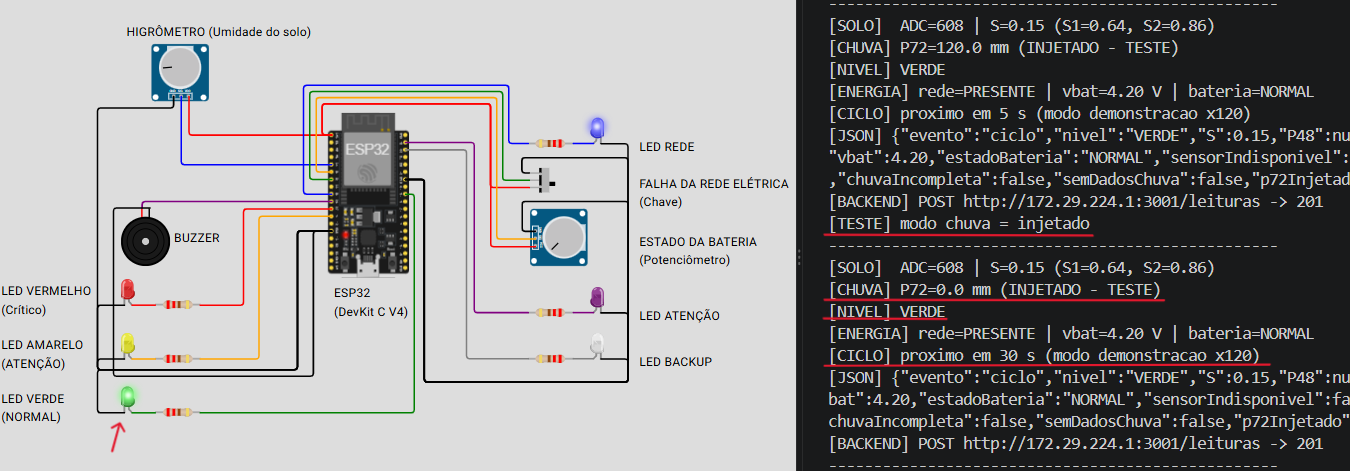
\includegraphics[width=\textwidth]{figures/cap5/C00_intervalo_60min.png}}
\caption{Caso C00: intervalo de 30\,s (60~min em operação) sem chuva e no nível VERDE}
\label{fig:res-c00}
\fonte{Autora, 2026.}
\end{figure}

\paragraph*{Caso C01 --- $S$ baixo e $P_{72}$ baixo}

Entrada: $S = 0{,}11$ e $P_{72} = 10{,}9$\,mm, obtido das APIs
($P_{48} = 4{,}0$\,mm e $P_{24} = 6{,}9$\,mm). Saída esperada: VERDE.
Saída observada: VERDE, com o LED verde aceso
(\autoref{fig:res-c01}).

No painel, com $S = 0{,}11$ e $P_{72} = 30$\,mm informado, o nível foi
VERDE, com a rede presente e a bateria normal (\autoref{fig:res-w05}).

\begin{figure}[H]
\centering
\fbox{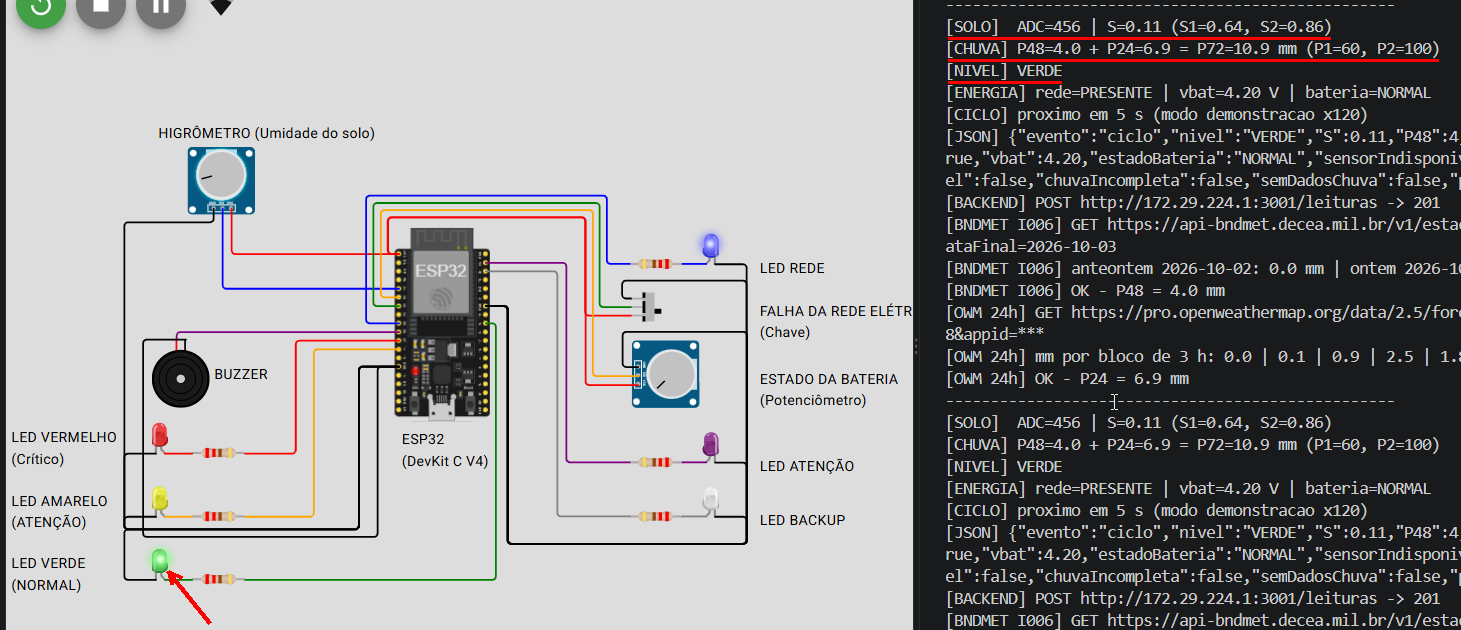
\includegraphics[width=\textwidth]{figures/cap5/C01_Sbaixo_P30.png}}
\caption{Caso C01 na simulação: nível VERDE com $S = 0{,}11$ e $P_{72} = 10{,}9$\,mm}
\label{fig:res-c01}
\fonte{Autora, 2026.}
\end{figure}

\begin{figure}[H]
\centering
\fbox{\includegraphics[width=\textwidth,trim=232 1254 236 0,clip]{figures/cap5/W05_painel_C01_verde.pdf}}
\caption{Painel no cenário do caso C01: VERDE, com $S = 0{,}11$ e $P_{72} = 30$\,mm informado para teste}
\label{fig:res-w05}
\fonte{Autora, 2026.}
\end{figure}

\paragraph*{Caso C02 --- $S$ baixo e $P_{72}$ moderado}

Entrada: $S = 0{,}06$ e $P_{72} = 80$\,mm. Saída esperada: VERDE.
Saída observada: VERDE, com o LED verde aceso (\autoref{fig:res-c02}).

\begin{figure}[H]
\centering
\fbox{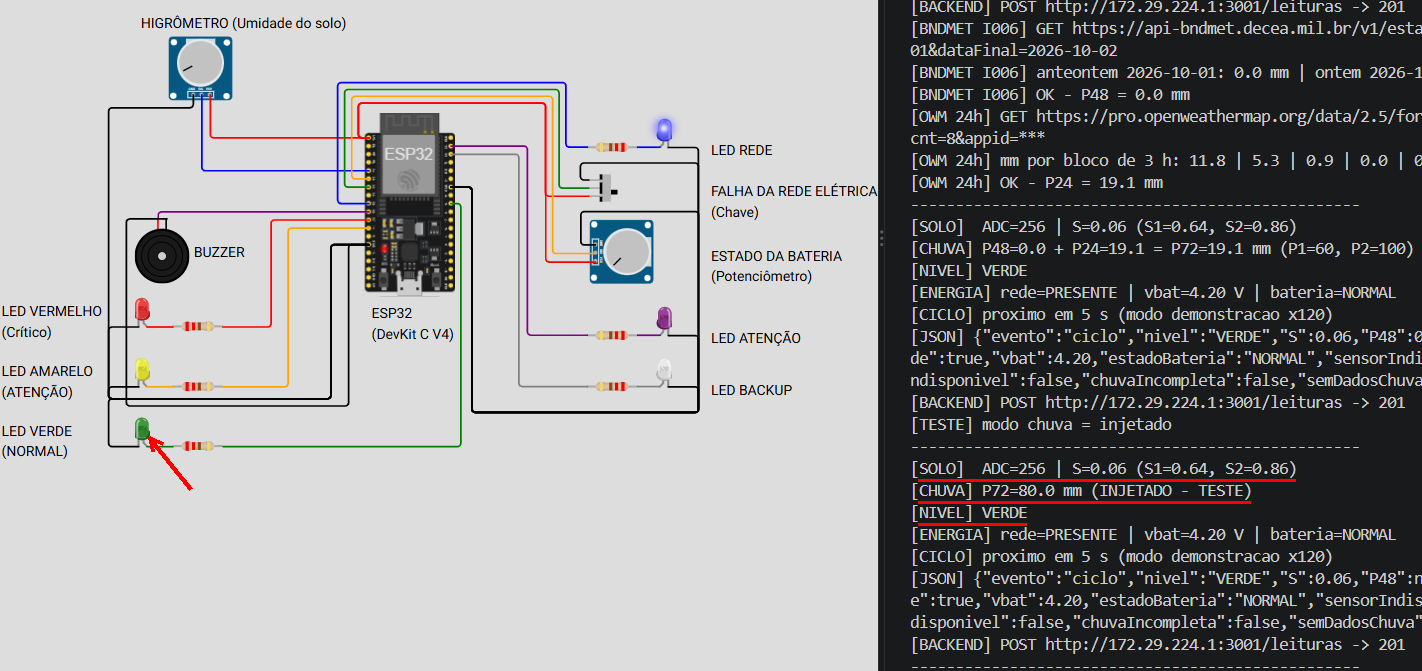
\includegraphics[width=\textwidth]{figures/cap5/C02_Sbaixo_P80.png}}
\caption{Caso C02 na simulação: nível VERDE com $S = 0{,}06$ e $P_{72} = 80$\,mm}
\label{fig:res-c02}
\fonte{Autora, 2026.}
\end{figure}

\paragraph*{Caso C03 --- $S$ baixo e $P_{72}$ alto}

Entrada: $S = 0{,}18$ e $P_{72} = 120$\,mm. Saída esperada: VERDE.
Saída observada: VERDE, com o LED verde aceso (\autoref{fig:res-c03}).
A chuva acima de $P_2$ não elevou o nível, pois $S$ ficou abaixo de
$S_1$.

\begin{figure}[H]
\centering
\fbox{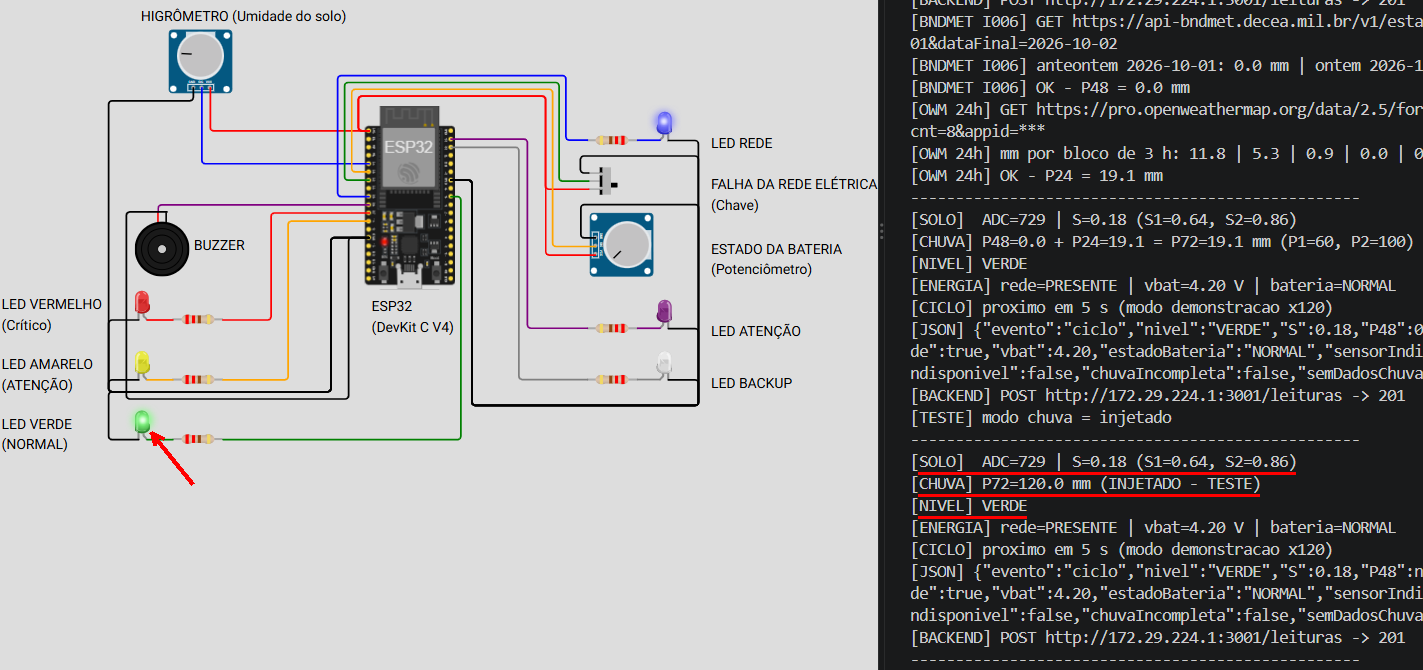
\includegraphics[width=\textwidth]{figures/cap5/C03_Sbaixo_P120.png}}
\caption{Caso C03 na simulação: nível VERDE com $S = 0{,}18$ e $P_{72} = 120$\,mm}
\label{fig:res-c03}
\fonte{Autora, 2026.}
\end{figure}

\paragraph*{Caso C04 --- $S$ moderado e $P_{72}$ baixo}

Entrada: $S = 0{,}80$ e $P_{72} = 19{,}1$\,mm, obtido das APIs. Saída
esperada: VERDE. Saída observada: VERDE, com o LED verde aceso
(\autoref{fig:res-c04}).

\begin{figure}[H]
\centering
\fbox{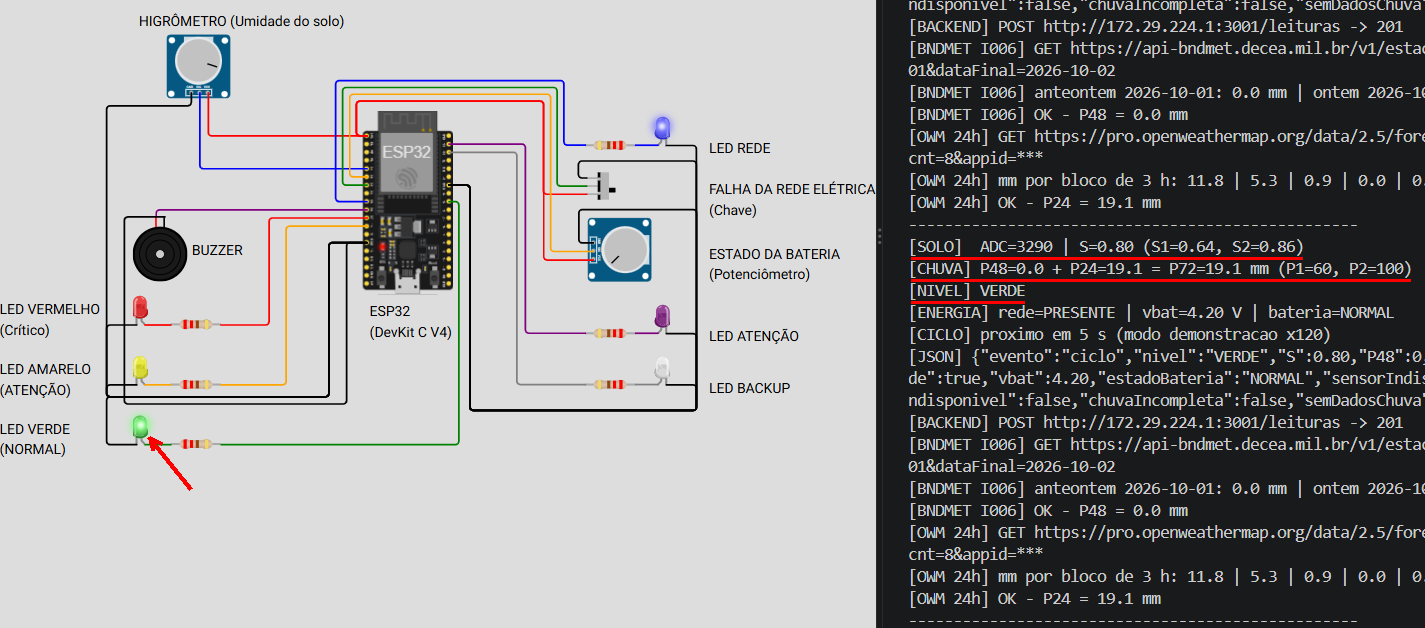
\includegraphics[width=\textwidth]{figures/cap5/C04_Smedio_P30.png}}
\caption{Caso C04 na simulação: nível VERDE com $S = 0{,}80$ e $P_{72} = 19{,}1$\,mm}
\label{fig:res-c04}
\fonte{Autora, 2026.}
\end{figure}

\paragraph*{Caso C05 --- $S$ moderado e $P_{72}$ moderado}

Entrada: $S = 0{,}83$ e $P_{72} = 80$\,mm. Saída esperada: AMARELO.
Saída observada: AMARELO, com o LED amarelo aceso
(\autoref{fig:res-c05}).

No painel, o nível AMARELO apareceu com a orientação do nível e o selo
``Chuva de 72 h injetada para teste''. Os cartões de $P_{48}$ e
$P_{24}$ indicaram que esses valores não foram usados na leitura
(\autoref{fig:res-w06}).

\begin{figure}[H]
\centering
\fbox{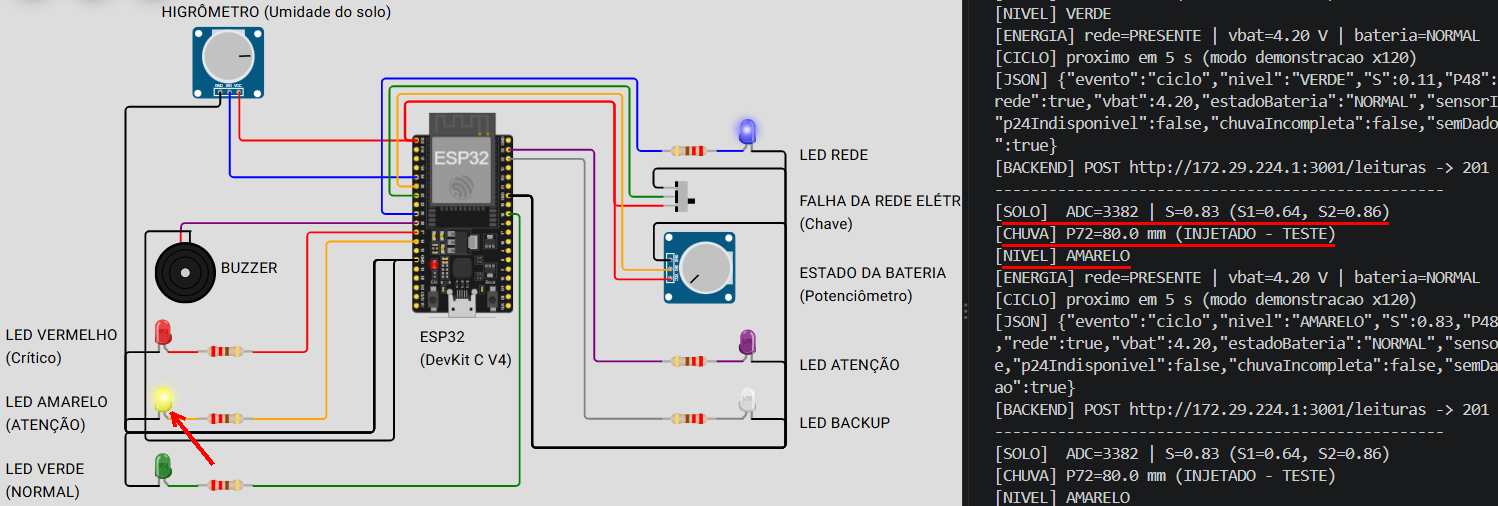
\includegraphics[width=\textwidth]{figures/cap5/C05_Smedio_P80.png}}
\caption{Caso C05 na simulação: nível AMARELO com $S = 0{,}83$ e $P_{72} = 80$\,mm}
\label{fig:res-c05}
\fonte{Autora, 2026.}
\end{figure}

\begin{figure}[H]
\centering
\fbox{\includegraphics[width=\textwidth,trim=232 1254 236 0,clip]{figures/cap5/W06_painel_C05_amarelo.pdf}}
\caption{Painel no cenário do caso C05: AMARELO, com $S = 0{,}83$ e $P_{72} = 80$\,mm informado para teste}
\label{fig:res-w06}
\fonte{Autora, 2026.}
\end{figure}

\paragraph*{Caso C06 --- $S$ moderado e $P_{72}$ alto}

Entrada: $S = 0{,}79$ e $P_{72} = 120$\,mm. Saída esperada: AMARELO.
Saída observada: AMARELO, com o LED amarelo aceso
(\autoref{fig:res-c06}). Mesmo com $P_{72}$ acima de $P_2$, o nível não
chegou a VERMELHO, pois $S$ ficou abaixo de $S_2$.

\begin{figure}[H]
\centering
\fbox{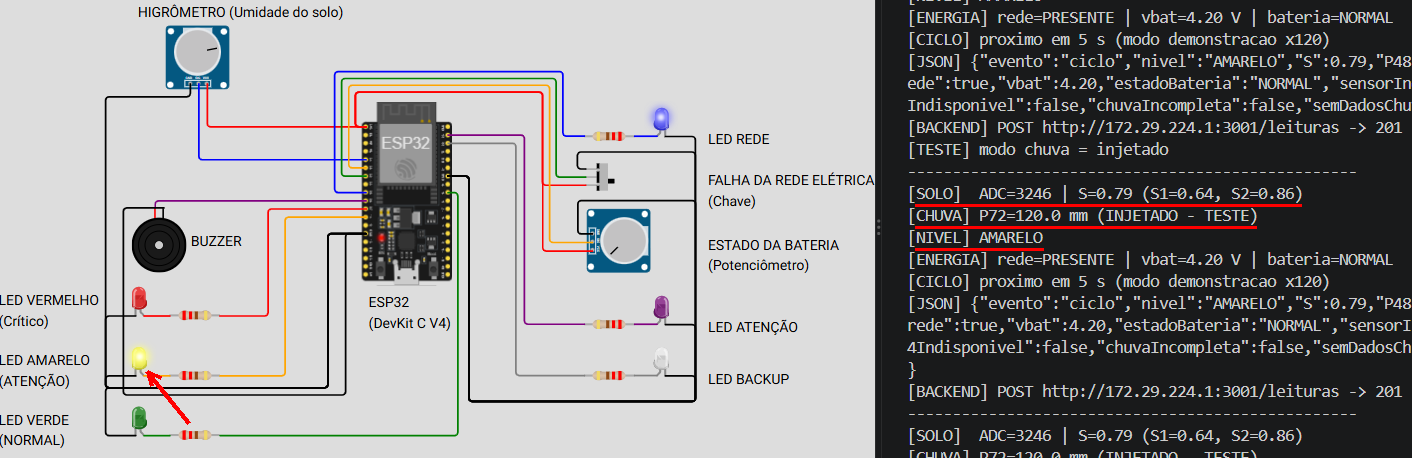
\includegraphics[width=\textwidth]{figures/cap5/C06_Smedio_P120.png}}
\caption{Caso C06 na simulação: nível AMARELO com $S = 0{,}79$ e $P_{72} = 120$\,mm}
\label{fig:res-c06}
\fonte{Autora, 2026.}
\end{figure}

\paragraph*{Caso C07 --- $S$ alto e $P_{72}$ baixo}

Entrada: $S = 0{,}93$ e $P_{72} = 19{,}1$\,mm, obtido das APIs. Saída
esperada: VERDE. Saída observada: VERDE, com o LED verde aceso
(\autoref{fig:res-c07}). O ciclo anterior do mesmo registro, com
$P_{72} = 120$\,mm informado, resultou em VERMELHO.

\begin{figure}[H]
\centering
\fbox{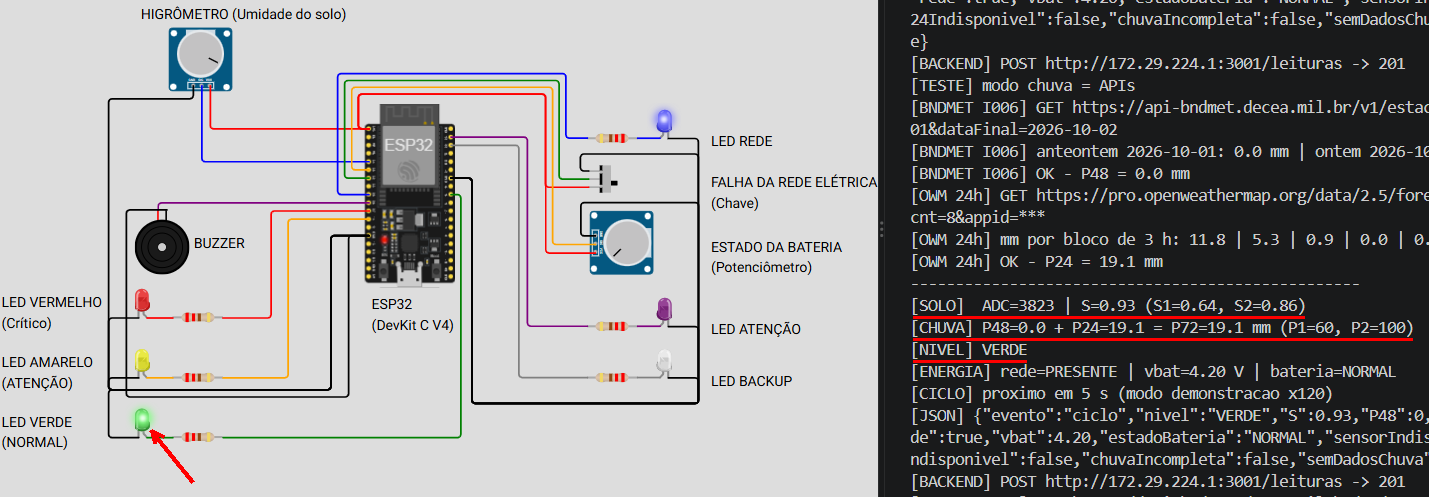
\includegraphics[width=\textwidth]{figures/cap5/C07_Salto_P30.png}}
\caption{Caso C07 na simulação: nível VERDE com $S = 0{,}93$ e $P_{72} = 19{,}1$\,mm}
\label{fig:res-c07}
\fonte{Autora, 2026.}
\end{figure}

\paragraph*{Caso C08 --- $S$ alto e $P_{72}$ moderado}

Entrada: $S = 0{,}93$ e $P_{72} = 80$\,mm. Saída esperada: AMARELO.
Saída observada: AMARELO, com o LED amarelo aceso
(\autoref{fig:res-c08}).

\begin{figure}[H]
\centering
\fbox{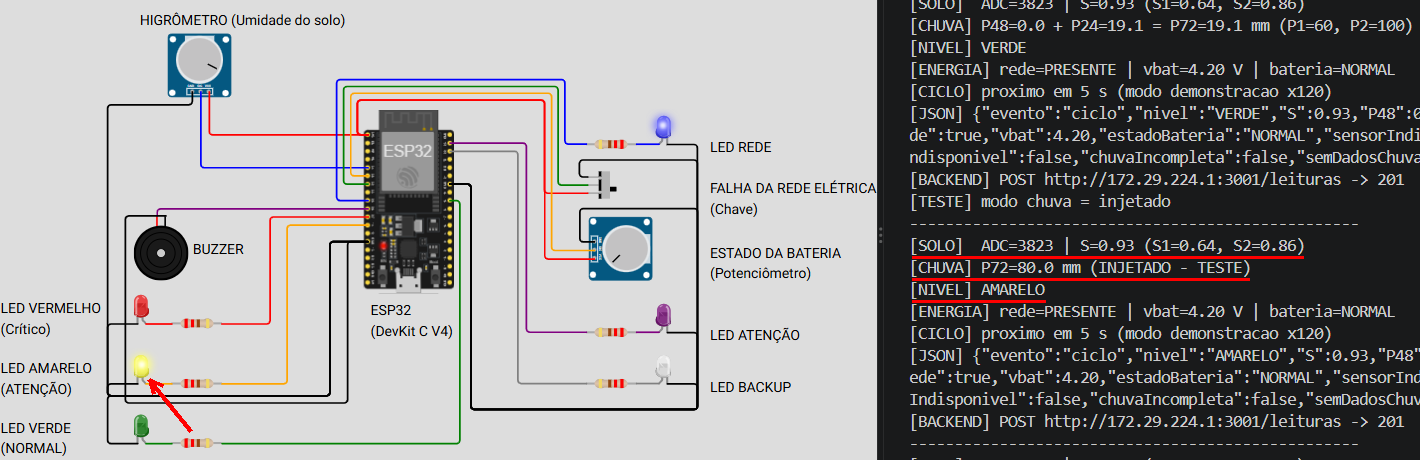
\includegraphics[width=\textwidth]{figures/cap5/C08_Salto_P80.png}}
\caption{Caso C08 na simulação: nível AMARELO com $S = 0{,}93$ e $P_{72} = 80$\,mm}
\label{fig:res-c08}
\fonte{Autora, 2026.}
\end{figure}

\paragraph*{Caso C09 --- $S$ alto e $P_{72}$ alto}

Entrada: $S = 0{,}95$ e $P_{72} = 120$\,mm. Saída esperada: VERMELHO,
com o \textit{buzzer} acionado. Saída observada: VERMELHO, com o LED
vermelho aceso (\autoref{fig:res-c09}).

O sinal de 2300\,Hz do \textit{buzzer} virtual é sonoro e não aparece na
imagem; a evidência registrada é o LED vermelho e a linha
\texttt{[NIVEL] VERMELHO}. No painel, o nível VERMELHO apareceu com a
orientação de deslocamento (\autoref{fig:res-w07}).

\begin{figure}[H]
\centering
\fbox{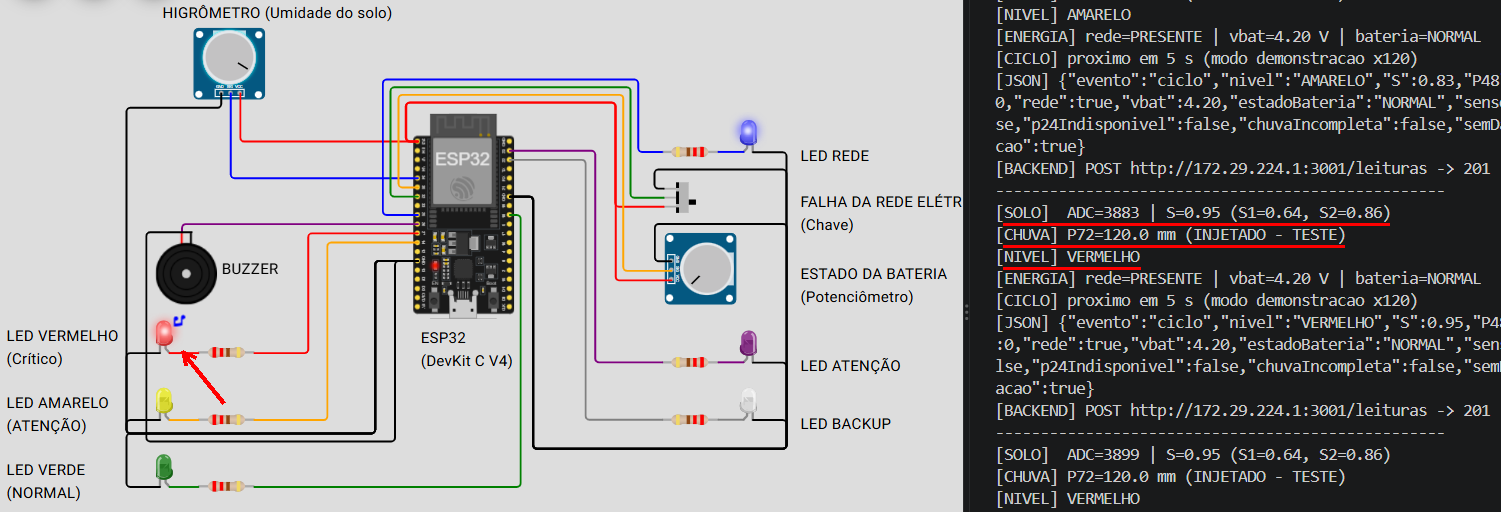
\includegraphics[width=\textwidth]{figures/cap5/C09_Salto_P120.png}}
\caption{Caso C09 na simulação: nível VERMELHO com $S = 0{,}95$ e $P_{72} = 120$\,mm}
\label{fig:res-c09}
\fonte{Autora, 2026.}
\end{figure}

\begin{figure}[H]
\centering
\fbox{\includegraphics[width=\textwidth,trim=232 1254 236 0,clip]{figures/cap5/W07_painel_C09_vermelho.pdf}}
\caption{Painel no cenário do caso C09: VERMELHO, com $S = 0{,}95$ e $P_{72} = 120$\,mm informado para teste}
\label{fig:res-w07}
\fonte{Autora, 2026.}
\end{figure}

% -------------------------------------------------------------
\subsection{Casos de Contingência}
\label{subsec:res-contingencia}
% -------------------------------------------------------------

Os casos X01 a X09 seguem a \autoref{tab:casos-contingencia}. A
\autoref{tab:res-contingencia} resume as entradas e as saídas. Em todos
os casos, o nível observado foi igual ao esperado pela
\autoref{tab:contingencia}.

\begin{table}[htb]
\centering
\caption{Resultados dos casos de contingência na simulação}
\label{tab:res-contingencia}
\small
\begin{tabular}{p{0.9cm}p{5.2cm}p{3.6cm}p{4.4cm}}
\hline
\textbf{Caso} & \textbf{Entrada observada} & \textbf{Saída esperada} & \textbf{Saída observada} \\
\hline
X01 & Higrômetro indisponível (leitura 4095 e 0); $P_{72} = 80$\,mm & AMARELO & AMARELO; aviso de higrômetro indisponível \\
X02 & Higrômetro indisponível; $P_{72} = 120$\,mm & VERMELHO & VERMELHO; LED vermelho \\
X03 & $S = 0{,}96$; sem dados de chuva & AMARELO (caso especial) & AMARELO; ``sem dados de chuva'' \\
X04 & $S = 0{,}72$; sem dados de chuva & VERDE & VERDE; ``sem dados de chuva'' \\
X05 & $S = 0{,}72$; APIs reais, $P_{72} = 10{,}9$\,mm & VERDE & VERDE; dados completos \\
X06 & Higrômetro indisponível; sem dados de chuva & AMARELO (precaução) & AMARELO; os dois avisos \\
X07 & $S = 0{,}96$; dados incompletos, mínimo de 120\,mm & VERMELHO & VERMELHO; ``dados de chuva incompletos'' \\
X08 & $S = 0{,}76$; dados incompletos, mínimo de 80\,mm & AMARELO & AMARELO; ``dados de chuva incompletos'' \\
X09 & $S = 0{,}76$ e $S = 0{,}96$; dados incompletos, mínimo de 30\,mm & VERDE e AMARELO (caso especial) & VERDE e AMARELO; mínimo tratado como falta de dados de chuva \\
\hline
\end{tabular}
\fonte{Autora, 2026, com base nos registros da simulação (valores da simulação).}
\end{table}

\paragraph*{Caso X01 --- higrômetro indisponível e $P_{72}$ moderado}

Entrada: potenciômetro do solo nos extremos do curso (leituras 4095 e
0) e $P_{72} = 80$\,mm. Saída esperada: AMARELO, definido só pela
chuva. Saída observada: ``\texttt{HIGROMETRO INDISPONIVEL}'' nas duas
leituras, nível AMARELO e JSON com \texttt{"S":null} e
\texttt{"sensorIndisponivel":true} (\autoref{fig:res-x01}).

O painel exibiu o nível AMARELO e os avisos ``Sensor de umidade
(higrômetro) indisponível'' e ``O nível foi definido só com a chuva de
72 h'' (\autoref{fig:res-w08}).

\begin{figure}[H]
\centering
\fbox{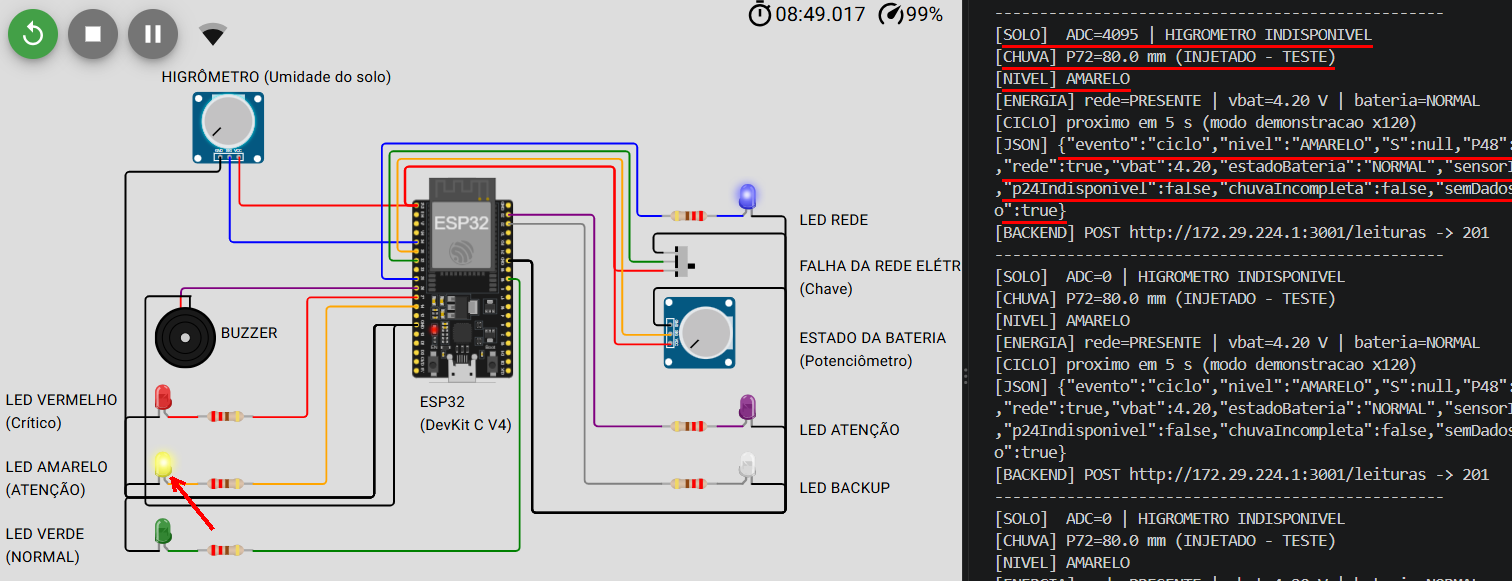
\includegraphics[width=\textwidth]{figures/cap5/X01_sem_sensor_P80.png}}
\caption{Caso X01 na simulação: higrômetro indisponível e nível AMARELO pela chuva ($P_{72} = 80$\,mm)}
\label{fig:res-x01}
\fonte{Autora, 2026.}
\end{figure}

\begin{figure}[H]
\centering
\fbox{\includegraphics[width=\textwidth,trim=232 1292 236 0,clip]{figures/cap5/W08_painel_X01_sem_sensor.pdf}}
\caption{Painel no caso X01: higrômetro indisponível e nível AMARELO definido só pela chuva ($P_{72} = 80$\,mm informado para teste)}
\label{fig:res-w08}
\fonte{Autora, 2026.}
\end{figure}

\paragraph*{Caso X02 --- higrômetro indisponível e $P_{72}$ alto}

Entrada: higrômetro indisponível e $P_{72} = 120$\,mm. Saída esperada:
VERMELHO, definido só pela chuva. Saída observada: VERMELHO, com o LED
vermelho aceso (\autoref{fig:res-x02}).

\begin{figure}[H]
\centering
\fbox{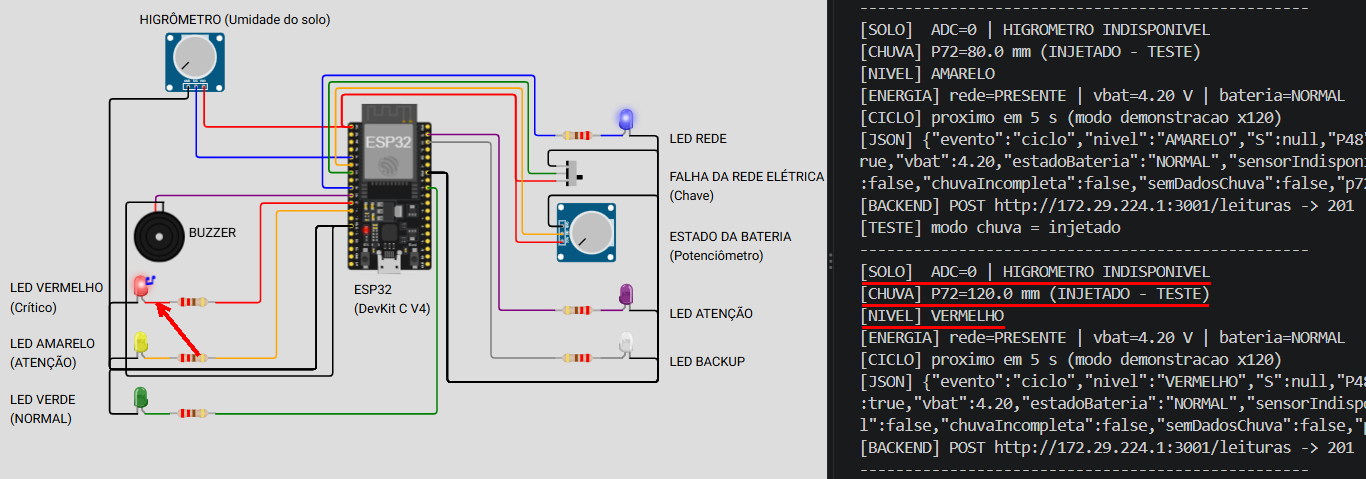
\includegraphics[width=\textwidth]{figures/cap5/X02_sem_sensor_P120.png}}
\caption{Caso X02 na simulação: higrômetro indisponível e nível VERMELHO pela chuva ($P_{72} = 120$\,mm)}
\label{fig:res-x02}
\fonte{Autora, 2026.}
\end{figure}

\paragraph*{Caso X03 --- $S$ alto sem dados de chuva}

Entrada: $S = 0{,}96$ e APIs indisponíveis (\texttt{chuva na}). Saída
esperada: AMARELO, pelo caso especial da \autoref{subsec:contingencia}.
Saída observada: ``\texttt{SEM DADOS DE CHUVA}'', nível AMARELO e JSON
com \texttt{"P72":null} e \texttt{"semDadosChuva":true}
(\autoref{fig:res-x03}).

O painel exibiu o nível AMARELO, os avisos de chuva observada e prevista
indisponíveis e o cartão de $P_{72}$ com ``Sem dados de chuva''
(\autoref{fig:res-w09}).

\begin{figure}[H]
\centering
\fbox{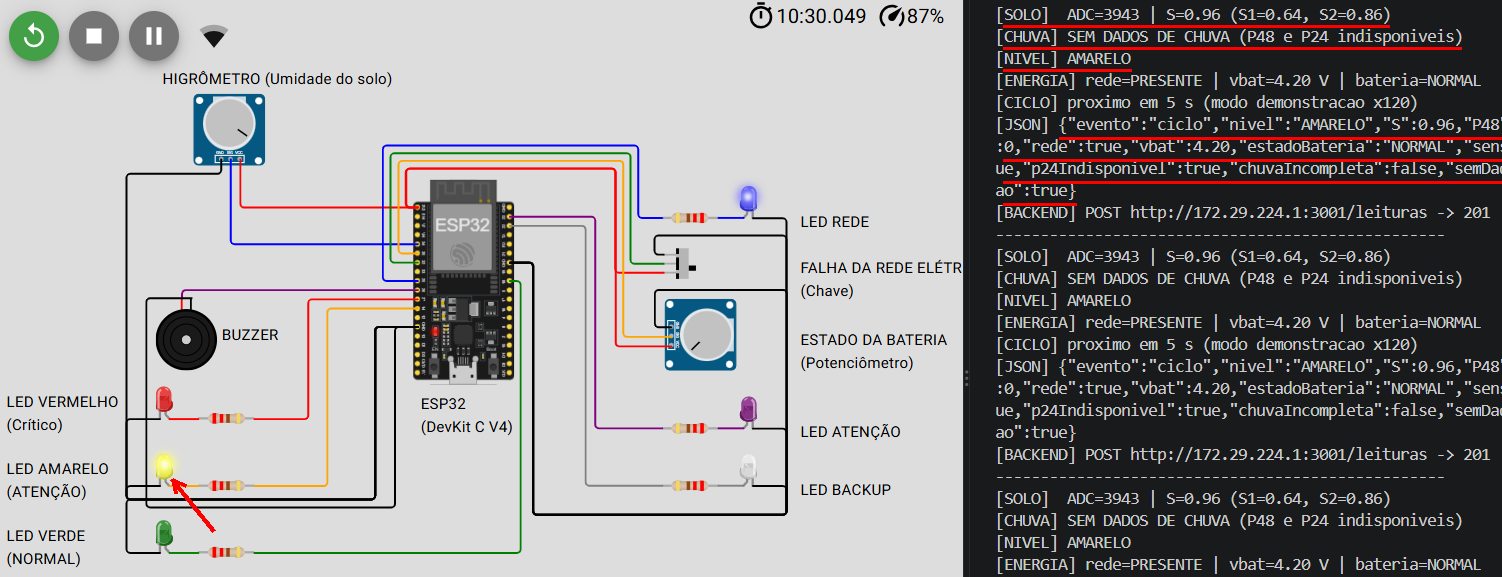
\includegraphics[width=\textwidth]{figures/cap5/X03_sem_chuva_Salto.png}}
\caption{Caso X03 na simulação: sem dados de chuva e $S = 0{,}96$, nível AMARELO (caso especial)}
\label{fig:res-x03}
\fonte{Autora, 2026.}
\end{figure}

\begin{figure}[H]
\centering
\fbox{\includegraphics[width=\textwidth,trim=232 1298 236 0,clip]{figures/cap5/W09_painel_X03_sem_chuva_Salto.pdf}}
\caption{Painel no caso X03: AMARELO com $S = 0{,}96$ e sem dados de chuva (caso especial)}
\label{fig:res-w09}
\fonte{Autora, 2026.}
\end{figure}

\paragraph*{Caso X04 --- $S$ moderado sem dados de chuva}

Entrada: $S = 0{,}72$ e APIs indisponíveis. Saída esperada: VERDE, com
aviso de falta de dados de chuva. Saída observada: VERDE e
``\texttt{SEM DADOS DE CHUVA}'', com próximo ciclo em 30\,s
(\autoref{fig:res-x04}). O painel exibiu o nível VERDE e os mesmos
avisos do caso X03 (\autoref{fig:res-w10}).

\begin{figure}[H]
\centering
\fbox{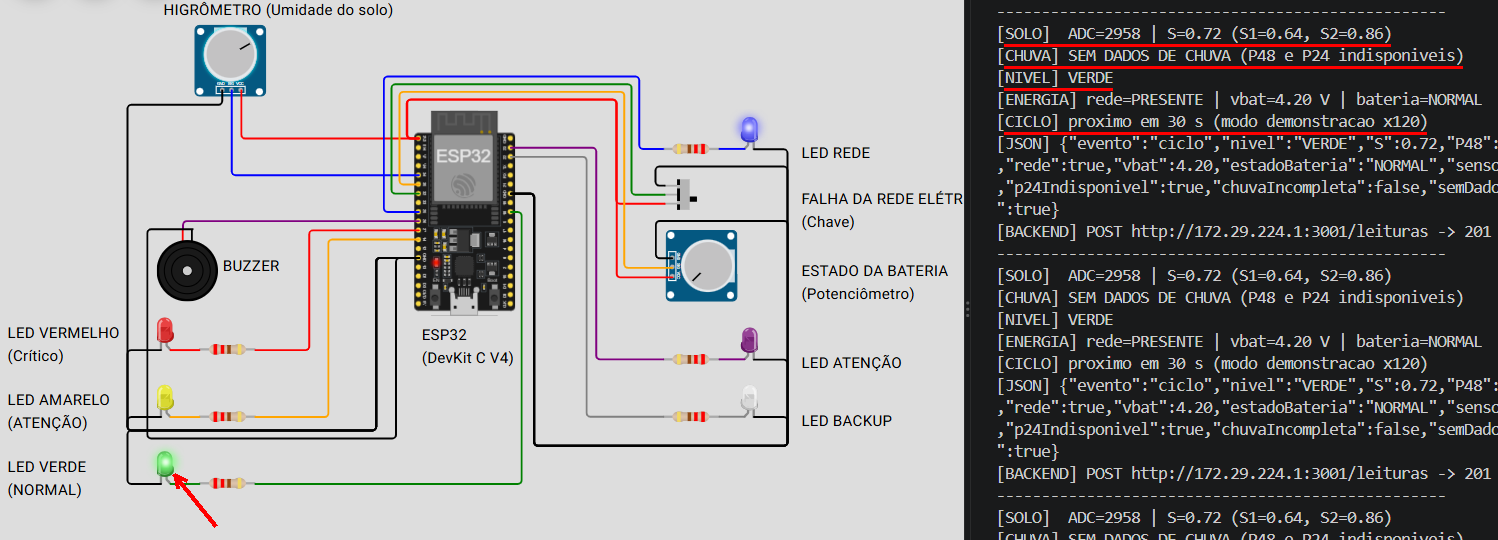
\includegraphics[width=\textwidth]{figures/cap5/X04_sem_chuva_Smedio.png}}
\caption{Caso X04 na simulação: sem dados de chuva e $S = 0{,}72$, nível VERDE}
\label{fig:res-x04}
\fonte{Autora, 2026.}
\end{figure}

\begin{figure}[H]
\centering
\fbox{\includegraphics[width=\textwidth,trim=232 1298 236 0,clip]{figures/cap5/W10_painel_X04_sem_chuva_Smedio.pdf}}
\caption{Painel no caso X04: sem dados de chuva e com $S = 0{,}72$, nível VERDE}
\label{fig:res-w10}
\fonte{Autora, 2026.}
\end{figure}

\paragraph*{Caso X05 --- APIs reais}

Entrada: $S = 0{,}72$ e consulta às APIs em 4 de outubro de 2026. A
BNDMET retornou 0,0\,mm para 2 de outubro e 4,0\,mm para 3 de outubro,
e a soma dos oito blocos da OpenWeatherMap foi de 6,9\,mm. Saída
esperada: $P_{72}$ do dia e nível pela \autoref{tab:matriz}.

Saída observada: ``\texttt{P48=4.0 + P24=6.9 = P72=10.9 mm}'' e nível
VERDE, com o LED verde aceso (\autoref{fig:res-x05}). O painel mostrou
os mesmos valores: $P_{48} = 4{,}0$\,mm, $P_{24} = 6{,}9$\,mm,
$P_{72} = 10{,}9$\,mm e nível VERDE (\autoref{fig:res-w24}).

\begin{figure}[H]
\centering
\fbox{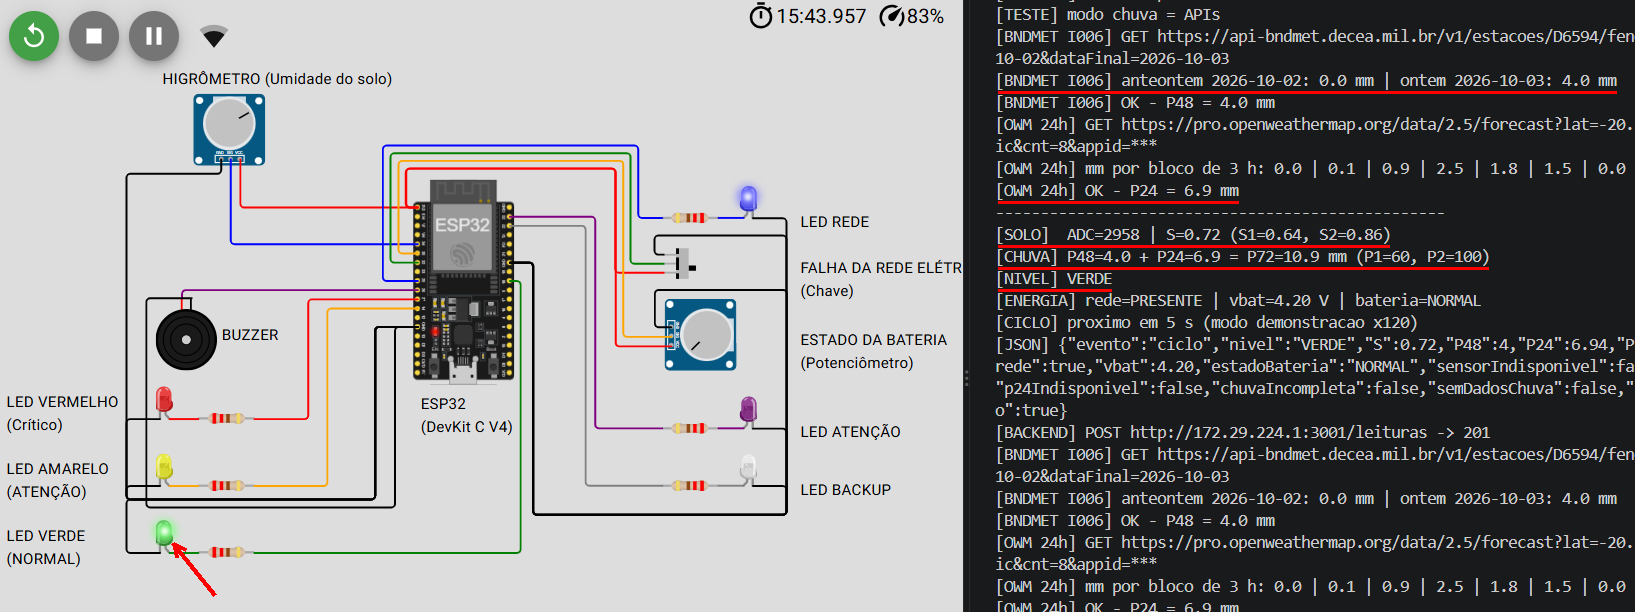
\includegraphics[width=\textwidth]{figures/cap5/X05_apis_reais.png}}
\caption{Caso X05 na simulação: consulta às APIs BNDMET e OpenWeatherMap com dados completos}
\label{fig:res-x05}
\fonte{Autora, 2026.}
\end{figure}

\begin{figure}[H]
\centering
\fbox{\includegraphics[width=\textwidth,trim=232 1290 236 0,clip]{figures/cap5/W24_painel_X05_apis_reais.pdf}}
\caption{Painel no caso X05: leitura com as APIs reais, $P_{72} = 10{,}9$\,mm e nível VERDE}
\label{fig:res-w24}
\fonte{Autora, 2026.}
\end{figure}

\paragraph*{Caso X06 --- higrômetro indisponível e sem dados de chuva}

Entrada: higrômetro indisponível e APIs indisponíveis. Saída esperada:
AMARELO, por precaução. Saída observada:
``\texttt{HIGROMETRO INDISPONIVEL}'', ``\texttt{SEM DADOS DE CHUVA}'' e
nível AMARELO, com \texttt{"sensorIndisponivel":true} e
\texttt{"semDadosChuva":true} no JSON (\autoref{fig:res-x06}).

\begin{figure}[H]
\centering
\fbox{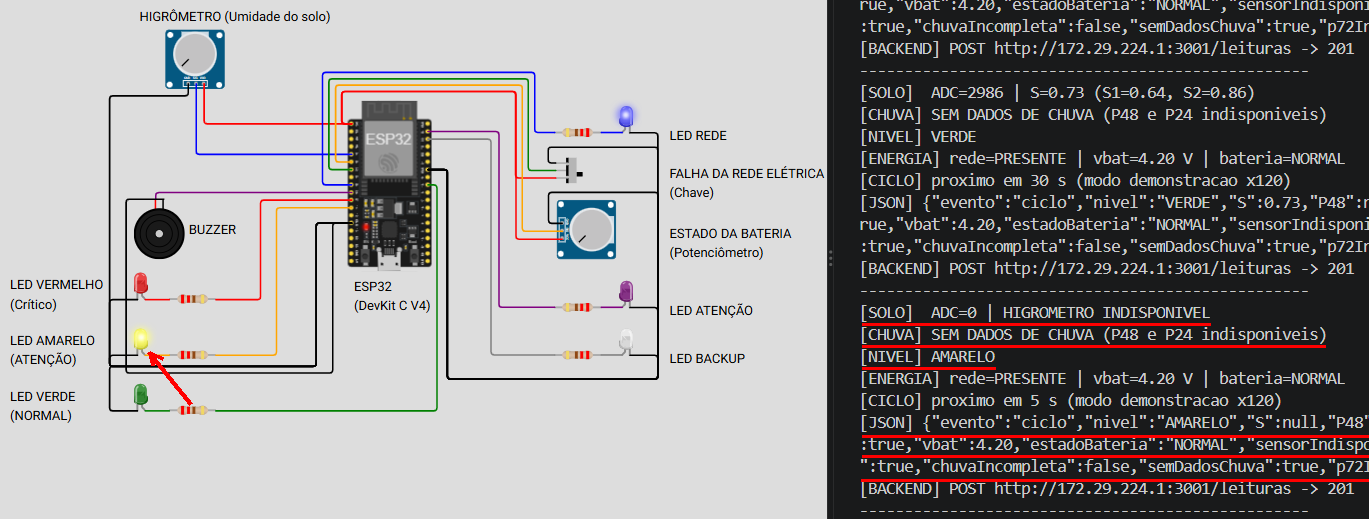
\includegraphics[width=\textwidth]{figures/cap5/X06_sem_sensor_sem_chuva.png}}
\caption{Caso X06 na simulação: higrômetro e dados de chuva indisponíveis, nível AMARELO}
\label{fig:res-x06}
\fonte{Autora, 2026.}
\end{figure}

\paragraph*{Caso X07 --- dados incompletos com mínimo acima de $P_2$}

Entrada: $S = 0{,}96$ e \texttt{chuva parcial 120}, que simula um dia
sem registro na BNDMET. Saída esperada: VERMELHO, avaliado com o mínimo
garantido. Saída observada: ``\texttt{DADOS DE CHUVA INCOMPLETOS -
P72 >= 120.0 mm}'' e nível VERMELHO (\autoref{fig:res-x07}).

O JSON trouxe \texttt{"P72":null}, \texttt{"p72Minimo":120},
\texttt{"p48DiasNulos":1} e \texttt{"chuvaIncompleta":true}.

\begin{figure}[H]
\centering
\fbox{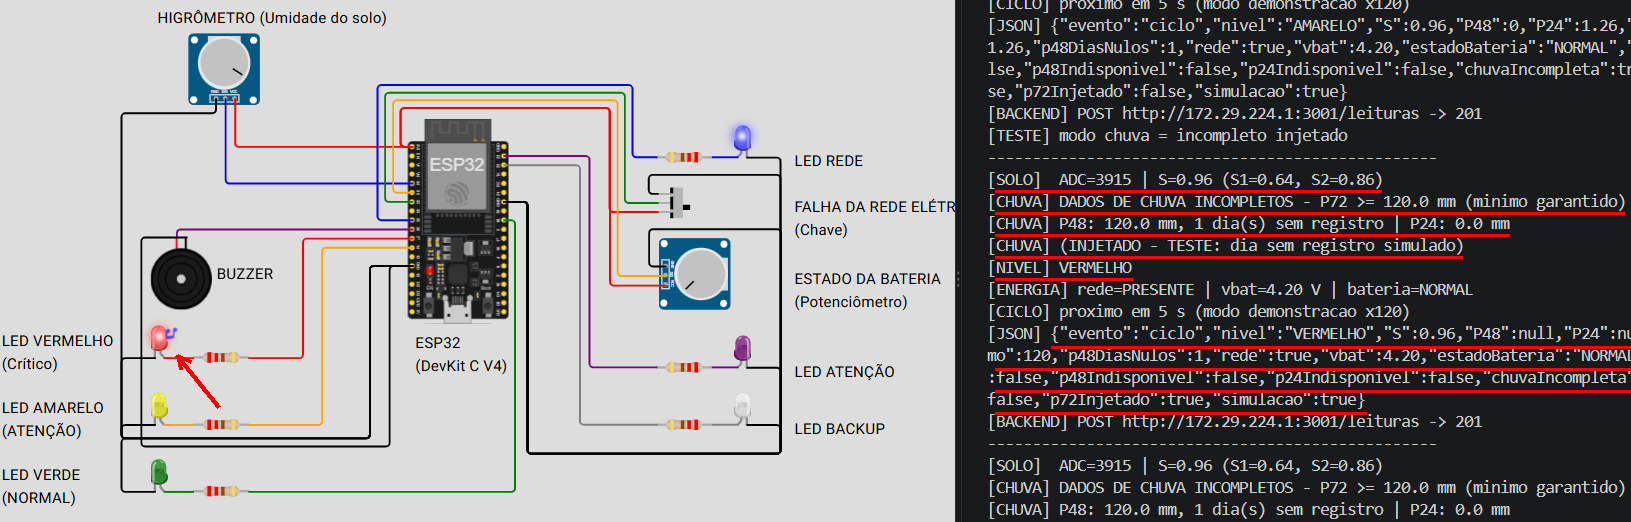
\includegraphics[width=\textwidth]{figures/cap5/X07_incompleto_Salto_P120.png}}
\caption{Caso X07 na simulação: dados de chuva incompletos, mínimo de 120\,mm e nível VERMELHO}
\label{fig:res-x07}
\fonte{Autora, 2026.}
\end{figure}

\paragraph*{Caso X08 --- dados incompletos com mínimo entre $P_1$ e $P_2$}

Entrada: $S = 0{,}76$ e \texttt{chuva parcial 80}. Saída esperada:
AMARELO, avaliado com o mínimo garantido. Saída observada:
``\texttt{DADOS DE CHUVA INCOMPLETOS - P72 >= 80.0 mm}'' e nível
AMARELO, com o LED amarelo aceso e \texttt{"p72Minimo":80} no JSON
(\autoref{fig:res-x08}).

O painel exibiu o nível AMARELO e os avisos ``1 dia(s) sem registro na
estação BNDMET'' e ``Dados de chuva incompletos --- P72 $\geq$ 80,0 mm.
O nível foi definido com esse mínimo'' (\autoref{fig:res-w21}).

\begin{figure}[H]
\centering
\fbox{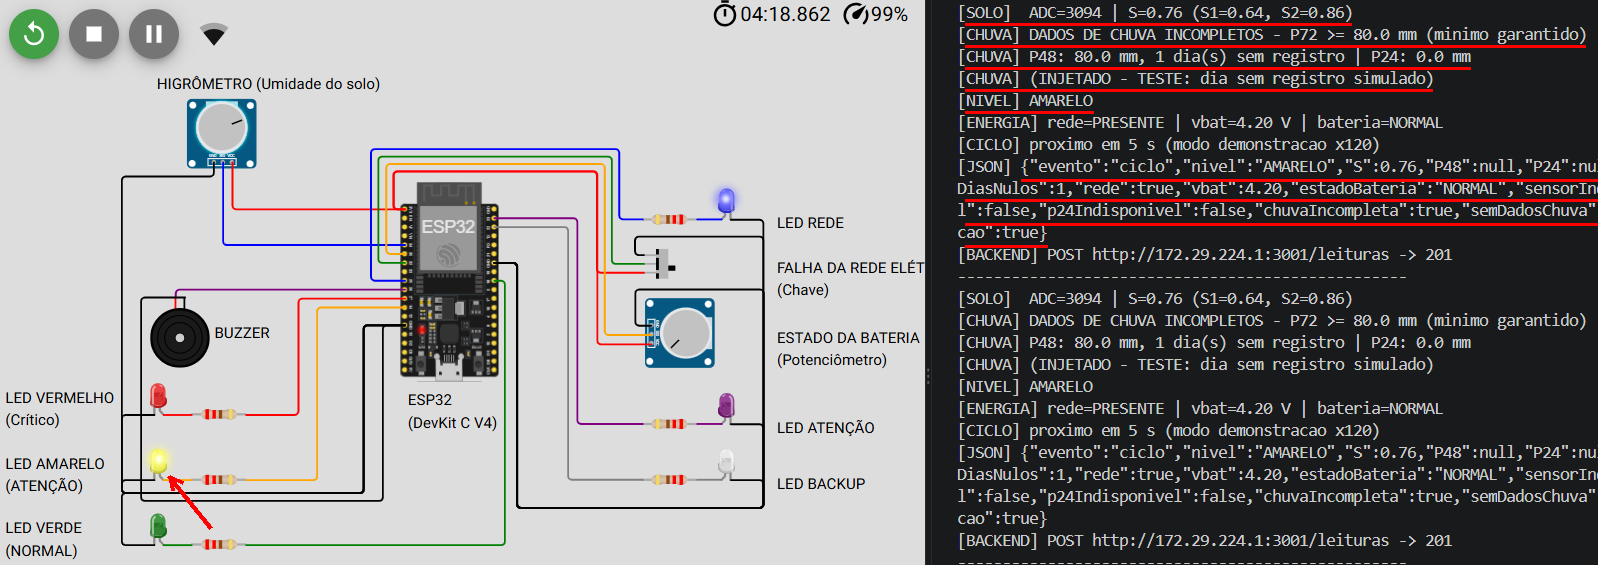
\includegraphics[width=\textwidth]{figures/cap5/X08_incompleto_Smedio_P80.png}}
\caption{Caso X08 na simulação: dados de chuva incompletos, mínimo de 80\,mm e nível AMARELO}
\label{fig:res-x08}
\fonte{Autora, 2026.}
\end{figure}

\begin{figure}[H]
\centering
\fbox{\includegraphics[width=\textwidth,trim=232 1328 236 0,clip]{figures/cap5/W21_painel_incompleta_dia_nulo.pdf}}
\caption{Painel no caso X08: dados de chuva incompletos, mínimo de 80\,mm e nível AMARELO}
\label{fig:res-w21}
\fonte{Autora, 2026.}
\end{figure}

\paragraph*{Caso X09 --- dados incompletos com mínimo abaixo de $P_1$}

Entrada: \texttt{chuva parcial 30}, com $S = 0{,}76$ e, em seguida,
$S = 0{,}96$. Saída esperada: mínimo garantido de 30\,mm, abaixo de
$P_1$, tratado como falta de dados de chuva; VERDE com $S < S_2$ e
AMARELO com $S \geq S_2$ (caso especial).

Saída observada: ``\texttt{DADOS DE CHUVA INCOMPLETOS - P72 >= 30.0
mm}'' e ``\texttt{Minimo abaixo de P1: tratado como sem dados de
chuva}'' nos dois ciclos. O nível foi VERDE com $S = 0{,}76$ e AMARELO
com $S = 0{,}96$, com o LED amarelo aceso (\autoref{fig:res-x09}).

\begin{figure}[H]
\centering
\fbox{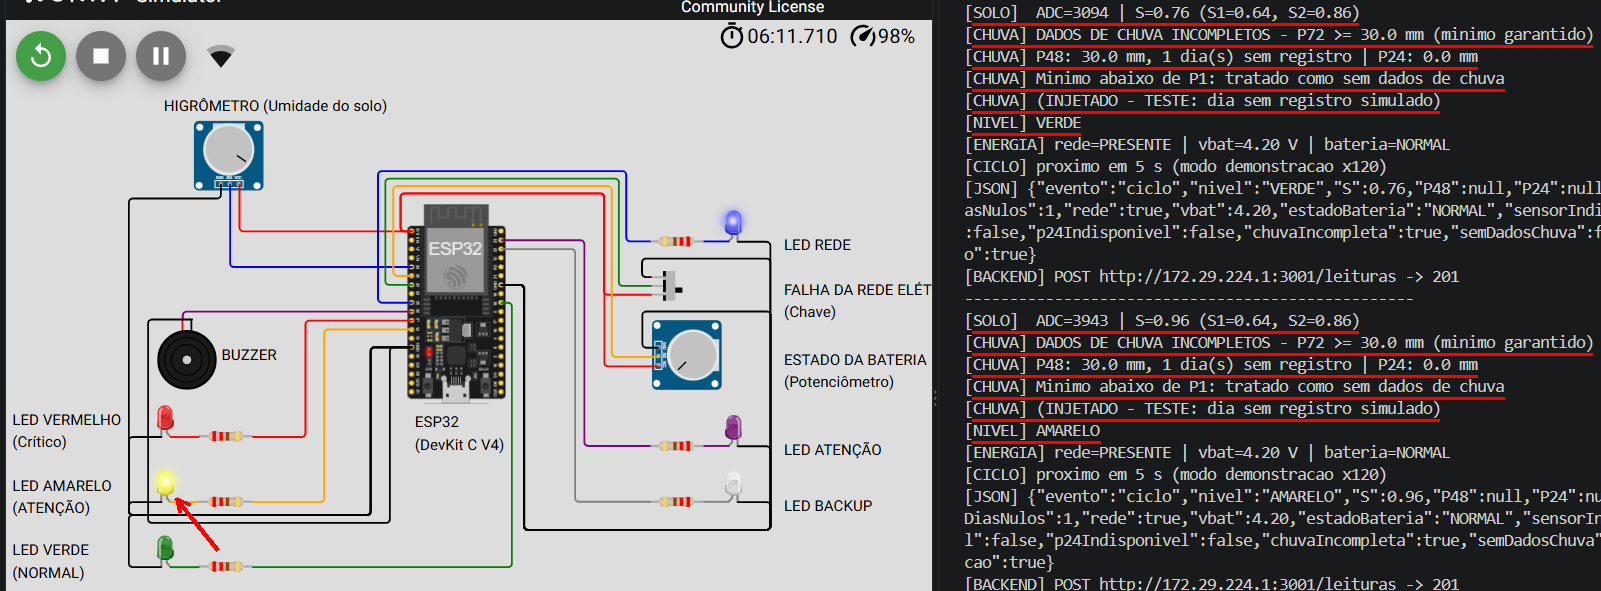
\includegraphics[width=\textwidth]{figures/cap5/X09_incompleto_Salto_P30.png}}
\caption{Caso X09 na simulação: dados de chuva incompletos, mínimo de 30\,mm; VERDE com $S = 0{,}76$ e AMARELO com $S = 0{,}96$ (caso especial)}
\label{fig:res-x09}
\fonte{Autora, 2026.}
\end{figure}

O painel exibiu o nível AMARELO e o aviso de que a chuva não entrou na
regra e o nível foi definido só com a saturação do solo
(\autoref{fig:res-w23}). Com o mínimo abaixo de $P_1$ e $S$ moderado, o
nível é VERDE, como na \autoref{fig:res-w22}, uma leitura enviada por
requisição manual em que a previsão da OpenWeatherMap ficou
indisponível.

\begin{figure}[H]
\centering
\fbox{\includegraphics[width=\textwidth,trim=232 1290 236 0,clip]{figures/cap5/W23_painel_incompleta_Salto.pdf}}
\caption{Painel no caso X09: dados de chuva incompletos, mínimo abaixo de $P_1$ e $S = 0{,}96$, nível AMARELO}
\label{fig:res-w23}
\fonte{Autora, 2026.}
\end{figure}

\begin{figure}[H]
\centering
\fbox{\includegraphics[width=\textwidth,trim=232 2506 236 0,clip]{figures/cap5/W22_painel_incompleta_owm_fora.pdf}}
\caption{Painel com previsão indisponível, mínimo de 30\,mm e $S = 0{,}70$: VERDE (leitura enviada por requisição manual, teste da interface)}
\label{fig:res-w22}
\fonte{Autora, 2026.}
\end{figure}

% =============================================================
\section{Supervisão de Energia}
\label{sec:res-energia}
% =============================================================

Os casos E01 a E04 seguem a \autoref{tab:casos-energia}. A rede
elétrica foi representada pela chave, e a tensão da bateria, pelo
potenciômetro, conforme a \autoref{tab:componentes-wokwi}. O nível de
alerta permaneceu VERDE em todos os casos, para isolar a energia.

A \autoref{tab:res-energia} resume os resultados. As tensões são
valores da simulação, e não medições de uma bateria.

\begin{table}[htb]
\centering
\caption{Resultados dos casos de energia na simulação}
\label{tab:res-energia}
\small
\begin{tabular}{p{1.0cm}p{4.4cm}p{3.8cm}p{4.8cm}}
\hline
\textbf{Caso} & \textbf{Entrada} & \textbf{Saída esperada} & \textbf{Saída observada} \\
\hline
E01 & Rede presente; 4,20\,V & Normal; LED REDE & \texttt{rede=PRESENTE}, \texttt{bateria=NORMAL}; LED REDE aceso \\
E02 & Rede ausente; 4,20\,V & Falta de rede; LED BACKUP & \texttt{rede=AUSENTE (backup)}; evento de energia; LED BACKUP aceso \\
E03a & Rede ausente; 3,15\,V & Bateria baixa; LED ATENÇÃO piscando & \texttt{bateria=BAIXA}; LED ATENÇÃO aceso no instante do registro \\
E03b & Rede ausente; 2,61\,V & Bateria crítica; LED ATENÇÃO piscando & \texttt{bateria=CRITICA}; LED ATENÇÃO aceso no instante do registro \\
E04a & Rede presente; 3,61\,V & Normal, com indicação de recarga & \texttt{NORMAL (recarregando)}; 557\,s de 585\,s \\
E04b & Rede presente; 3,60\,V após 585\,s & Falha, sem indicação de recarga; LED ATENÇÃO aceso & \texttt{bateria=FALHA}, sem ``recarregando''; LED ATENÇÃO aceso \\
E04c & Rede presente; 4,20\,V & Volta ao normal & \texttt{bateria=NORMAL}; evento de energia \\
\hline
\end{tabular}
\fonte{Autora, 2026, com base nos registros da simulação (valores da simulação).}
\end{table}

\paragraph*{Caso E01 --- rede presente}

Entrada: chave ligada e bateria em 4,20\,V. Saída esperada: LED REDE
aceso e bateria normal. Saída observada:
``\texttt{rede=PRESENTE | vbat=4.20 V | bateria=NORMAL}'', com o LED
REDE aceso e os LEDs BACKUP e ATENÇÃO apagados (\autoref{fig:res-e01}).

\begin{figure}[H]
\centering
\fbox{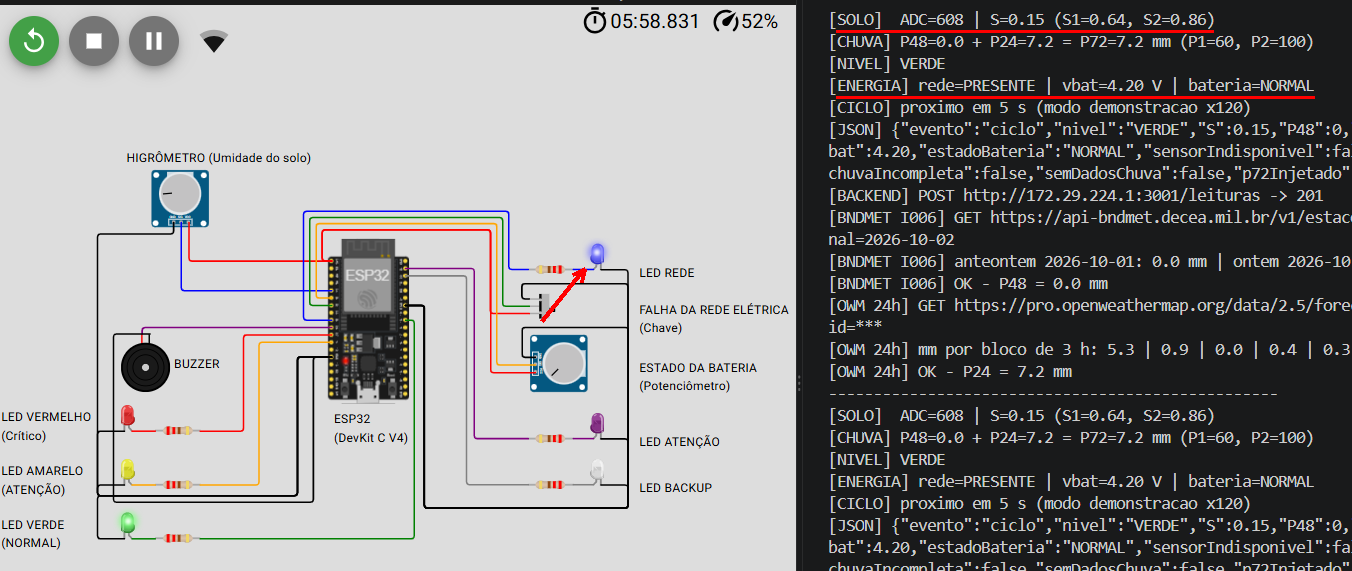
\includegraphics[width=\textwidth]{figures/cap5/E01_rede_ok.png}}
\caption{Caso E01 na simulação: rede presente e bateria normal}
\label{fig:res-e01}
\fonte{Autora, 2026.}
\end{figure}

\paragraph*{Caso E02 --- falta de rede}

Entrada: chave desligada, com a bateria em 4,20\,V, $S = 0{,}29$ e
$P_{72} = 30$\,mm. Saída esperada: LED BACKUP aceso, aviso de falta de
rede e nível de alerta mantido. Saída observada:
``\texttt{rede=AUSENTE (backup)}'', JSON com \texttt{"evento":"energia"}
e \texttt{"rede":false}, e LED BACKUP aceso (\autoref{fig:res-e02}).

Os ciclos seguintes continuaram a calcular o nível (VERDE) e a enviar
as leituras. O painel exibiu ``Ausente: operando na bateria''
(\autoref{fig:res-w11}).

\begin{figure}[H]
\centering
\fbox{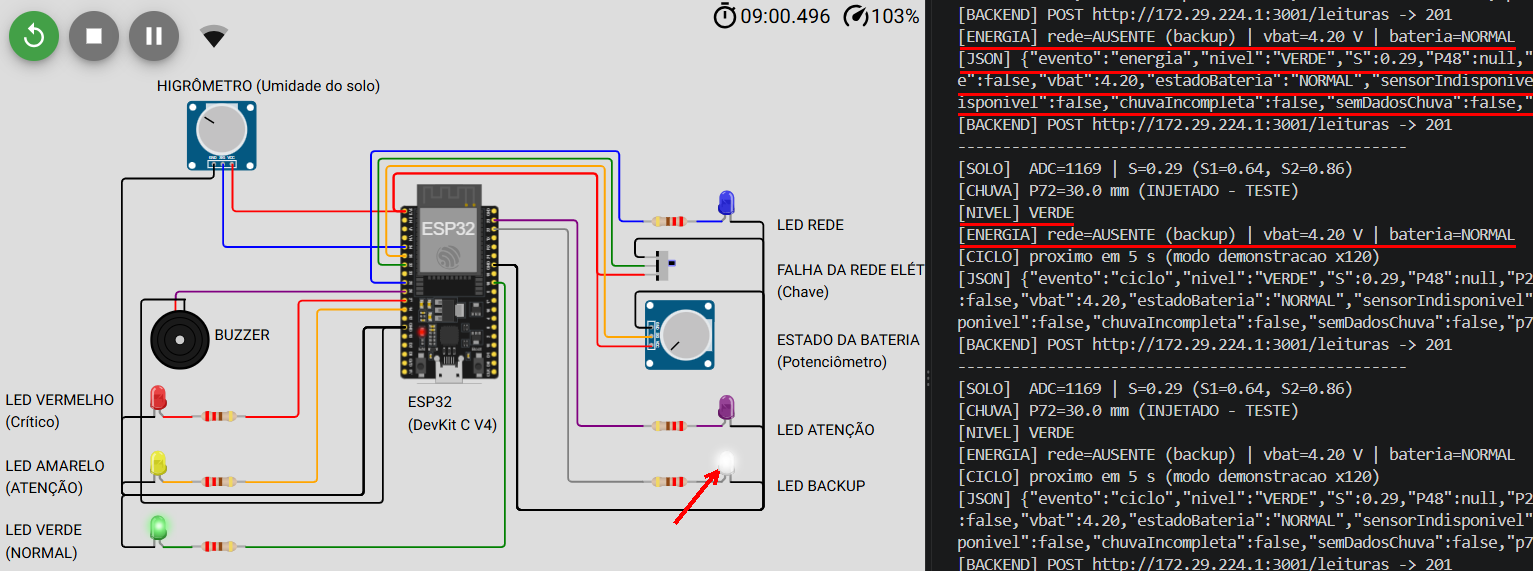
\includegraphics[width=\textwidth]{figures/cap5/E02_falta_rede.png}}
\caption{Caso E02 na simulação: falta de rede, operação na bateria e nível de alerta mantido}
\label{fig:res-e02}
\fonte{Autora, 2026.}
\end{figure}

\begin{figure}[H]
\centering
\fbox{\includegraphics[width=\textwidth,trim=232 1254 236 0,clip]{figures/cap5/W11_painel_E02_falta_rede.pdf}}
\caption{Painel no caso E02: rede elétrica ausente e operação na bateria}
\label{fig:res-w11}
\fonte{Autora, 2026.}
\end{figure}

\paragraph*{Caso E03 --- bateria baixa e bateria crítica}

Entrada: rede ausente e tensão reduzida no potenciômetro. Saída
esperada: bateria baixa abaixo de 3,30\,V e crítica abaixo de 3,00\,V
(\autoref{tab:estados-energia}), com o LED ATENÇÃO piscando.

Saída observada: em 3,15\,V, ``\texttt{bateria=BAIXA}'', com JSON
\texttt{"estadoBateria":"BAIXA"} e LED ATENÇÃO aceso
(\autoref{fig:res-e03a}).

\begin{figure}[H]
\centering
\fbox{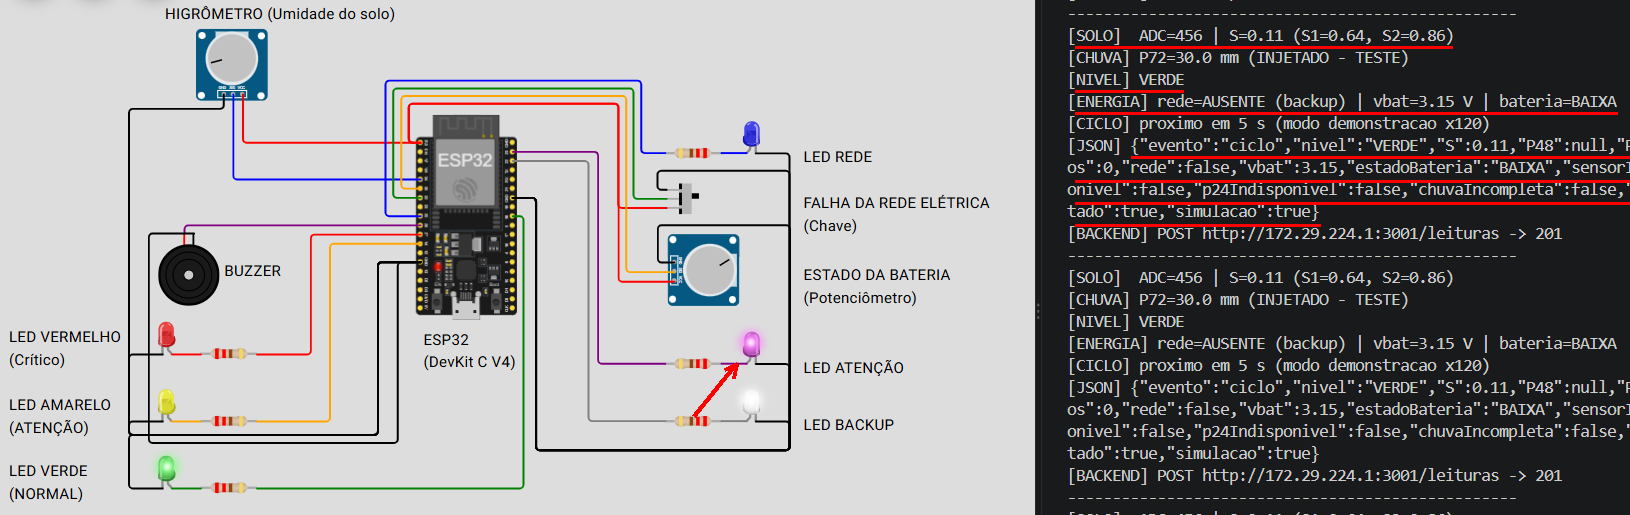
\includegraphics[width=\textwidth]{figures/cap5/E03a_bateria_baixa.png}}
\caption{Caso E03a na simulação: bateria baixa (3,15\,V) com a rede ausente}
\label{fig:res-e03a}
\fonte{Autora, 2026.}
\end{figure}

Em 2,61\,V, a bateria passou a ``\texttt{CRITICA}'', com
\texttt{"estadoBateria":"CRITICA"} no JSON (\autoref{fig:res-e03b}). O
LED ATENÇÃO aparece aceso nos dois registros, que captam um instante do
piscar.

\begin{figure}[H]
\centering
\fbox{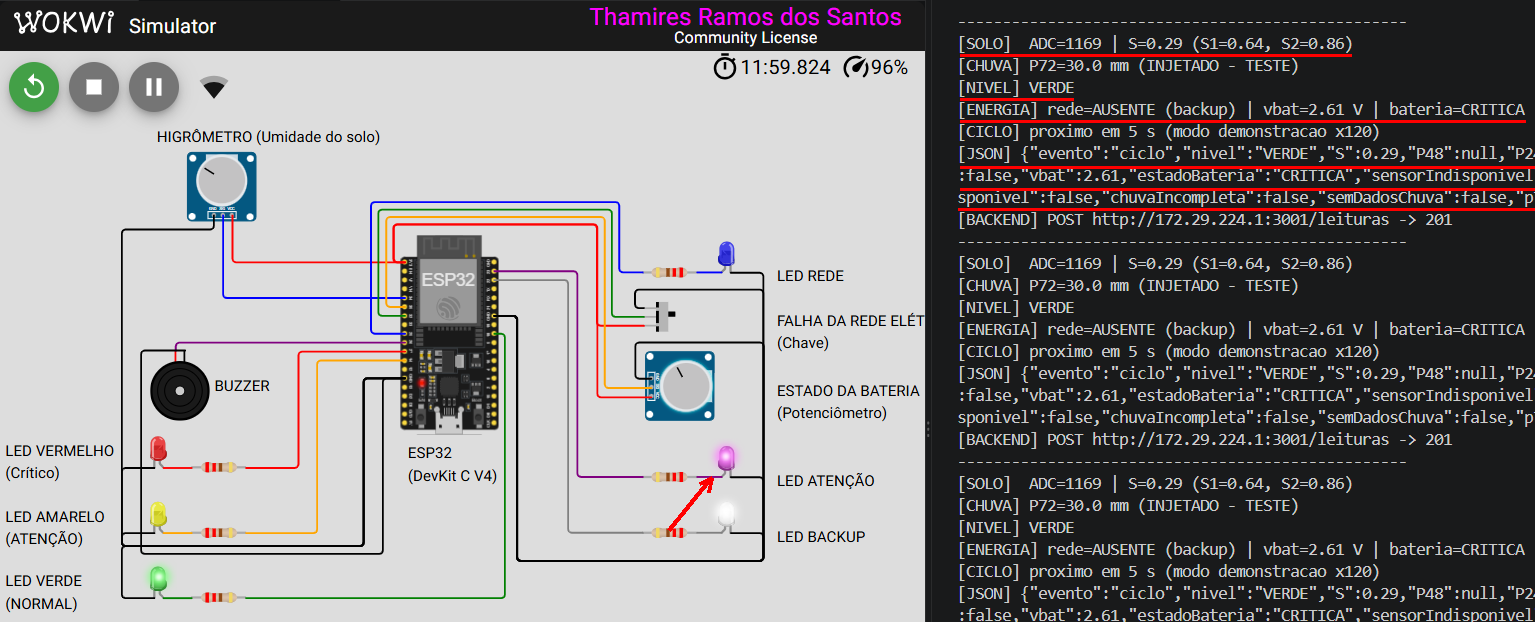
\includegraphics[width=\textwidth]{figures/cap5/E03b_bateria_critica.png}}
\caption{Caso E03b na simulação: bateria crítica (2,61\,V) com a rede ausente}
\label{fig:res-e03b}
\fonte{Autora, 2026.}
\end{figure}

O painel exibiu ``Baixa · 3,15 V'' (\autoref{fig:res-w12}) e
``Crítica · 2,61 V'' (\autoref{fig:res-w12b}).

\begin{figure}[H]
\centering
\fbox{\includegraphics[width=\textwidth,trim=232 1254 236 0,clip]{figures/cap5/W12_painel_E03_bateria_baixa.pdf}}
\caption{Painel no caso E03a: bateria baixa (3,15\,V, valor da simulação)}
\label{fig:res-w12}
\fonte{Autora, 2026.}
\end{figure}

\begin{figure}[H]
\centering
\fbox{\includegraphics[width=\textwidth,trim=232 1254 236 0,clip]{figures/cap5/W12b_painel_E03_bateria_critica.pdf}}
\caption{Painel no caso E03b: bateria crítica (2,61\,V, valor da simulação)}
\label{fig:res-w12b}
\fonte{Autora, 2026.}
\end{figure}

\paragraph*{Caso E04 --- recarga e falha de bateria}

Entrada: rede religada e bateria mantida abaixo de 4,20\,V. Saída
esperada: durante $T_{\mathrm{carga}}$ (585\,s no modo de demonstração),
estado normal com indicação de recarga; após esse tempo, falha de
bateria, sem a indicação de recarga.

Saída observada: em 3,61\,V, ``\texttt{bateria=NORMAL (recarregando)}''
e ``\texttt{recarga: 557 s de 585 s ate FALHA}''
(\autoref{fig:res-e04a}). Após 585\,s, ``\texttt{bateria=FALHA}'', sem
``recarregando'', JSON com \texttt{"estadoBateria":"FALHA"} e LED
ATENÇÃO aceso (\autoref{fig:res-e04b}).

\begin{figure}[H]
\centering
\fbox{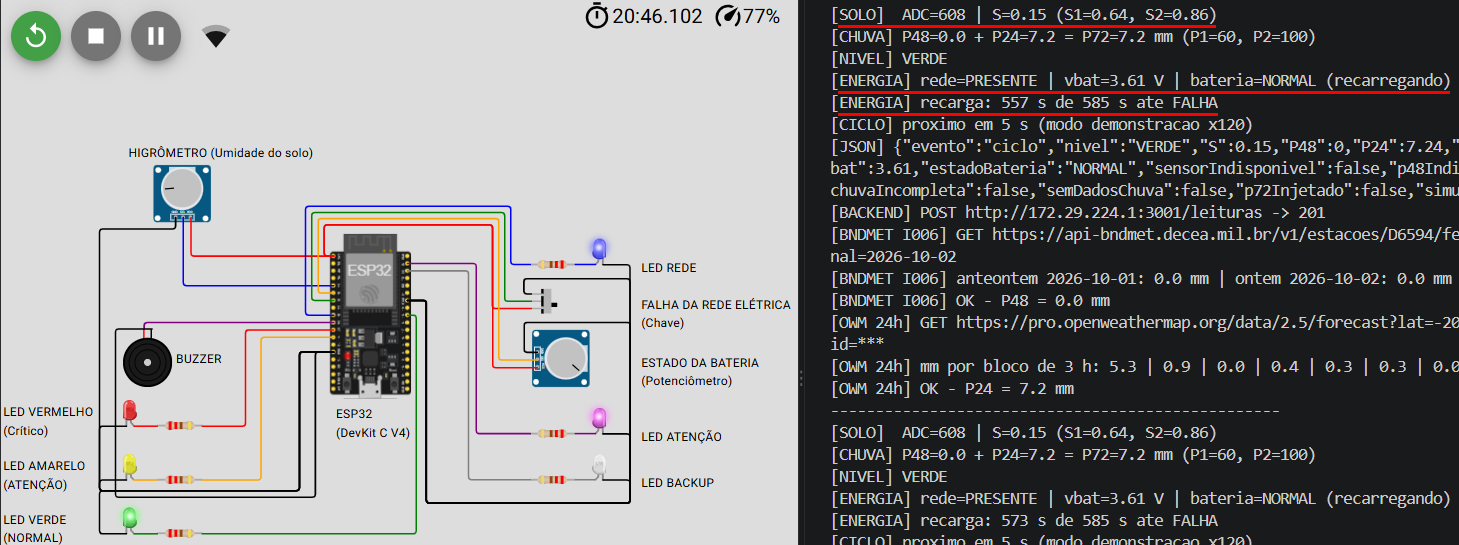
\includegraphics[width=\textwidth]{figures/cap5/E04a_recarga.png}}
\caption{Caso E04a na simulação: rede presente e bateria em recarga (contagem até $T_{\mathrm{carga}}$)}
\label{fig:res-e04a}
\fonte{Autora, 2026.}
\end{figure}

\begin{figure}[H]
\centering
\fbox{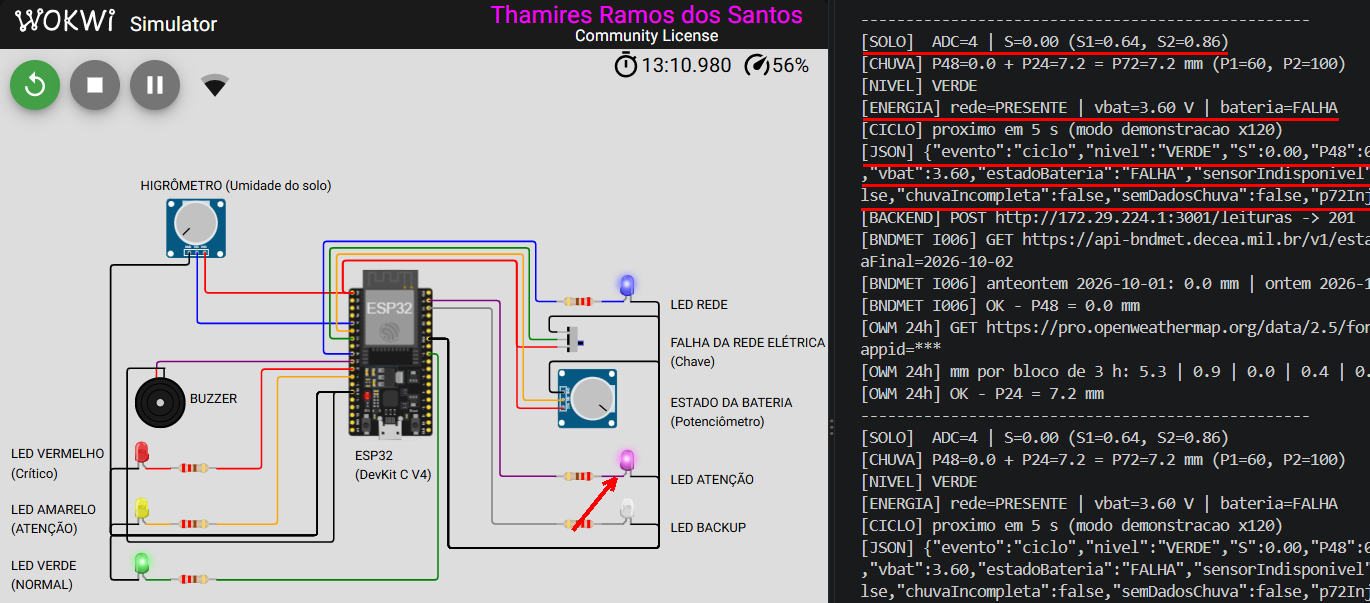
\includegraphics[width=\textwidth]{figures/cap5/E04b_falha_bateria.png}}
\caption{Caso E04b na simulação: falha de bateria após $T_{\mathrm{carga}}$, sem indicação de recarga}
\label{fig:res-e04b}
\fonte{Autora, 2026.}
\end{figure}

Com o potenciômetro levado a 4,20\,V, que representa a troca da
bateria, o estado voltou a normal e um novo evento de energia foi
enviado, com o LED ATENÇÃO apagado (\autoref{fig:res-e04c}). Em outro
registro do mesmo cenário, o painel exibiu ``Falha: substituir''
(\autoref{fig:res-w13}).

\begin{figure}[H]
\centering
\fbox{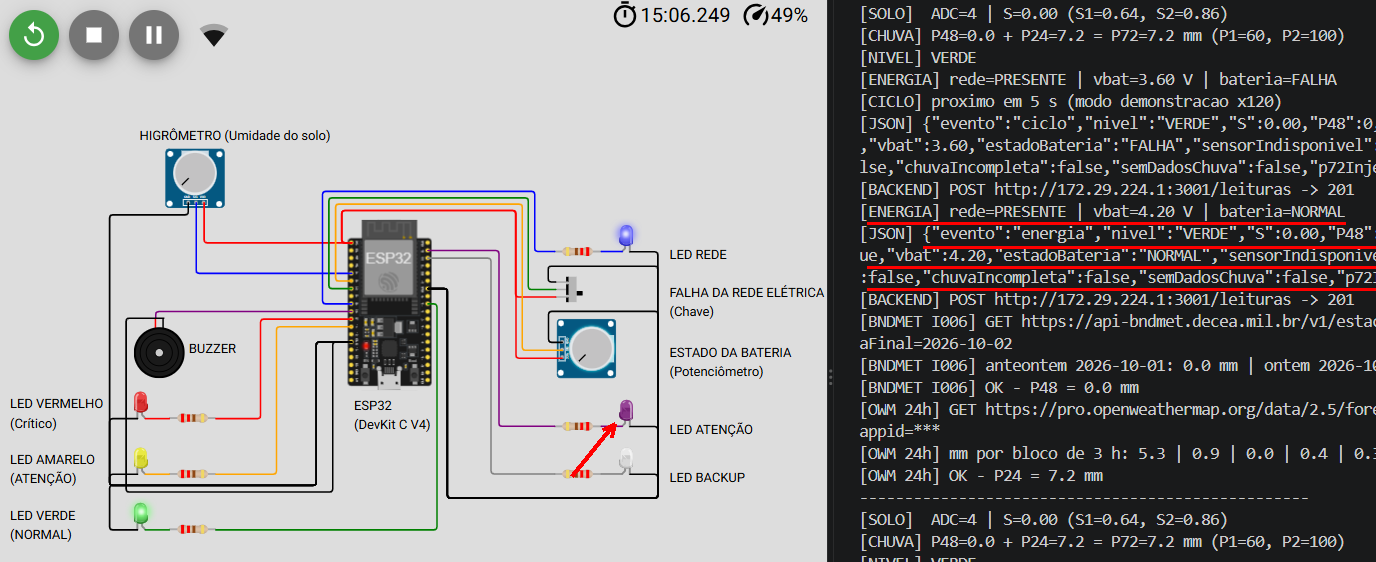
\includegraphics[width=\textwidth]{figures/cap5/E04c_bateria_substituida.png}}
\caption{Caso E04c na simulação: bateria em 4,20\,V e retorno ao estado normal}
\label{fig:res-e04c}
\fonte{Autora, 2026.}
\end{figure}

\begin{figure}[H]
\centering
\fbox{\includegraphics[width=\textwidth,trim=232 1102 236 0,clip]{figures/cap5/W13_painel_E04b_falha.pdf}}
\caption{Painel no caso E04b: rede presente e bateria com falha (``Falha: substituir'')}
\label{fig:res-w13}
\fonte{Autora, 2026.}
\end{figure}

Cada mudança de energia gerou um evento no \textit{backend} e um e-mail
automático aos administradores, registrados no painel
(\autoref{fig:res-w18}, na \autoref{sec:res-web}).

% -------------------------------------------------------------
\subsection{Autonomia Calculada}
\label{subsec:res-autonomia}
% -------------------------------------------------------------

A autonomia da bateria não foi ensaiada: o simulador não reproduz o
consumo, e a bateria não foi montada no protótipo físico. A
\autoref{tab:autonomia} reúne os valores teóricos obtidos com as
equações e a corrente da \autoref{subsec:energia}.

\begin{table}[htb]
\centering
\caption{Autonomia da alimentação redundante (valores teóricos, não medidos)}
\label{tab:autonomia}
\small
\begin{tabular}{p{7.0cm}p{3.2cm}p{3.8cm}}
\hline
\textbf{Grandeza} & \textbf{Valor calculado} & \textbf{Origem} \\
\hline
Corrente na placa em supervisão & 167\,mA & \autoref{tab:consumo} \\
Corrente na placa em alarme & 202\,mA & \autoref{tab:consumo} \\
Capacidade na entrada da placa ($C_{\mathrm{carga}}$) & 4870,2\,mAh & \autoref{eq:cap-carga} \\
Capacidade necessária na bateria ($C_{\mathrm{bat}}$) & 7816\,mAh & \autoref{eq:cap-celula} \\
Células NCR18650B em paralelo ($n$) & 3 (9600\,mAh) & \autoref{eq:num-celulas} \\
Corrente na bateria em supervisão & 268,0\,mA & \autoref{eq:cap-celula}, com 167\,mA \\
Corrente na bateria em alarme & 324,2\,mA & \autoref{eq:cap-celula}, com 202\,mA \\
Carga usada em 24\,h de supervisão e 15\,min de alarme & 6513\,mAh (68\% de 9600\,mAh) & $268{,}0 \times 24 + 324{,}2 \times 0{,}25$ \\
Autonomia em supervisão, sem margem & cerca de 36\,h & $9600 / 268{,}0$ \\
Autonomia em alarme contínuo, sem margem & cerca de 29,6\,h & $9600 / 324{,}2$ \\
Operação restante a partir de 3,3\,V (bateria baixa) & cerca de 5\,h & \autoref{subsec:energia} \\
Operação restante a partir de 3,0\,V (bateria crítica) & cerca de 1,4\,h & \autoref{subsec:energia} \\
Tempo máximo de recarga ($T_{\mathrm{carga}}$) & 19,5\,h (585\,s na simulação) & \autoref{eq:tempo-carga} \\
\hline
\end{tabular}
\fonte{Autora, 2026, com base nas \autoref{eq:cap-carga} a \autoref{eq:tempo-carga}, na \autoref{tab:consumo} e em \citeonline{panasonic_ncr18650b}.}
\end{table}

Pelo cálculo, as três células atendem ao requisito de 24~horas de
supervisão e 15~minutos de alarme \cite[item~5.3]{cbmmg2017it14} com
cerca de 32\% da capacidade restante. Esses valores dependem das
correntes adotadas dos \textit{datasheets} e não foram verificados em
ensaio.

Na simulação, foram verificados apenas a lógica dos estados de energia
e os avisos correspondentes (\autoref{tab:res-energia}), e não a
duração da bateria.

% =============================================================
\section{Protótipo Físico}
\label{sec:res-fisico}
% =============================================================

Os casos F01 a F08 seguem a \autoref{tab:casos-fisico}, com o
\textit{firmware} do ESP8266 gravado pela Arduino IDE e o monitor serial
na porta COM3. Os mesmos comandos de teste da simulação foram usados, e
o modo de demonstração também reduziu os intervalos entre ciclos.

A \autoref{fig:res-f00-foto} mostra o protótipo em operação, alimentado
pela porta USB-C, com o LED azul aceso no nível VERDE. A umidade em
torno da sonda foi variada mantendo-a fora da água, com as pontas na
água ou imersa em água em um recipiente; essas condições não
representam o maciço de uma barragem.

\begin{figure}[H]
\centering
\fbox{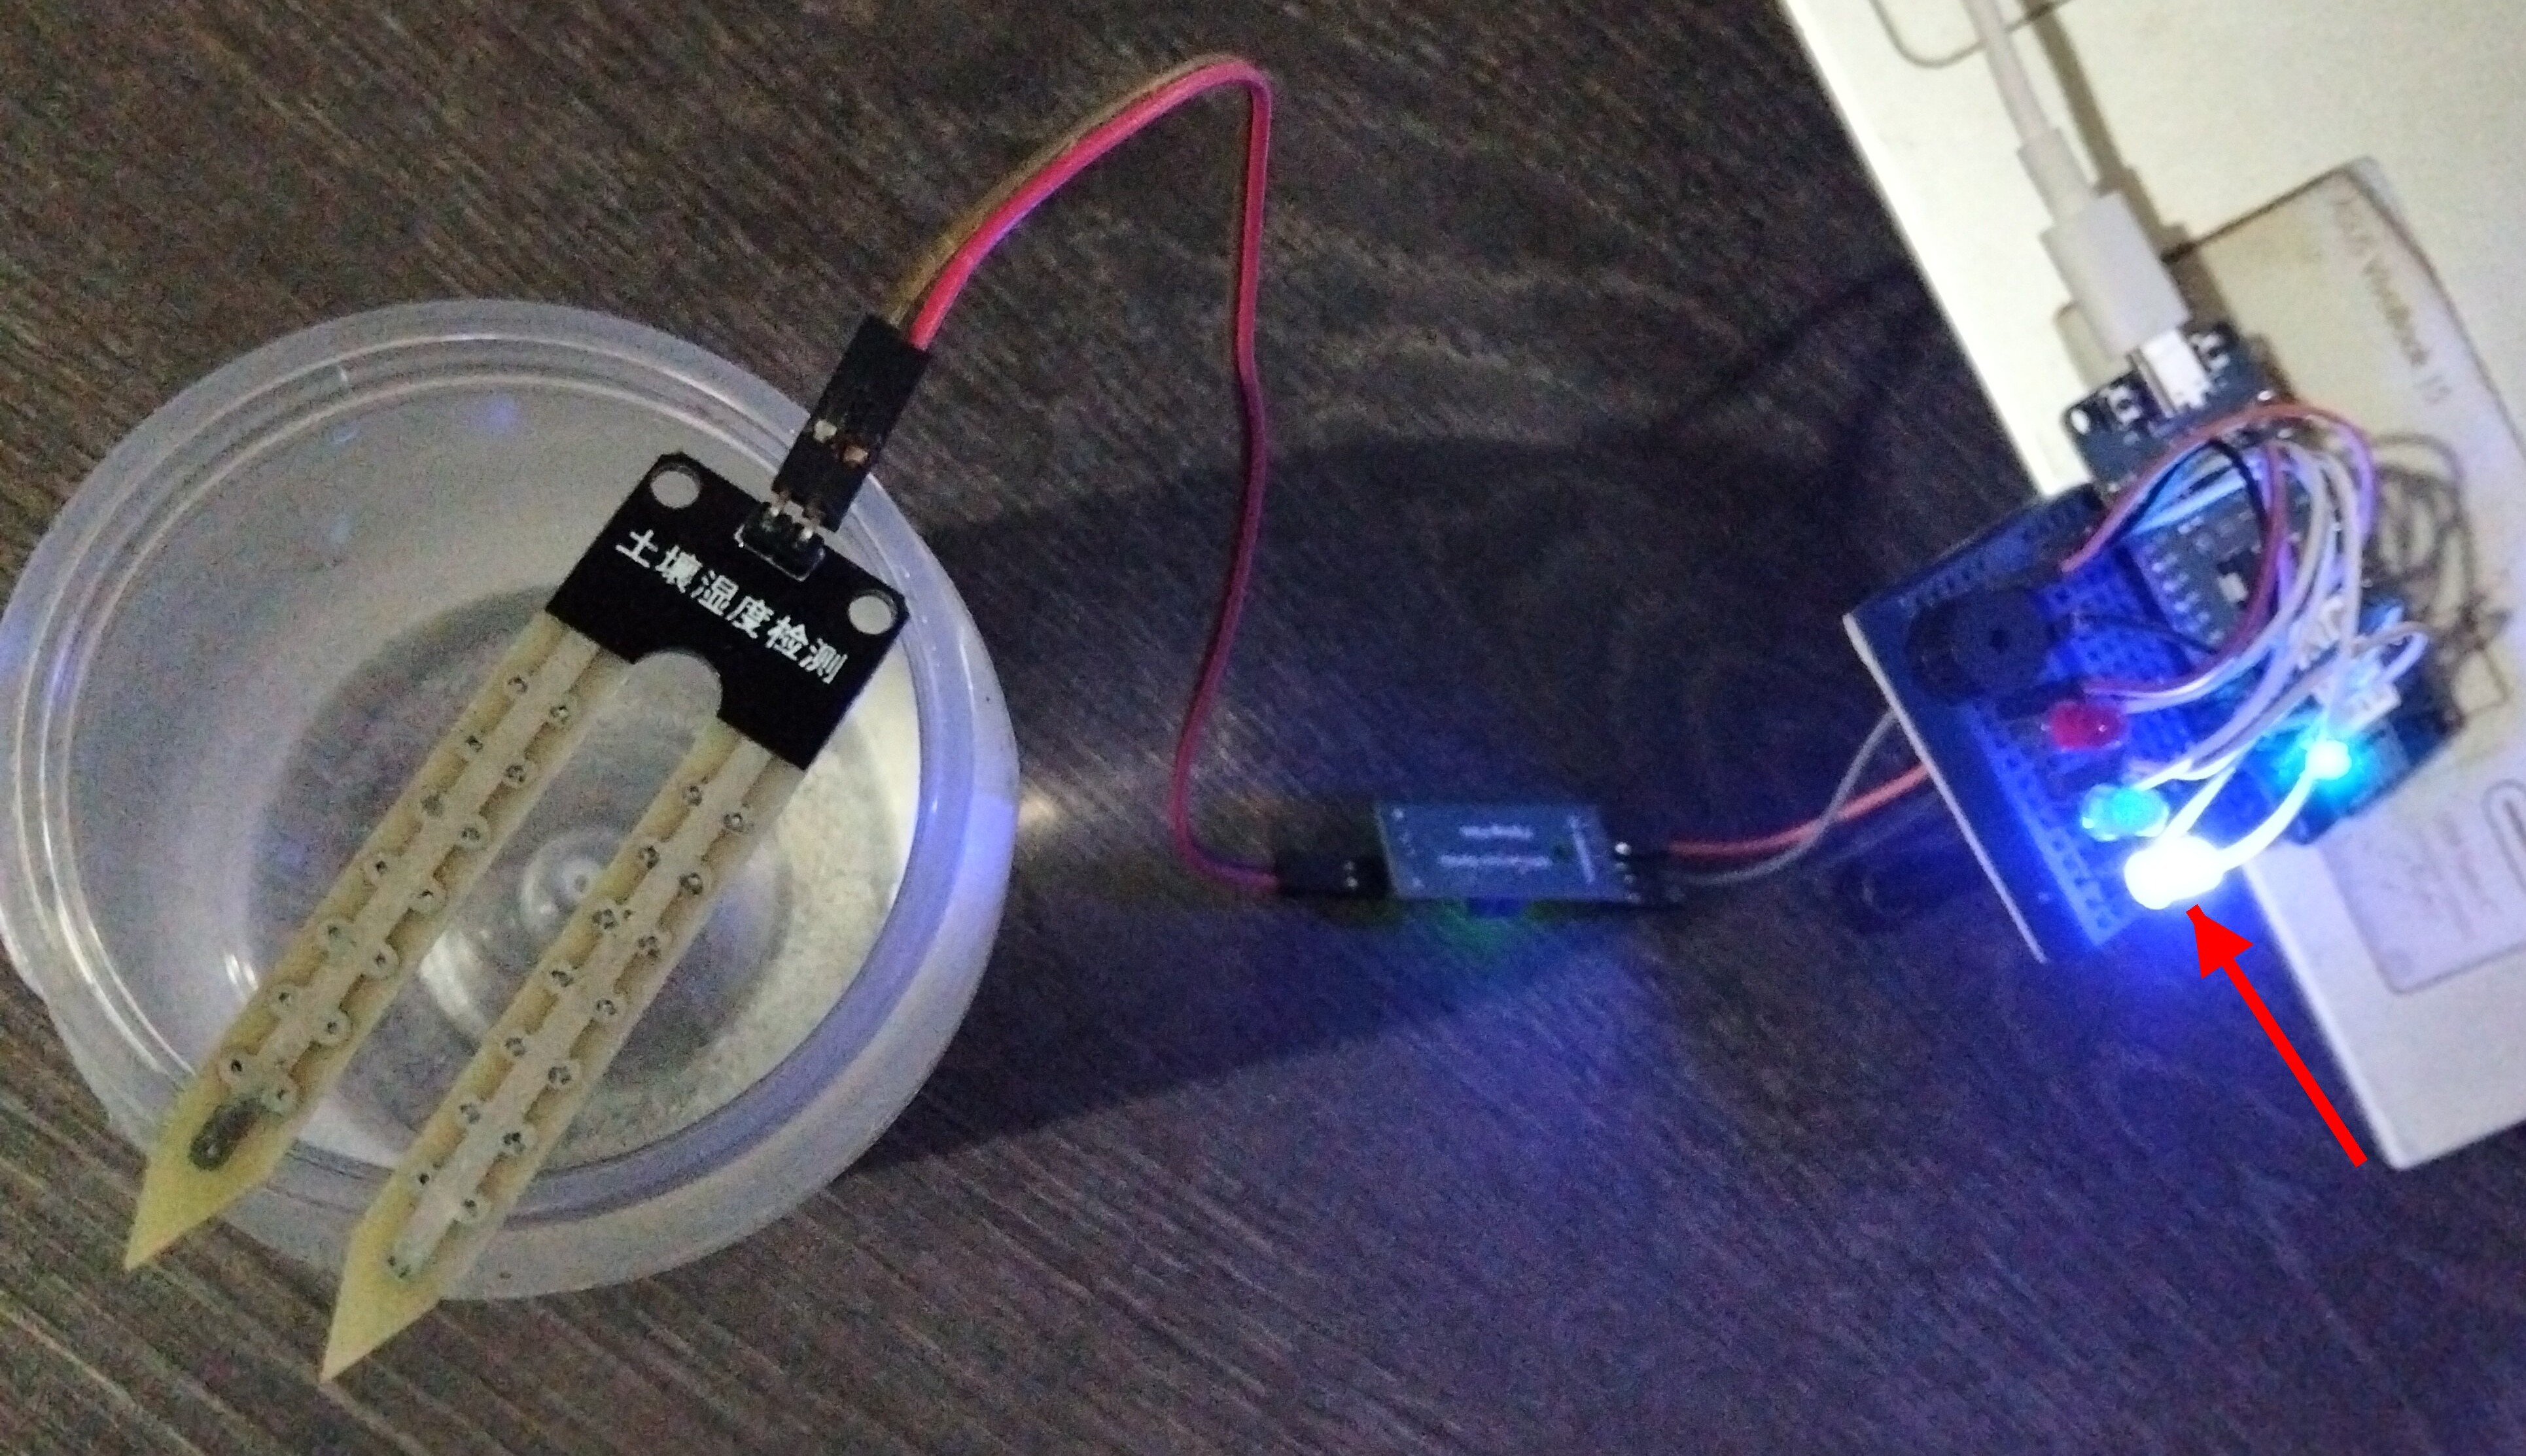
\includegraphics[width=0.85\textwidth]{figures/cap5/F00_firmware.jpg}}
\caption{Protótipo físico em operação, com a sonda imersa em água e o LED azul aceso (nível VERDE)}
\label{fig:res-f00-foto}
\fonte{Autora, 2026.}
\end{figure}

\paragraph*{Calibração}

Antes dos casos, o higrômetro foi calibrado pelos comandos
\texttt{calibrar seco}, com a sonda seca e fora da água, e
\texttt{calibrar sat}, com a sonda imersa em água. As leituras gravadas
foram $L_{\mathrm{seco}} = 886$ e $L_{\mathrm{sat}} = 233$, usadas na
\autoref{eq:saturacao} (\autoref{fig:res-f00}).

\begin{figure}[H]
\centering
\fbox{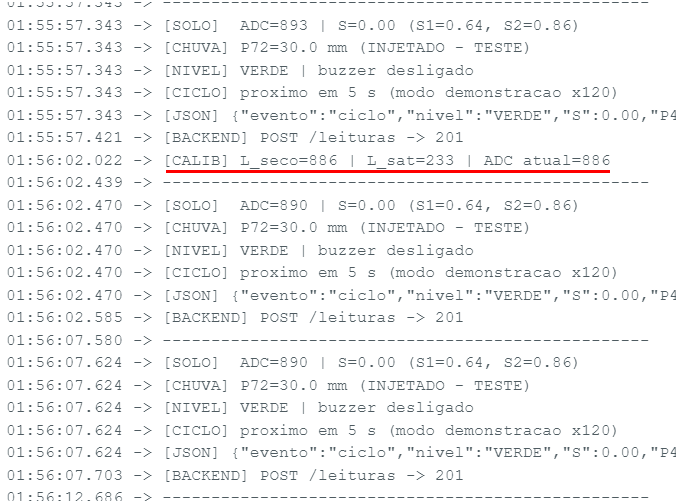
\includegraphics[width=\textwidth]{figures/cap5/F00_calibracao.png}}
\caption{Calibração do higrômetro no protótipo físico: $L_{\mathrm{seco}} = 886$ e $L_{\mathrm{sat}} = 233$}
\label{fig:res-f00}
\fonte{Autora, 2026.}
\end{figure}

A \autoref{tab:res-fisico} resume os resultados. Como a umidade em torno
da sonda não pode ser ajustada com precisão, a saída esperada foi
definida pela faixa do $S$ lido (\autoref{tab:matriz}).

\begin{table}[htb]
\centering
\caption{Resultados dos casos no protótipo físico}
\label{tab:res-fisico}
\small
\begin{tabular}{p{0.9cm}p{5.0cm}p{3.6cm}p{4.6cm}}
\hline
\textbf{Caso} & \textbf{Entrada observada} & \textbf{Saída esperada} & \textbf{Saída observada} \\
\hline
F01 & Sonda fora da água, $S$ de 0,25 a 0,30; $P_{72} = 120$\,mm & VERDE & VERDE; LED azul; \textit{buzzer} desligado \\
F02 & Pontas da sonda na água, $S$ de 0,77 a 0,81; $P_{72} = 80$\,mm & AMARELO & AMARELO; LED amarelo; \textit{buzzer} desligado \\
F03 & Sonda imersa, $S$ de 0,93 a 0,95; $P_{72} = 120$\,mm & VERMELHO; \textit{buzzer} acionado & VERMELHO; LED vermelho; \textit{buzzer} ligado \\
F04 & Sonda imersa, $S$ de 0,93 a 0,94; $P_{72} = 30$\,mm & VERDE & VERDE; LED azul \\
F05 & Sonda desconectada (leitura 1023); $P_{72} = 80$\,mm & AMARELO, pela chuva & AMARELO; higrômetro indisponível; LED amarelo \\
F06 & Sonda imersa, $S = 1{,}00$; sem dados de chuva & AMARELO (caso especial) & AMARELO; ``sem dados de chuva''; LED amarelo \\
F07 & APIs reais; um dia sem registro; mínimo de 1,3\,mm & Mínimo tratado como falta de dados de chuva & VERDE com $S$ de 0,00 e 0,83; AMARELO com $S = 1{,}00$ \\
F08 & Sonda imersa, $S = 1{,}00$; dados incompletos, mínimo de 120\,mm & VERMELHO; \textit{buzzer} acionado & VERMELHO; LED vermelho; \textit{buzzer} ligado \\
\hline
\end{tabular}
\fonte{Autora, 2026, com base nos registros do protótipo físico.}
\end{table}

\paragraph*{Caso F01 --- sonda fora da água e $P_{72}$ alto}

Entrada: sonda fora da água ($S$ de 0,25 a 0,30) e $P_{72} = 120$\,mm.
Saída esperada: VERDE, com o LED azul. Saída observada:
``\texttt{VERDE | buzzer desligado}'' e LED azul aceso
(\autoref{fig:res-f01-foto} e \autoref{fig:res-f01-serial}).

\begin{figure}[H]
\centering
\fbox{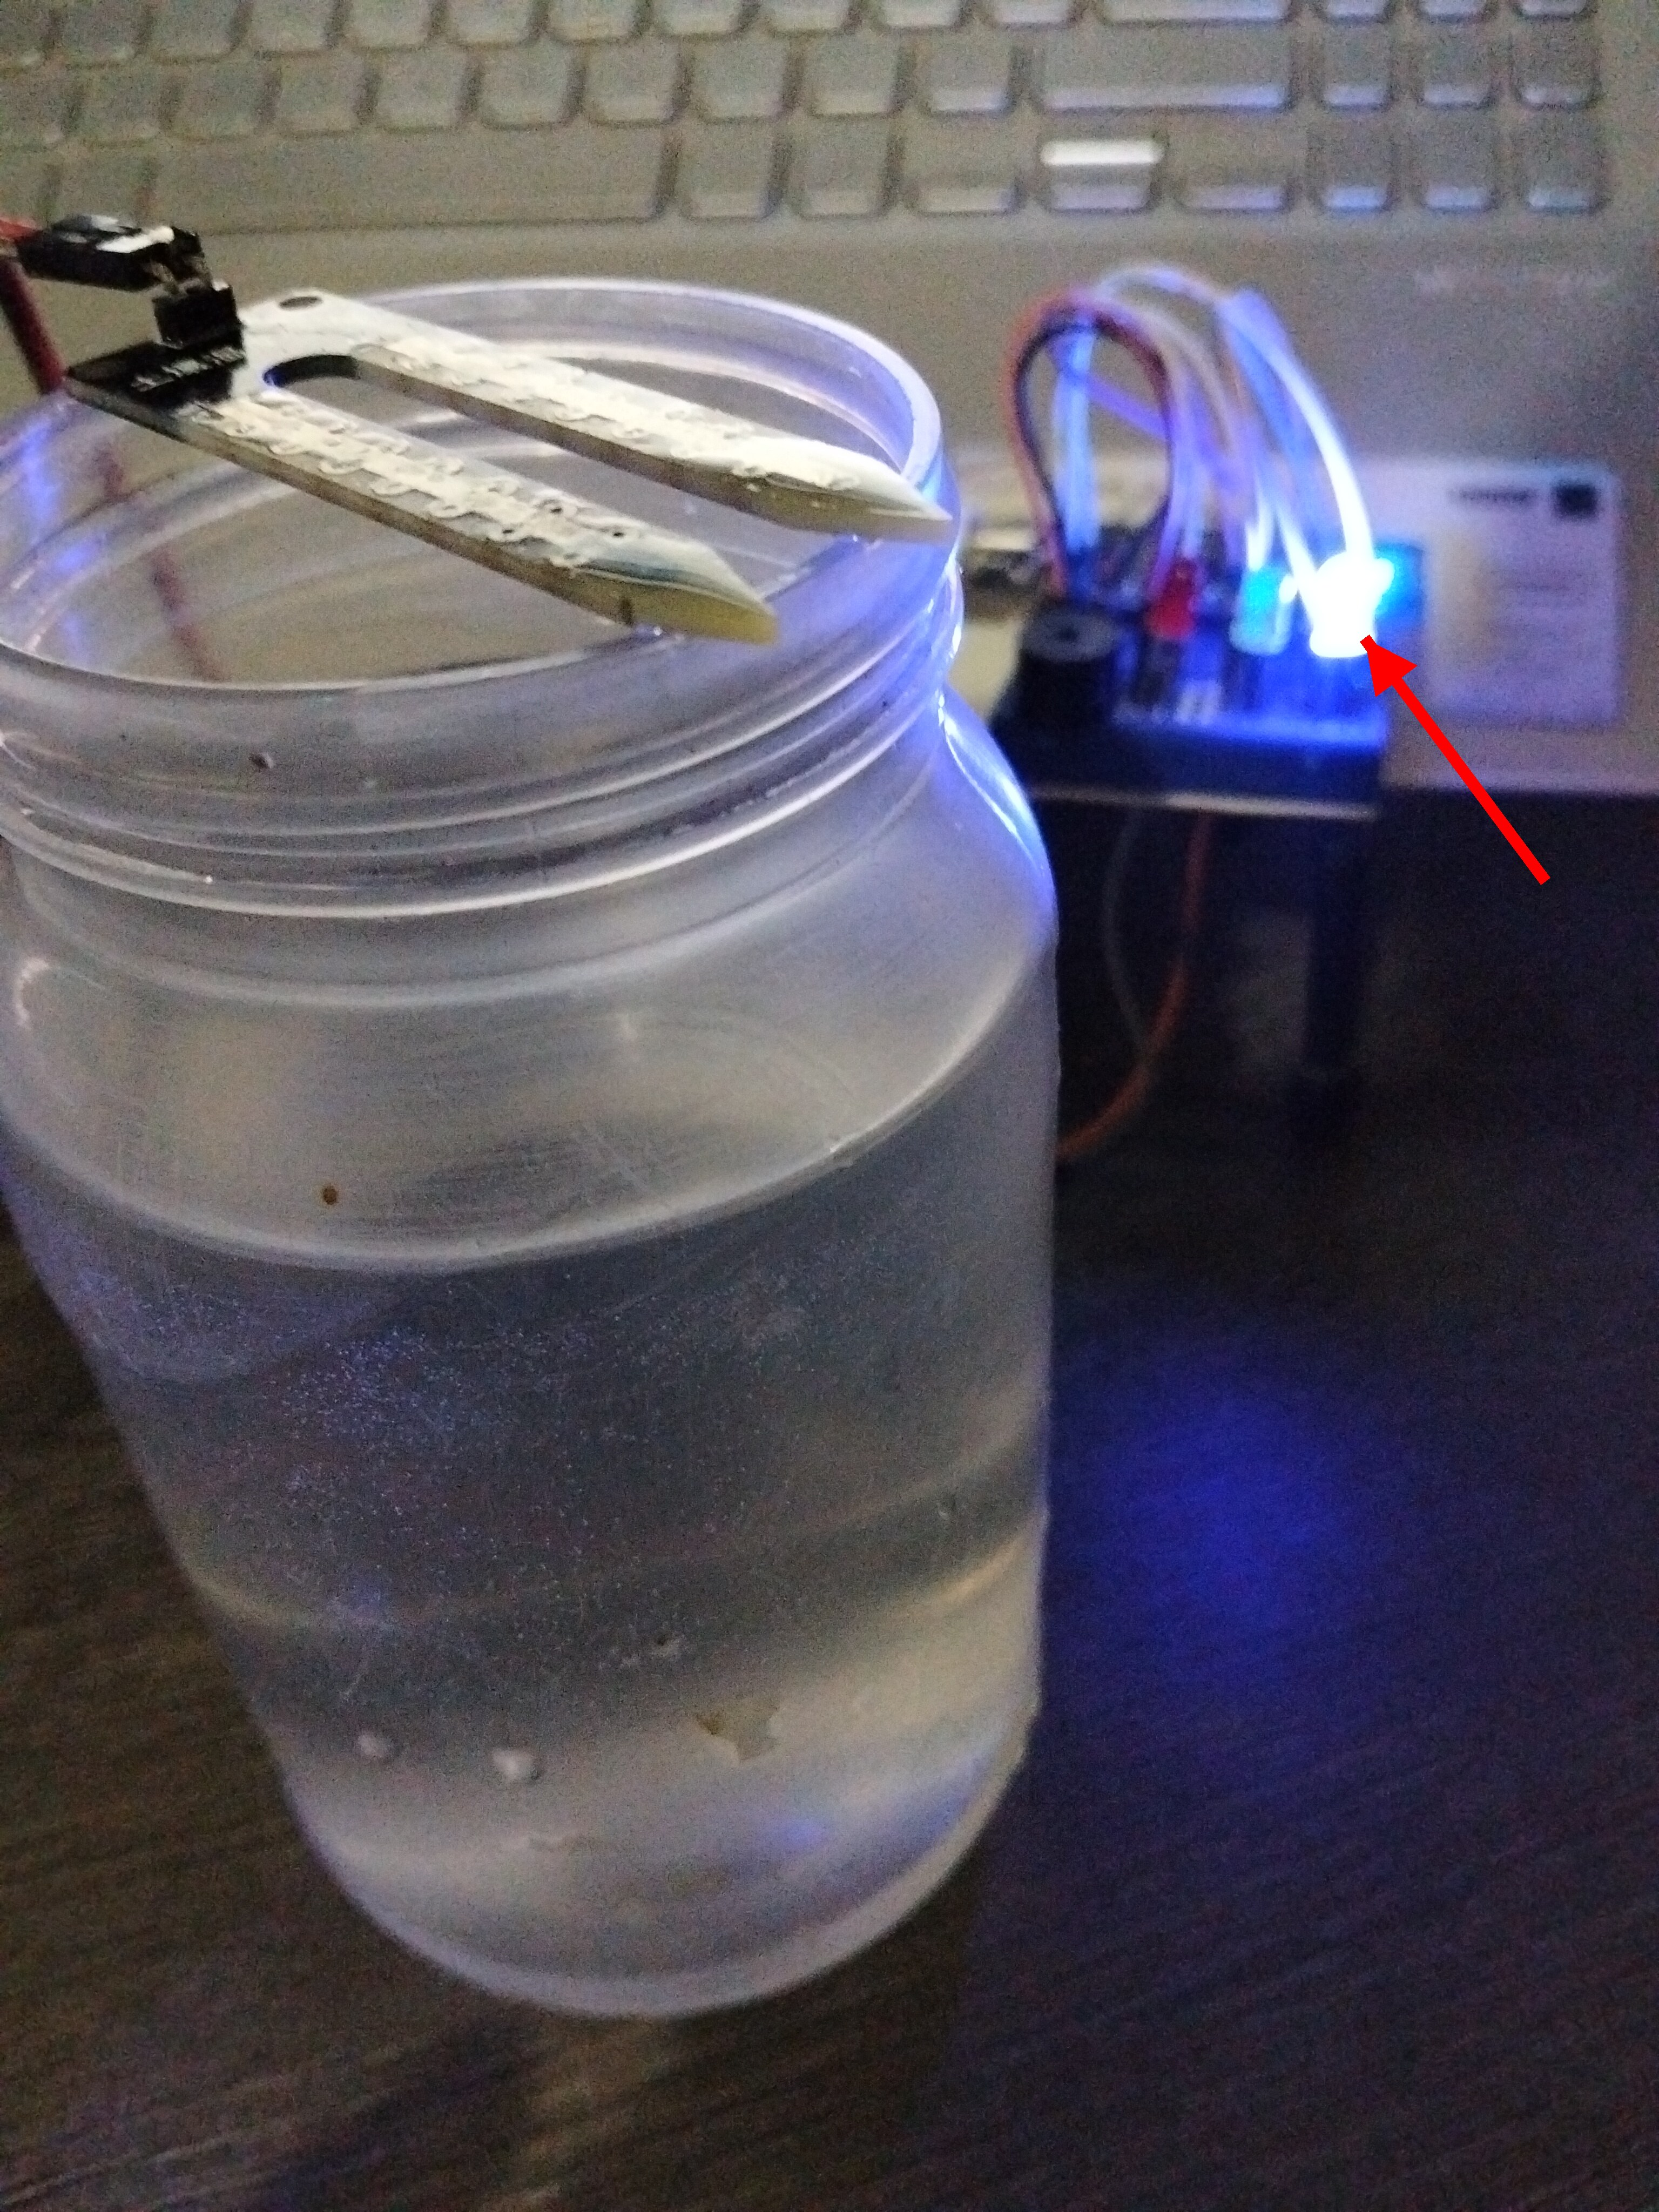
\includegraphics[height=0.42\textheight,keepaspectratio]{figures/cap5/F01_foto.jpg}}
\caption{Caso F01 no protótipo físico: sonda fora da água e LED azul aceso (VERDE)}
\label{fig:res-f01-foto}
\fonte{Autora, 2026.}
\end{figure}

\begin{figure}[H]
\centering
\fbox{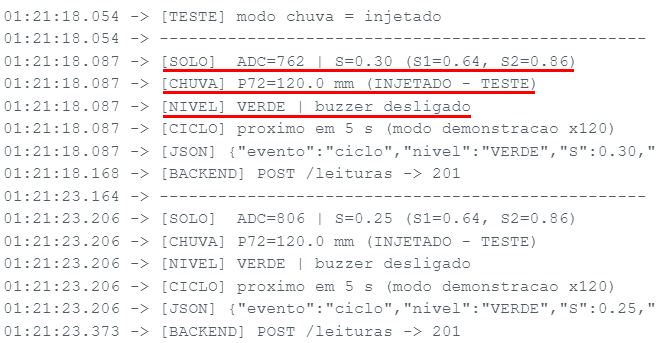
\includegraphics[width=\textwidth]{figures/cap5/F01_serial.png}}
\caption{Caso F01: monitor serial com $S$ de 0,25 a 0,30 e $P_{72} = 120$\,mm, nível VERDE}
\label{fig:res-f01-serial}
\fonte{Autora, 2026.}
\end{figure}

\paragraph*{Caso F02 --- sonda com as pontas na água e $P_{72}$ moderado}

Entrada: sonda com apenas as pontas imersas em água ($S$ de 0,77 a
0,81, entre $S_1$ e $S_2$) e $P_{72} = 80$\,mm. Saída esperada:
AMARELO. Saída observada: ``\texttt{AMARELO | buzzer desligado}'' e LED
amarelo aceso (\autoref{fig:res-f02-foto} e
\autoref{fig:res-f02-serial}).

\begin{figure}[H]
\centering
\fbox{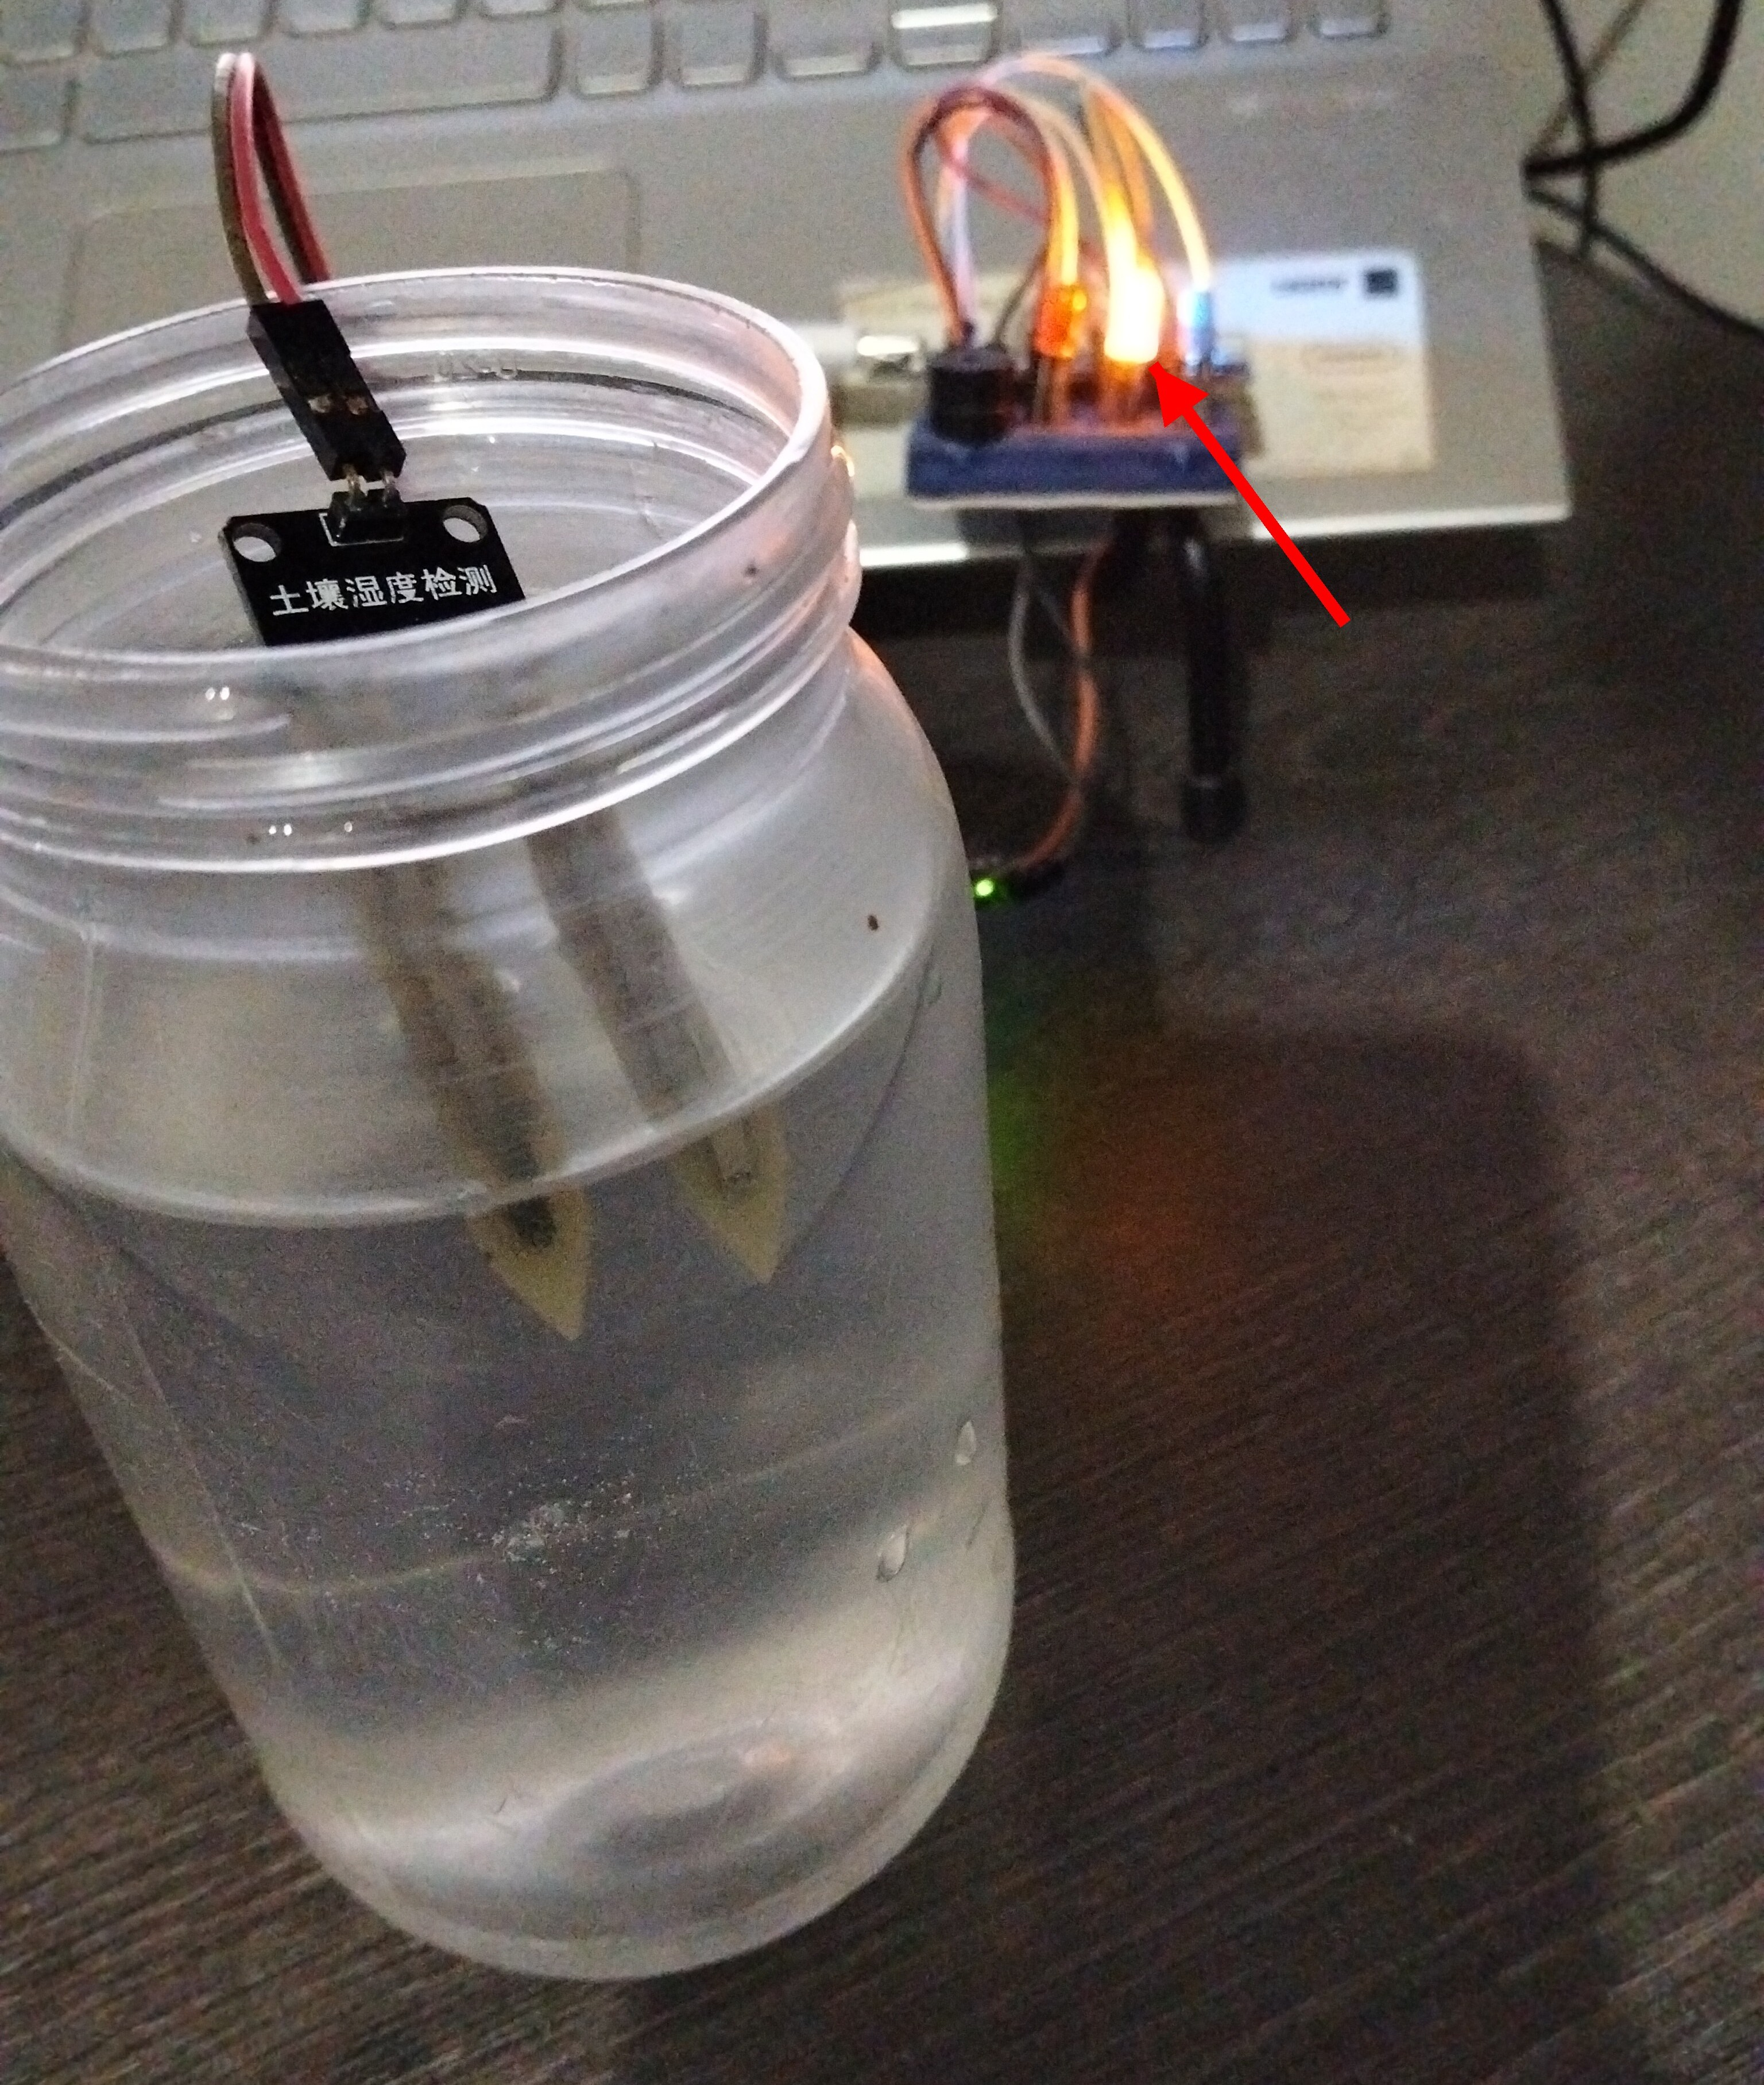
\includegraphics[height=0.42\textheight,keepaspectratio]{figures/cap5/F02_foto.jpg}}
\caption{Caso F02 no protótipo físico: sonda com as pontas na água e LED amarelo aceso (AMARELO)}
\label{fig:res-f02-foto}
\fonte{Autora, 2026.}
\end{figure}

\begin{figure}[H]
\centering
\fbox{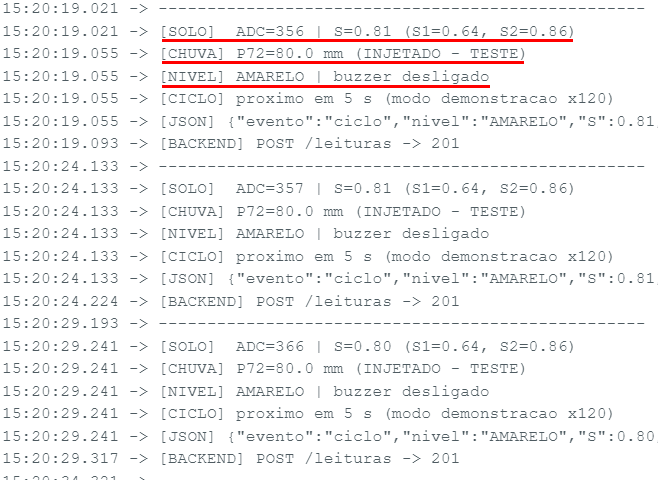
\includegraphics[width=\textwidth]{figures/cap5/F02_serial.png}}
\caption{Caso F02: monitor serial com $S = 0{,}81$ e $P_{72} = 80$\,mm, nível AMARELO}
\label{fig:res-f02-serial}
\fonte{Autora, 2026.}
\end{figure}

\paragraph*{Caso F03 --- sonda imersa e $P_{72}$ alto}

Entrada: sonda imersa ($S$ de 0,93 a 0,95) e $P_{72} = 120$\,mm. Saída
esperada: VERMELHO, com o \textit{buzzer} acionado. Saída observada:
``\texttt{VERMELHO | buzzer LIGADO}'', LED vermelho aceso e
\textit{buzzer} TMB-12A03 soando (\autoref{fig:res-f03-foto} e
\autoref{fig:res-f03-serial}).

\begin{figure}[H]
\centering
\fbox{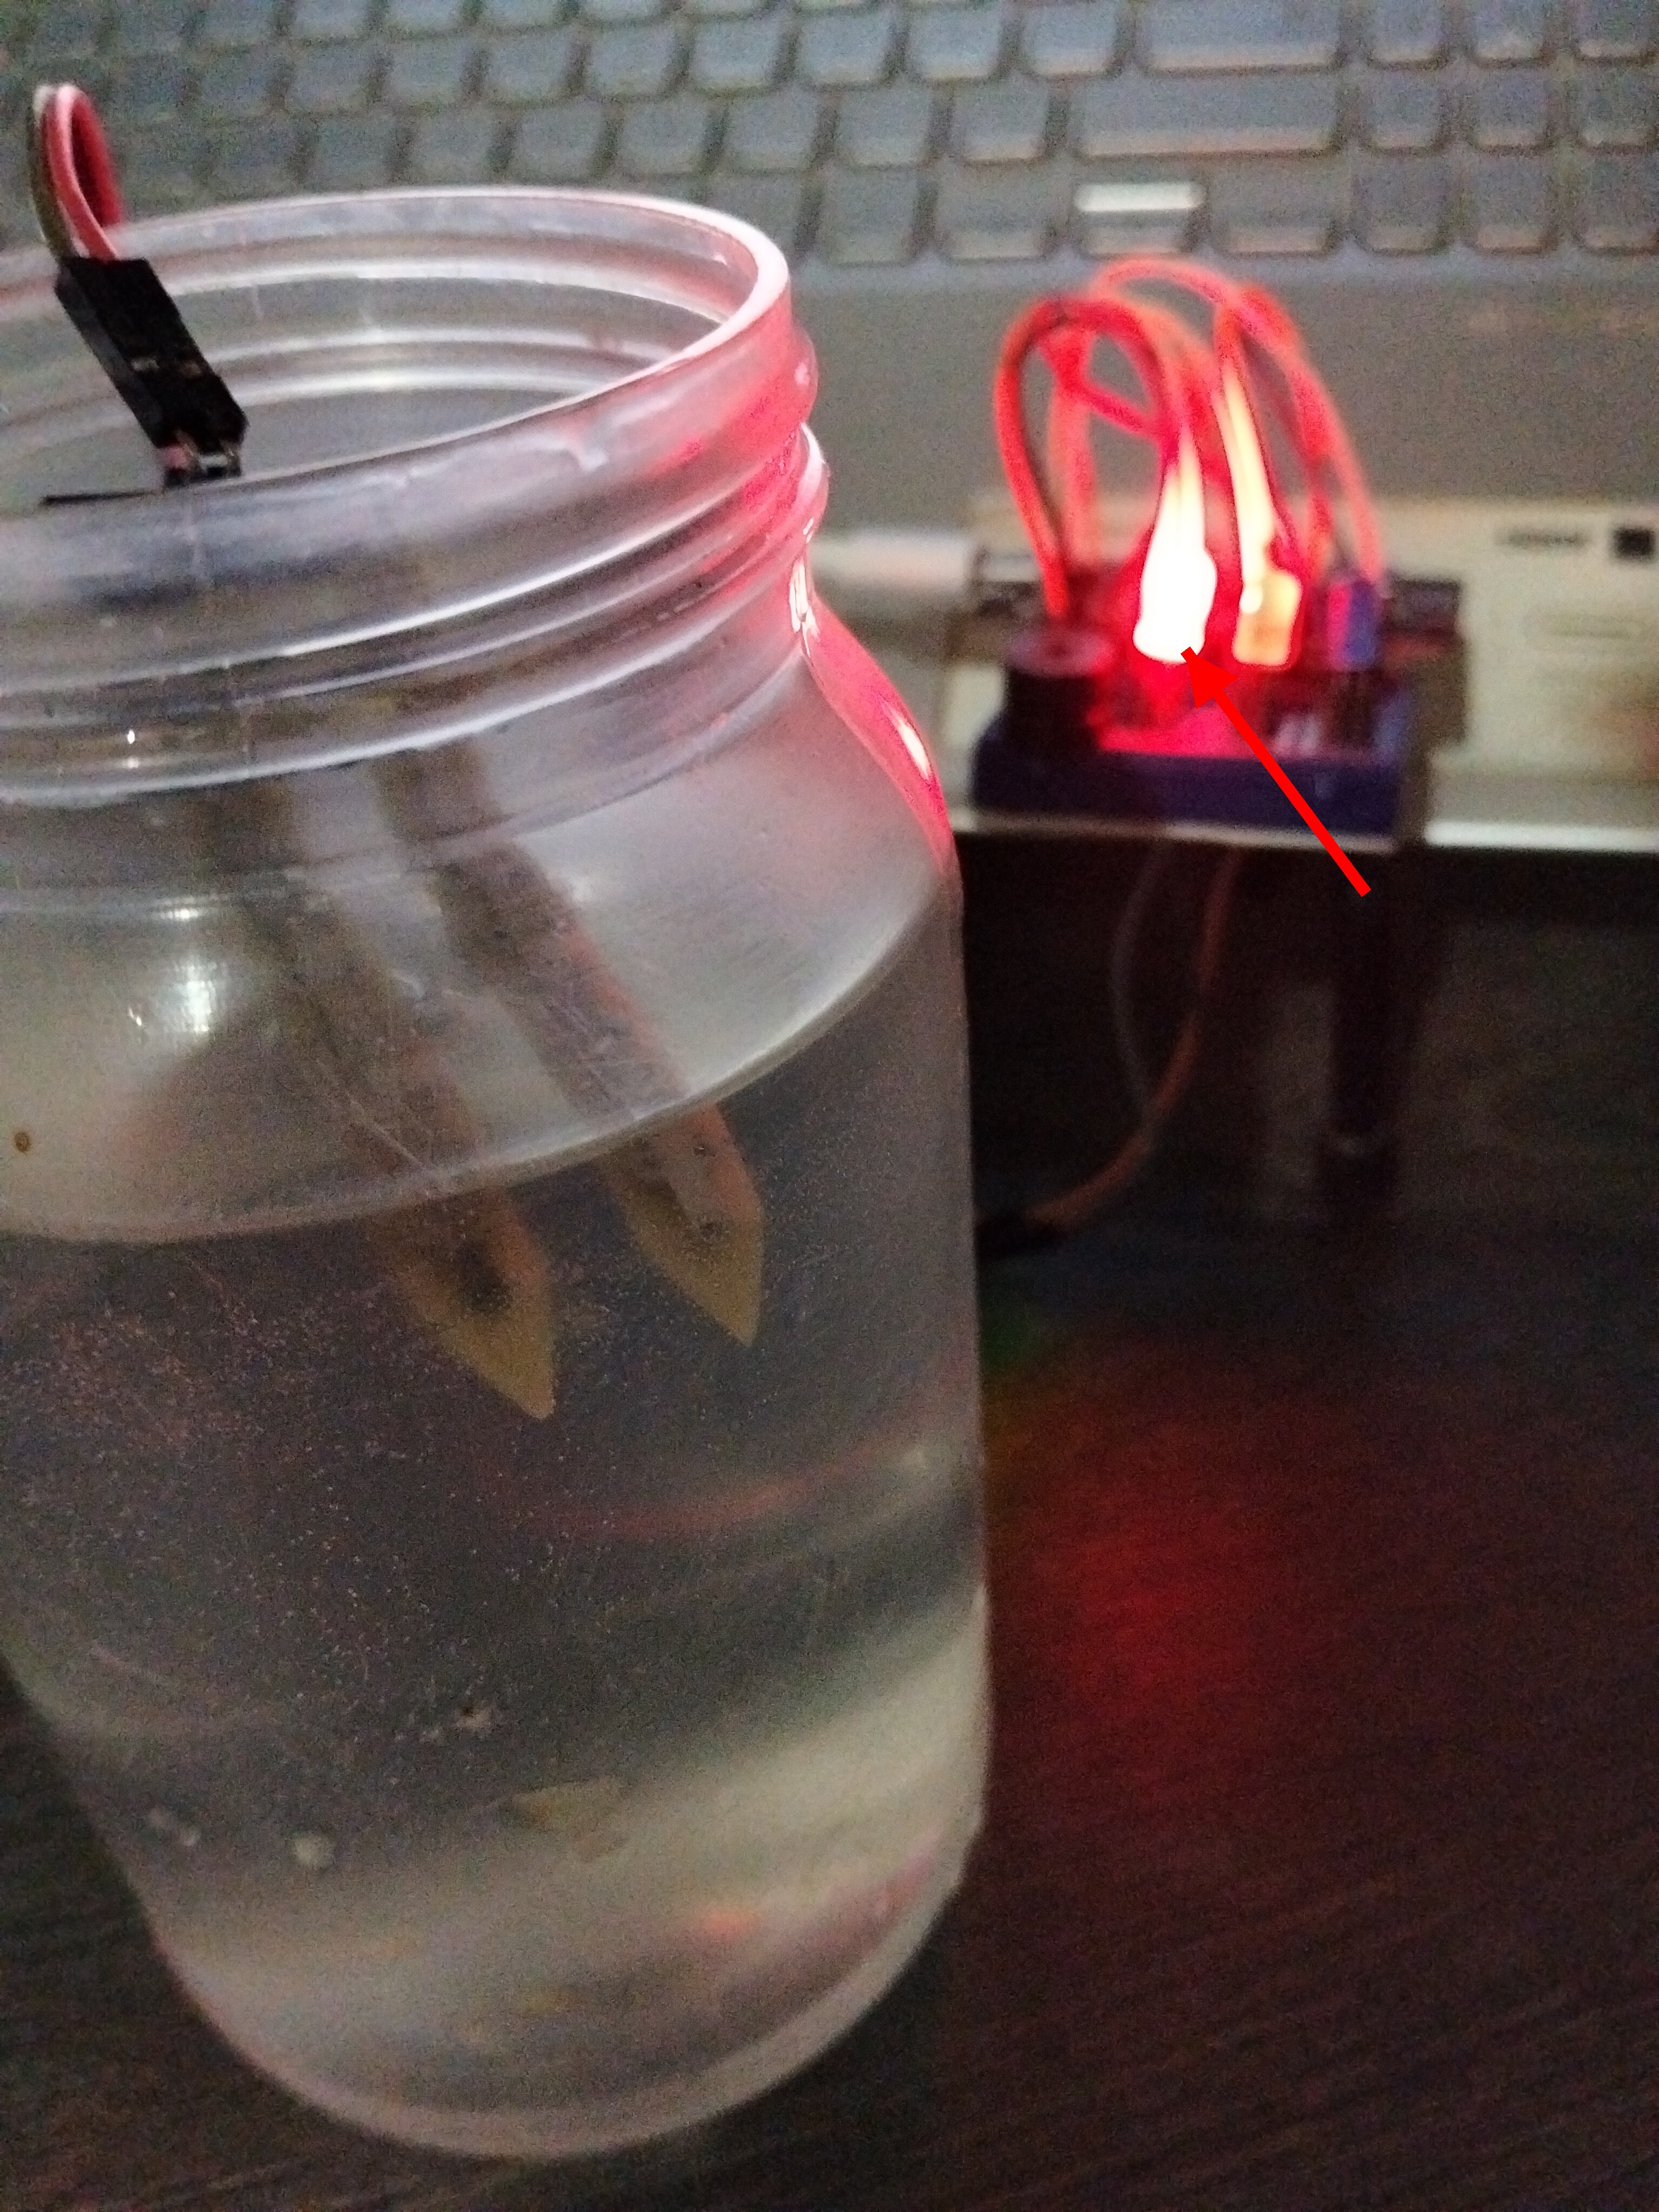
\includegraphics[height=0.42\textheight,keepaspectratio]{figures/cap5/F03_foto.jpg}}
\caption{Caso F03 no protótipo físico: sonda imersa e LED vermelho aceso (VERMELHO)}
\label{fig:res-f03-foto}
\fonte{Autora, 2026.}
\end{figure}

\begin{figure}[H]
\centering
\fbox{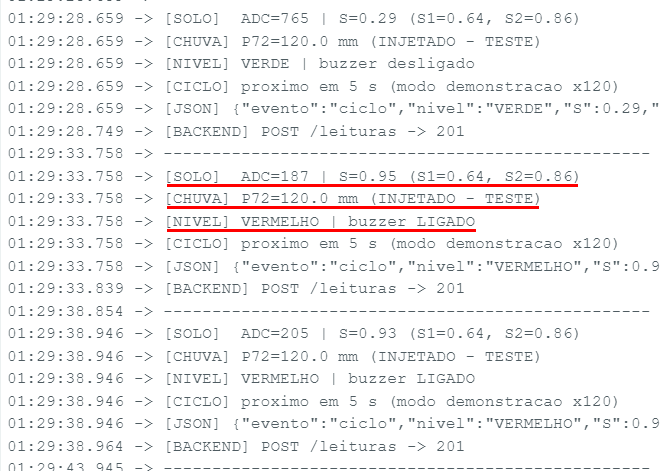
\includegraphics[width=\textwidth]{figures/cap5/F03_serial.png}}
\caption{Caso F03: monitor serial com $S$ de 0,93 a 0,95 e $P_{72} = 120$\,mm, nível VERMELHO e \textit{buzzer} ligado}
\label{fig:res-f03-serial}
\fonte{Autora, 2026.}
\end{figure}

\paragraph*{Caso F04 --- sonda imersa e $P_{72}$ baixo}

Entrada: sonda imersa ($S$ de 0,93 a 0,94) e $P_{72} = 30$\,mm. Saída
esperada: VERDE. Saída observada: ``\texttt{VERDE | buzzer
desligado}'' e LED azul aceso (\autoref{fig:res-f04-foto} e
\autoref{fig:res-f04-serial}).

\begin{figure}[H]
\centering
\fbox{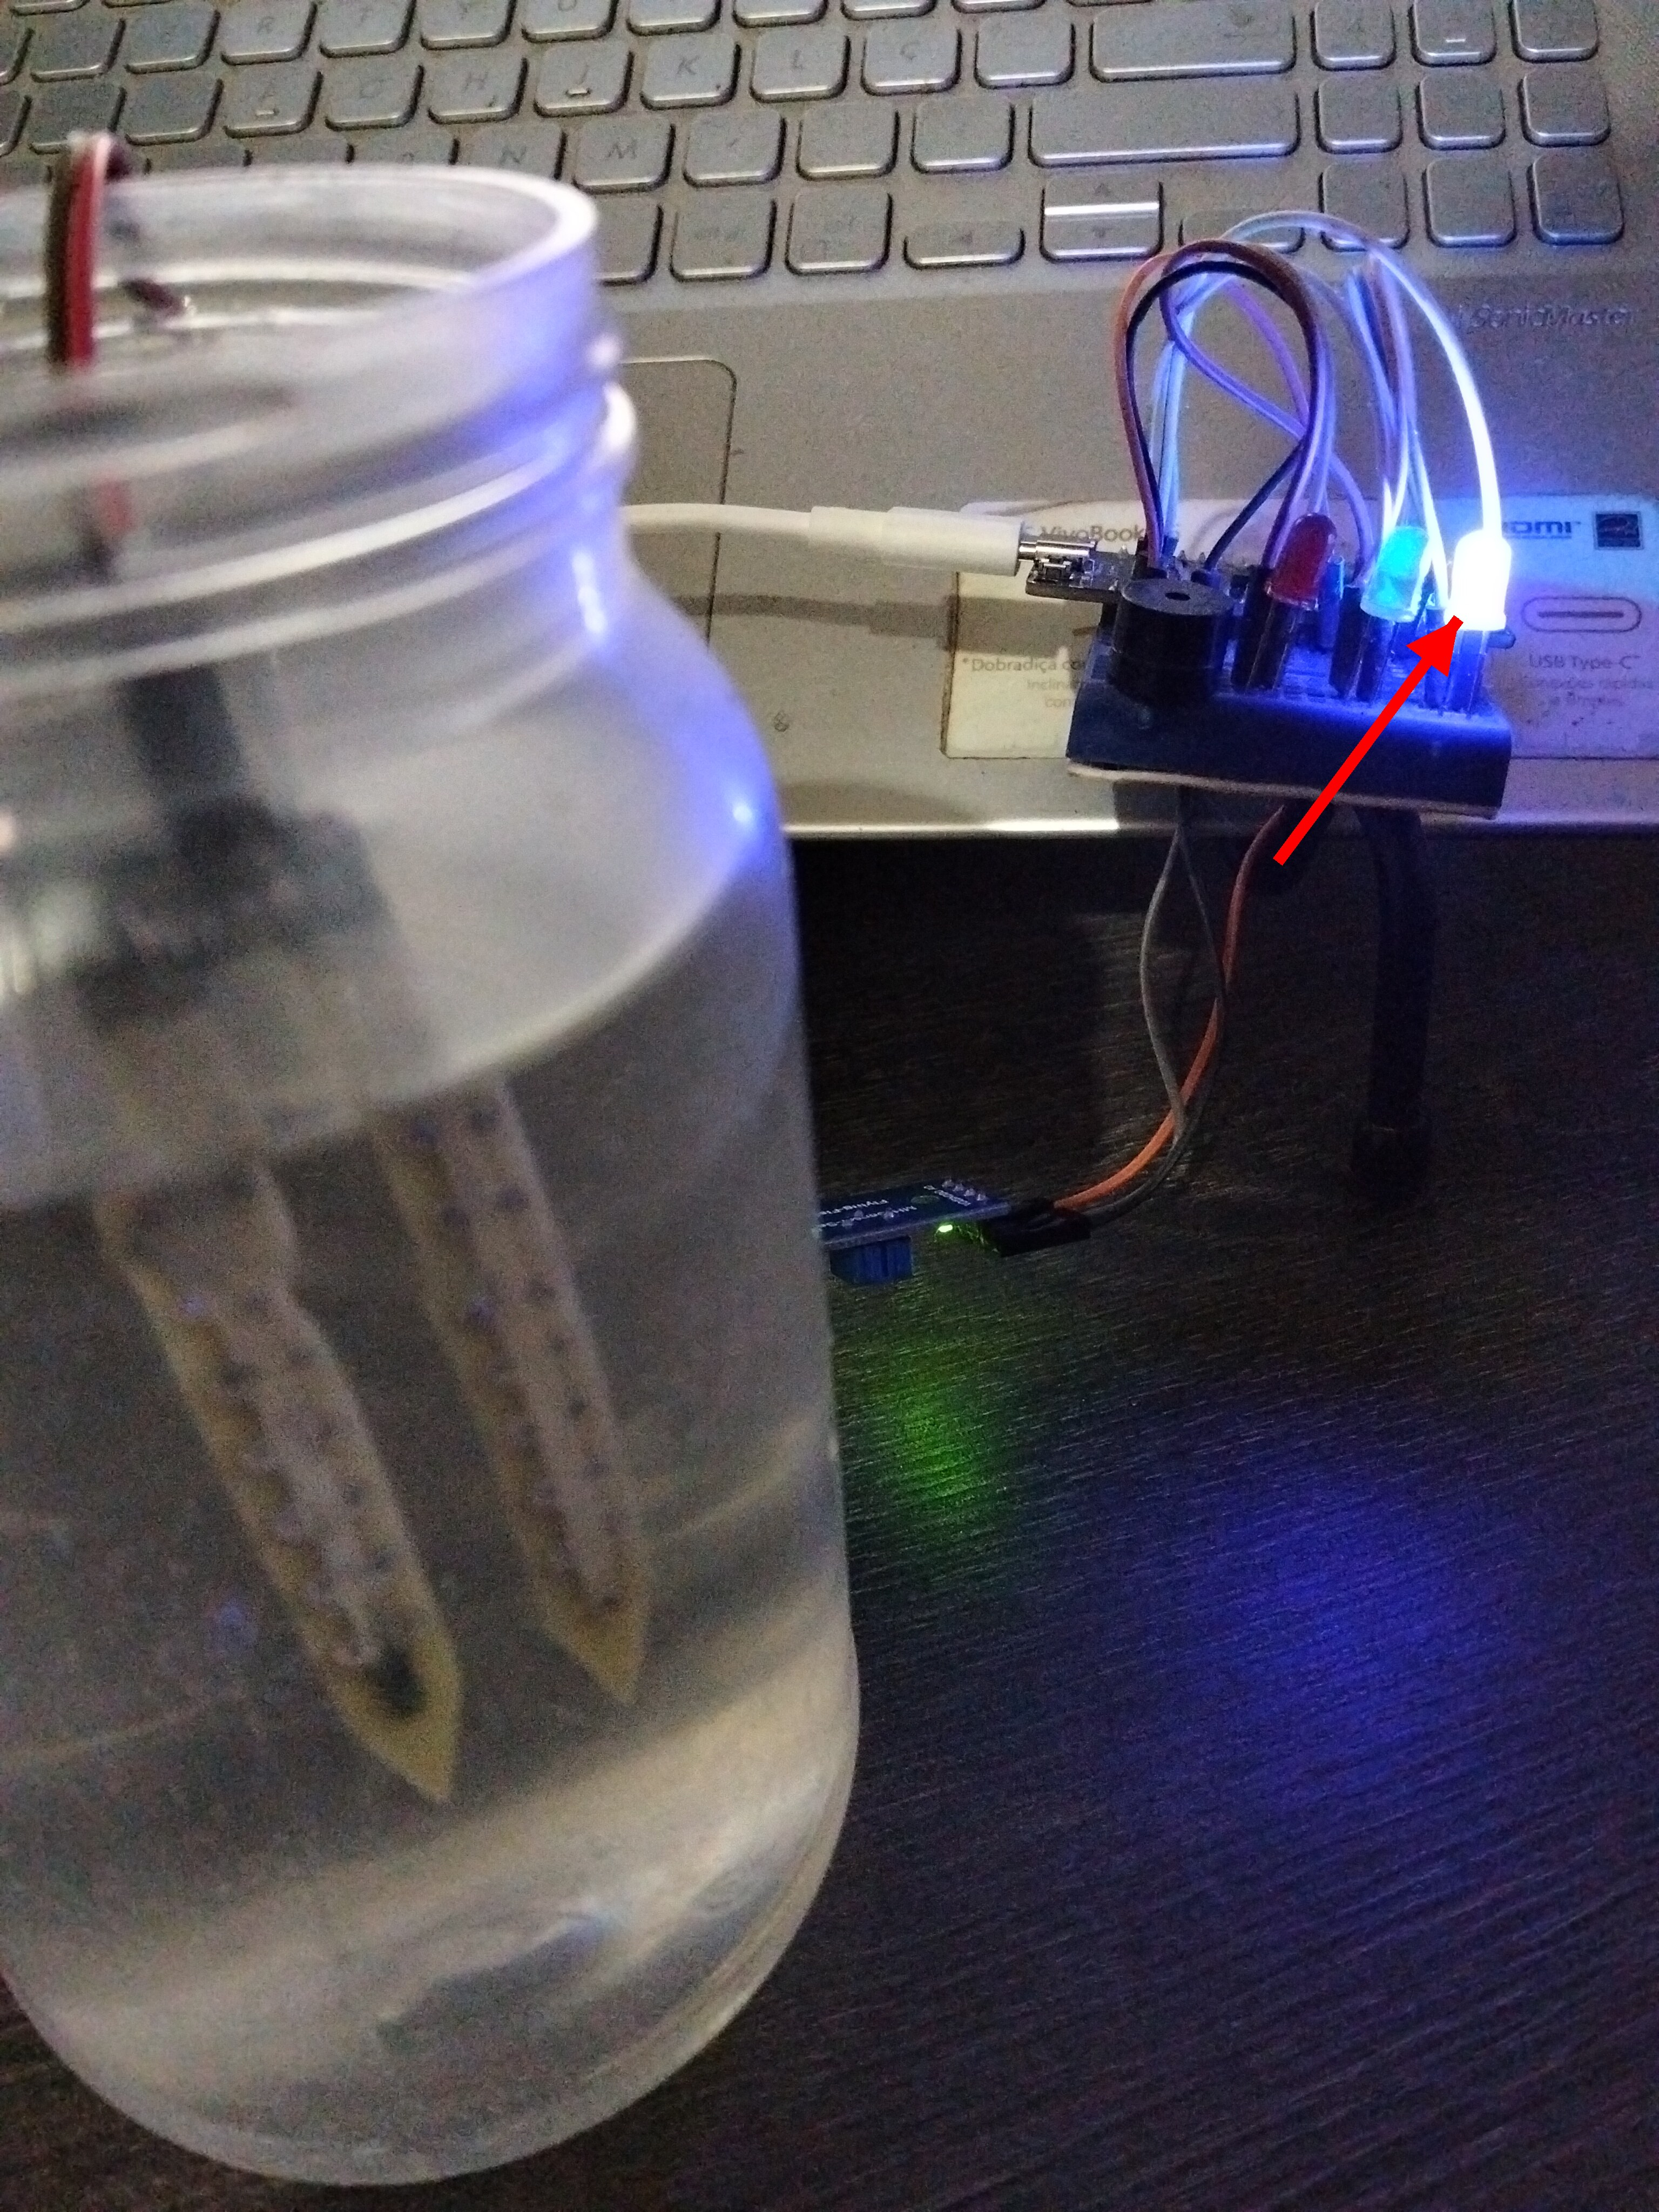
\includegraphics[height=0.42\textheight,keepaspectratio]{figures/cap5/F04_foto.jpg}}
\caption{Caso F04 no protótipo físico: sonda imersa e LED azul aceso (VERDE)}
\label{fig:res-f04-foto}
\fonte{Autora, 2026.}
\end{figure}

\begin{figure}[H]
\centering
\fbox{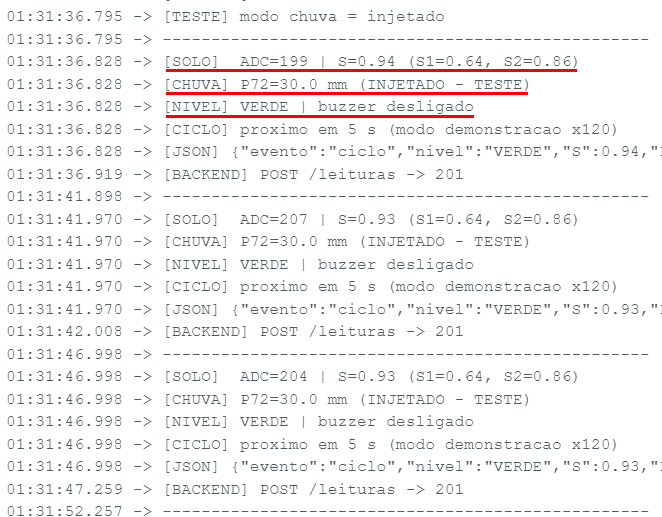
\includegraphics[width=\textwidth]{figures/cap5/F04_serial.png}}
\caption{Caso F04: monitor serial com $S$ de 0,93 a 0,94 e $P_{72} = 30$\,mm, nível VERDE}
\label{fig:res-f04-serial}
\fonte{Autora, 2026.}
\end{figure}

O painel recebeu a leitura do protótipo físico sem dados de energia e
exibiu ``Esta leitura não traz dados de energia''
(\autoref{fig:res-painel-f04}).

\begin{figure}[H]
\centering
\fbox{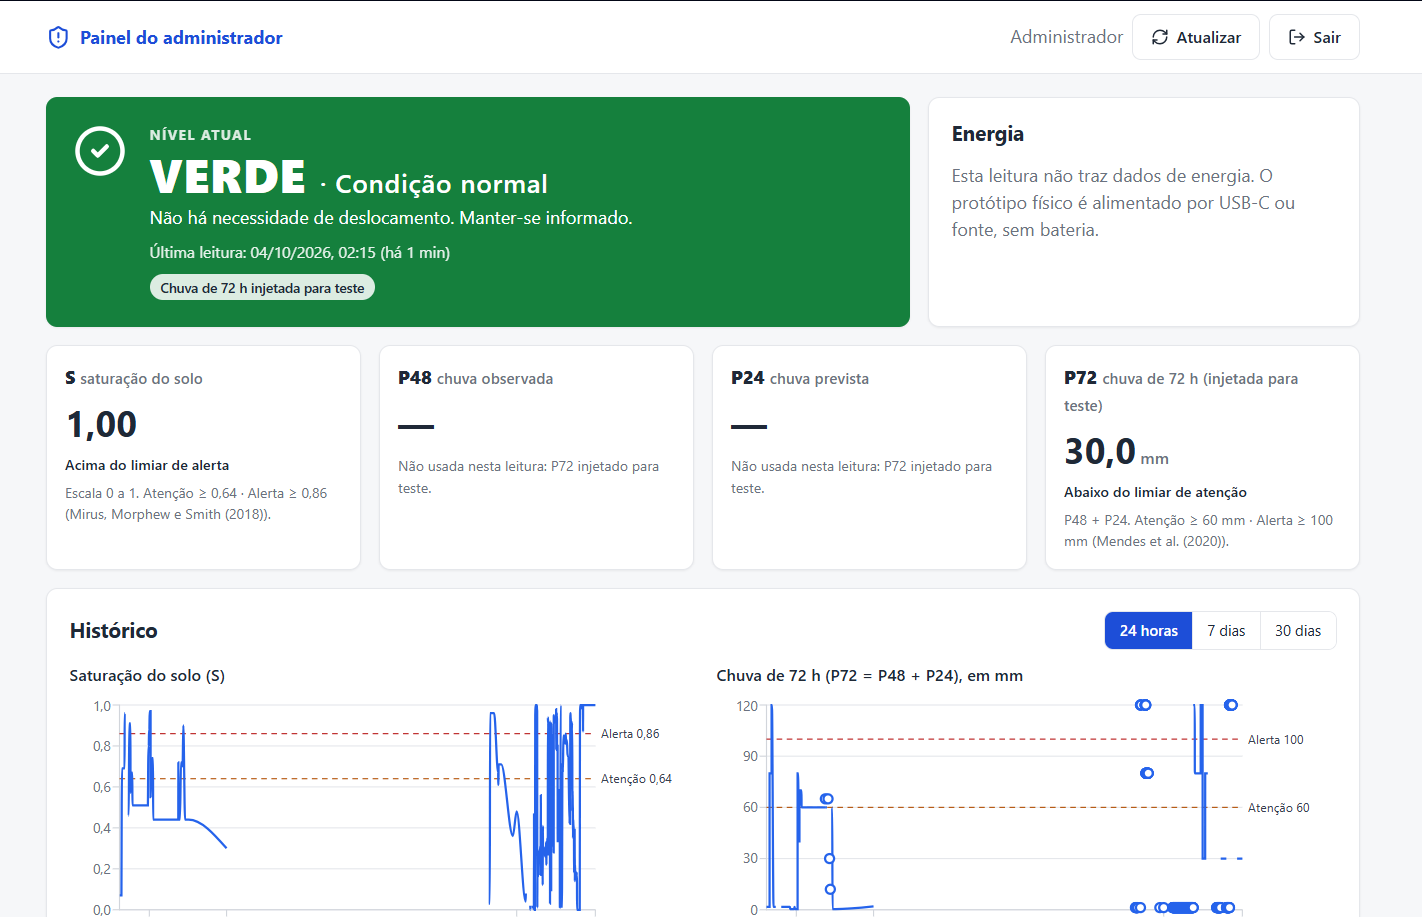
\includegraphics[width=\textwidth]{figures/cap5/P_painel_fisico_verde.png}}
\caption{Painel com leitura do protótipo físico no cenário do caso F04: VERDE, $S = 1{,}00$ e $P_{72} = 30$\,mm informado}
\label{fig:res-painel-f04}
\fonte{Autora, 2026.}
\end{figure}

\paragraph*{Caso F05 --- sonda desconectada}

Entrada: sonda desconectada do módulo e $P_{72} = 80$\,mm. Saída
esperada: AMARELO, definido só pela chuva. Saída observada: leitura
1023, ``\texttt{HIGROMETRO INDISPONIVEL}'', nível AMARELO e LED amarelo
aceso (\autoref{fig:res-f05-foto} e \autoref{fig:res-f05-serial}).

\begin{figure}[H]
\centering
\fbox{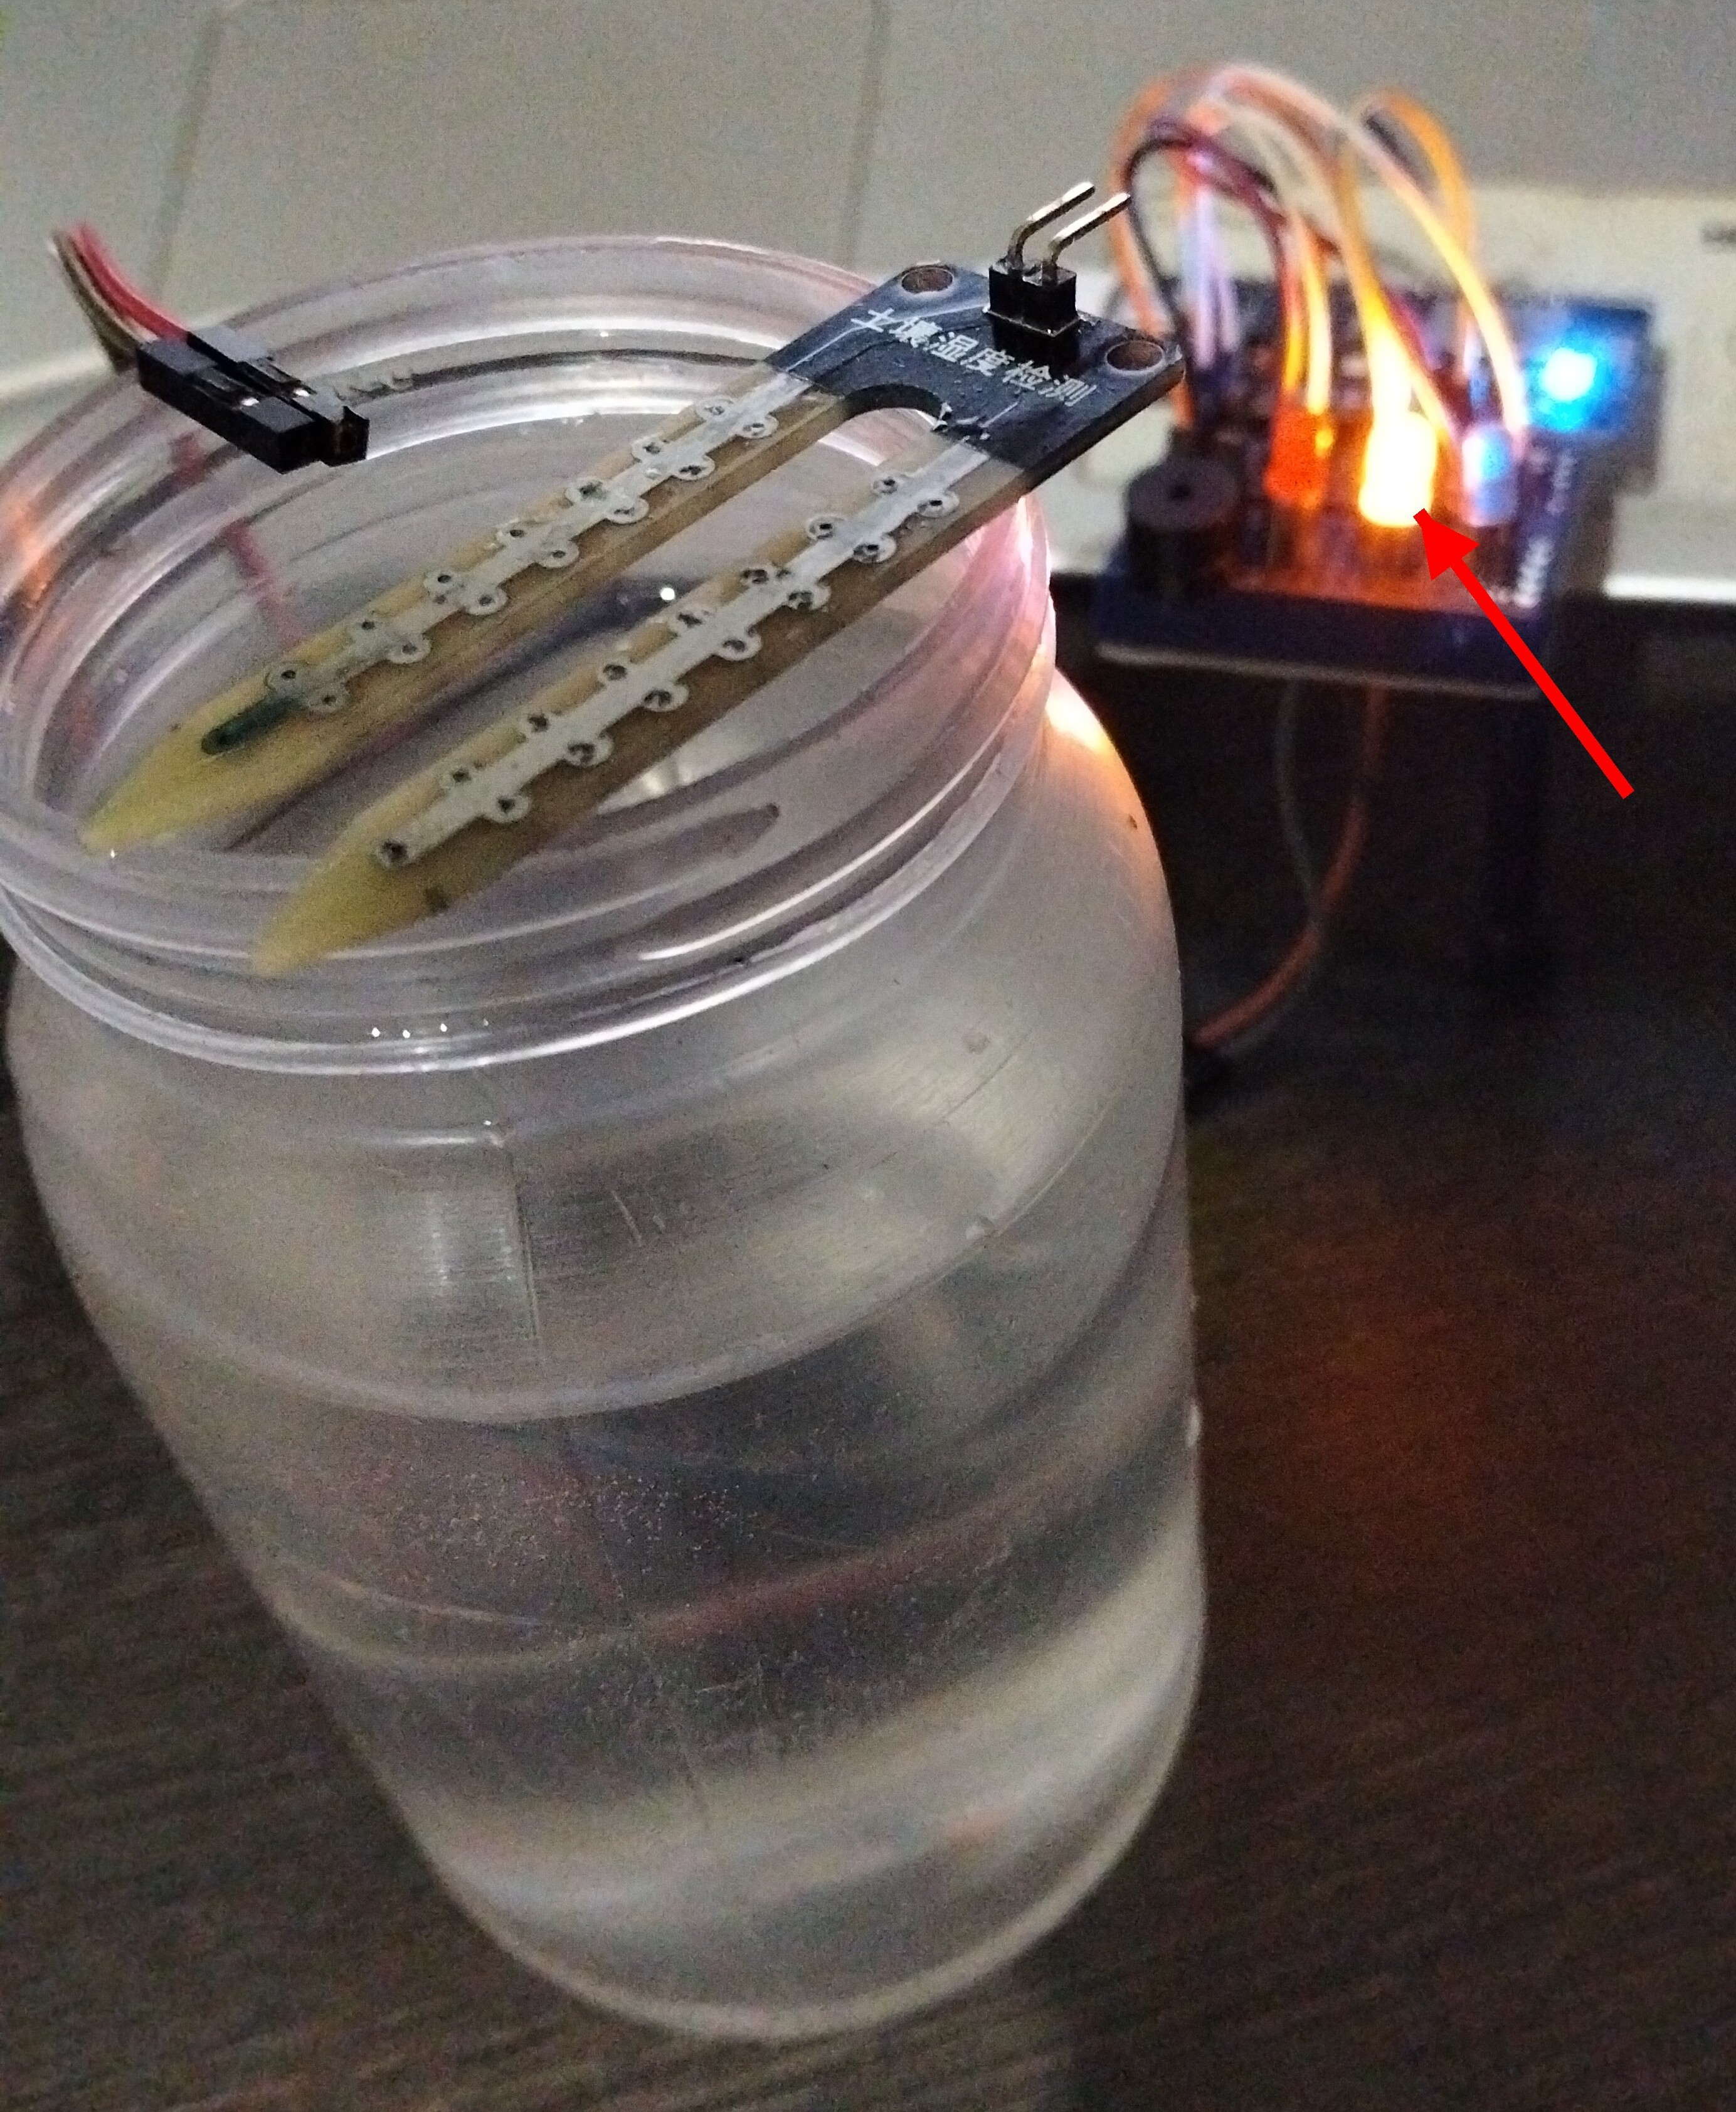
\includegraphics[height=0.42\textheight,keepaspectratio]{figures/cap5/F05_foto.jpg}}
\caption{Caso F05 no protótipo físico: sonda desconectada e LED amarelo aceso}
\label{fig:res-f05-foto}
\fonte{Autora, 2026.}
\end{figure}

\begin{figure}[H]
\centering
\fbox{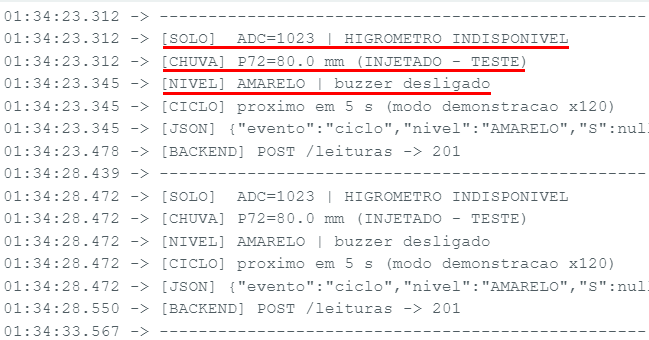
\includegraphics[width=\textwidth]{figures/cap5/F05_serial.png}}
\caption{Caso F05: monitor serial com higrômetro indisponível e nível AMARELO pela chuva}
\label{fig:res-f05-serial}
\fonte{Autora, 2026.}
\end{figure}

\paragraph*{Caso F06 --- sonda imersa sem dados de chuva}

Entrada: sonda imersa ($S = 1{,}00$) e APIs indisponíveis
(\texttt{chuva na}). Saída esperada: AMARELO, pelo caso especial. Saída
observada: ``\texttt{SEM DADOS DE CHUVA}'', ``\texttt{AMARELO | buzzer
desligado}'' e LED amarelo aceso (\autoref{fig:res-f06-foto} e
\autoref{fig:res-f06-serial}).

\begin{figure}[H]
\centering
\fbox{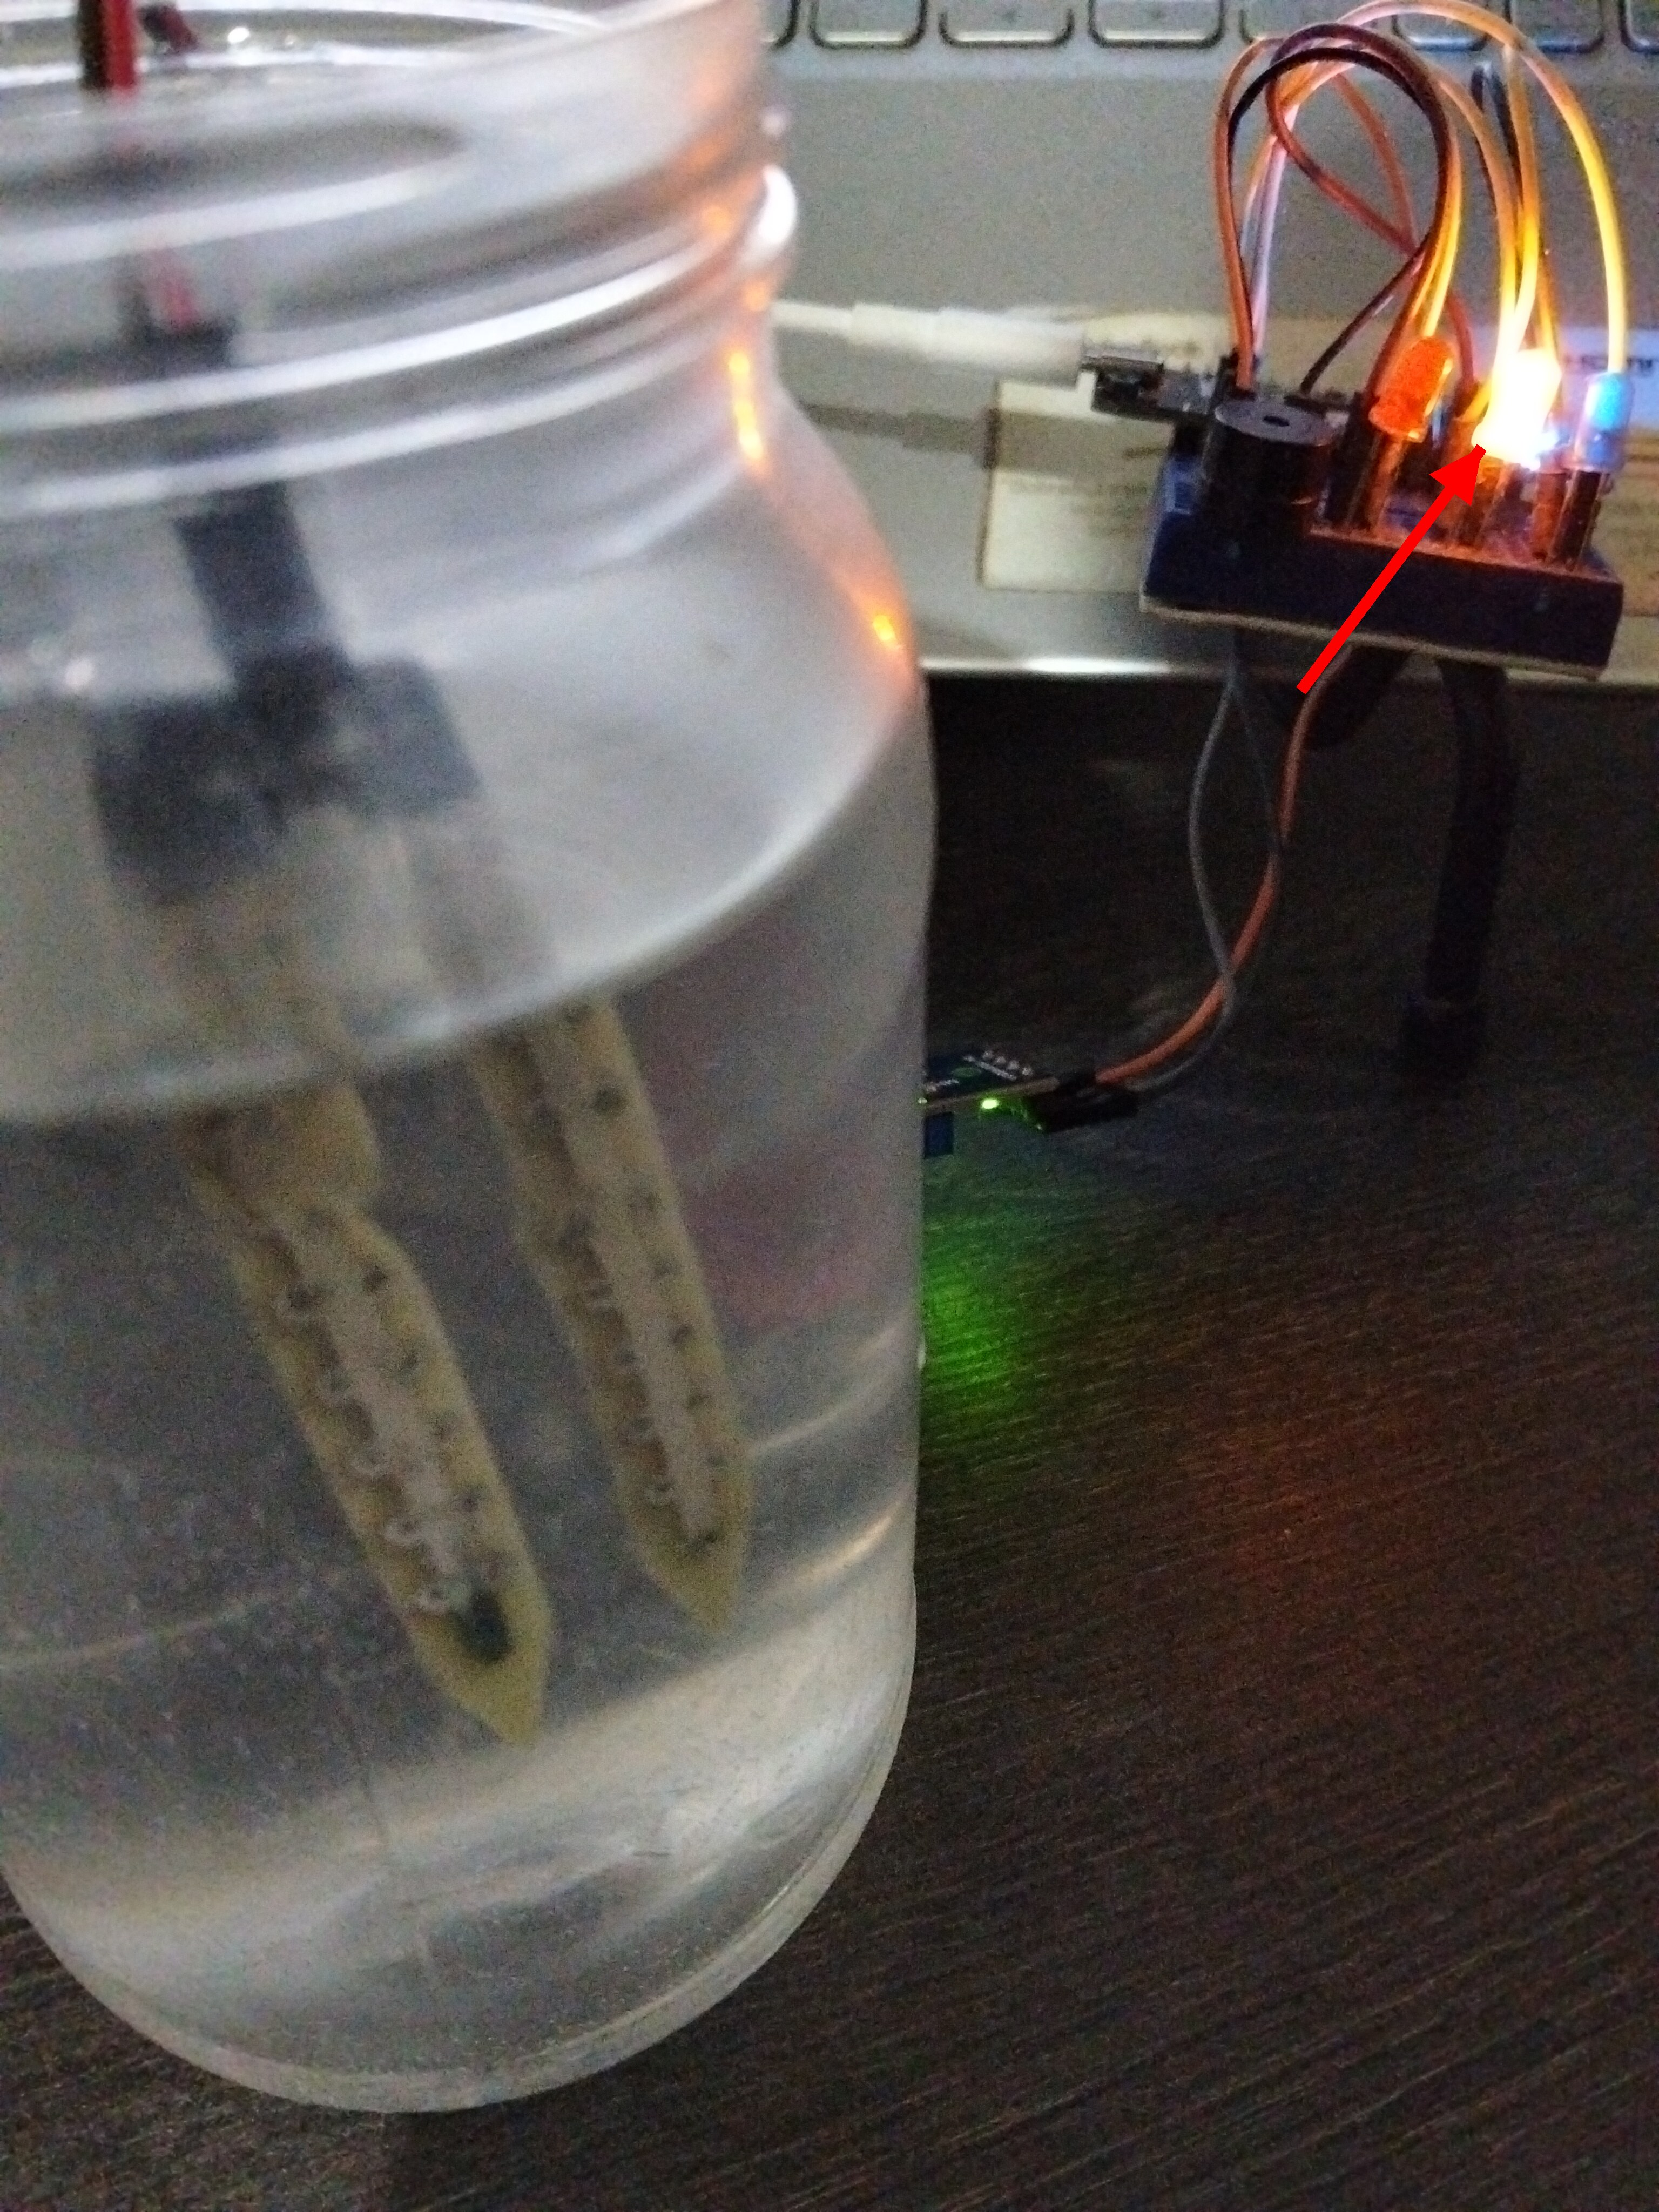
\includegraphics[height=0.42\textheight,keepaspectratio]{figures/cap5/F06_foto.jpg}}
\caption{Caso F06 no protótipo físico: sonda imersa, sem dados de chuva e LED amarelo aceso}
\label{fig:res-f06-foto}
\fonte{Autora, 2026.}
\end{figure}

\begin{figure}[H]
\centering
\fbox{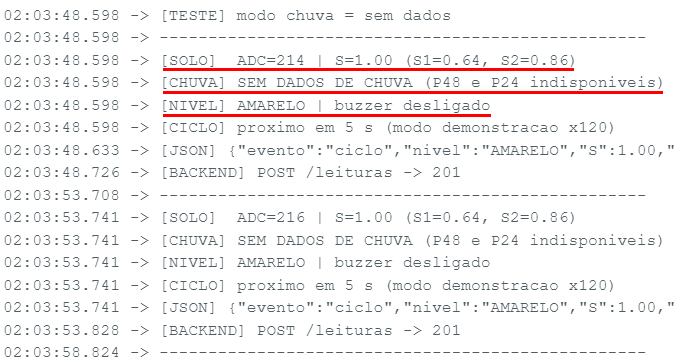
\includegraphics[width=\textwidth]{figures/cap5/F06_serial.png}}
\caption{Caso F06: monitor serial com $S = 1{,}00$, sem dados de chuva, nível AMARELO (caso especial)}
\label{fig:res-f06-serial}
\fonte{Autora, 2026.}
\end{figure}

\paragraph*{Caso F07 --- APIs reais}

Entrada: consulta às APIs em 4 de outubro de 2026. A BNDMET retornou
0,0\,mm para 2 de outubro e nenhum valor para 3 de outubro, e a
previsão foi de 1,3\,mm. Saída esperada: dados incompletos, com mínimo
de 1,3\,mm tratado como falta de dados de chuva.

Saída observada: ``\texttt{DADOS DE CHUVA INCOMPLETOS - P72 >= 1.3
mm}'' e ``\texttt{Minimo abaixo de P1}''. O nível foi VERDE com
$S = 0{,}00$ e $S = 0{,}83$, e AMARELO com $S = 1{,}00$, pelo caso
especial (\autoref{fig:res-f07}).

O painel exibiu o nível AMARELO, o aviso de um dia sem registro na
estação e o cartão ``Dados de chuva incompletos --- P72 $\geq$ 1,3 mm''
(\autoref{fig:res-painel-f07}).

\begin{figure}[H]
\centering
\fbox{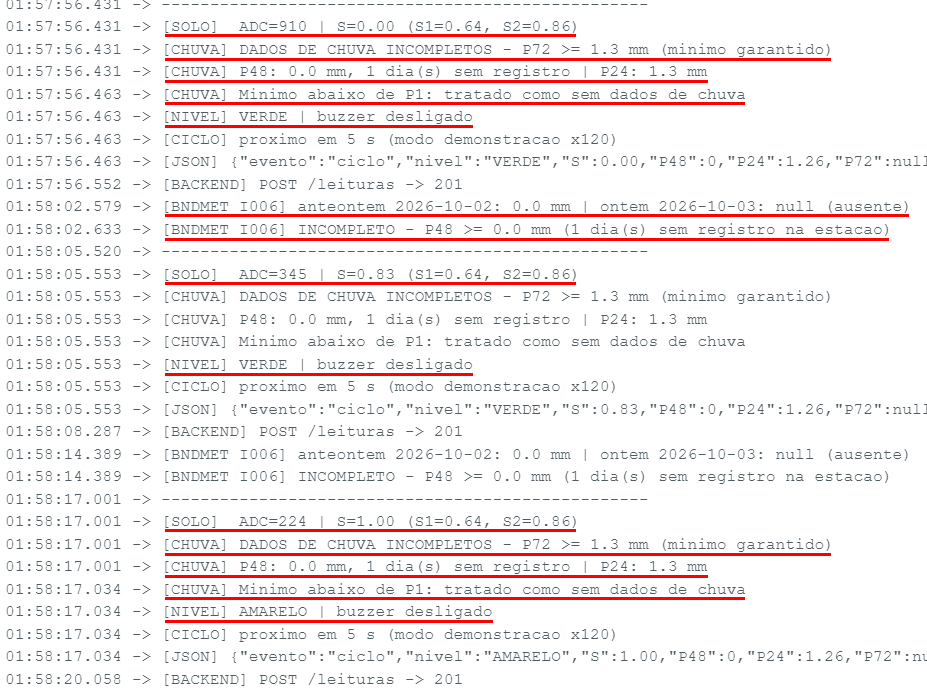
\includegraphics[width=\textwidth]{figures/cap5/F07_apis_reais.png}}
\caption{Caso F07: APIs reais com um dia sem registro na BNDMET, mínimo de 1,3\,mm}
\label{fig:res-f07}
\fonte{Autora, 2026.}
\end{figure}

\begin{figure}[H]
\centering
\fbox{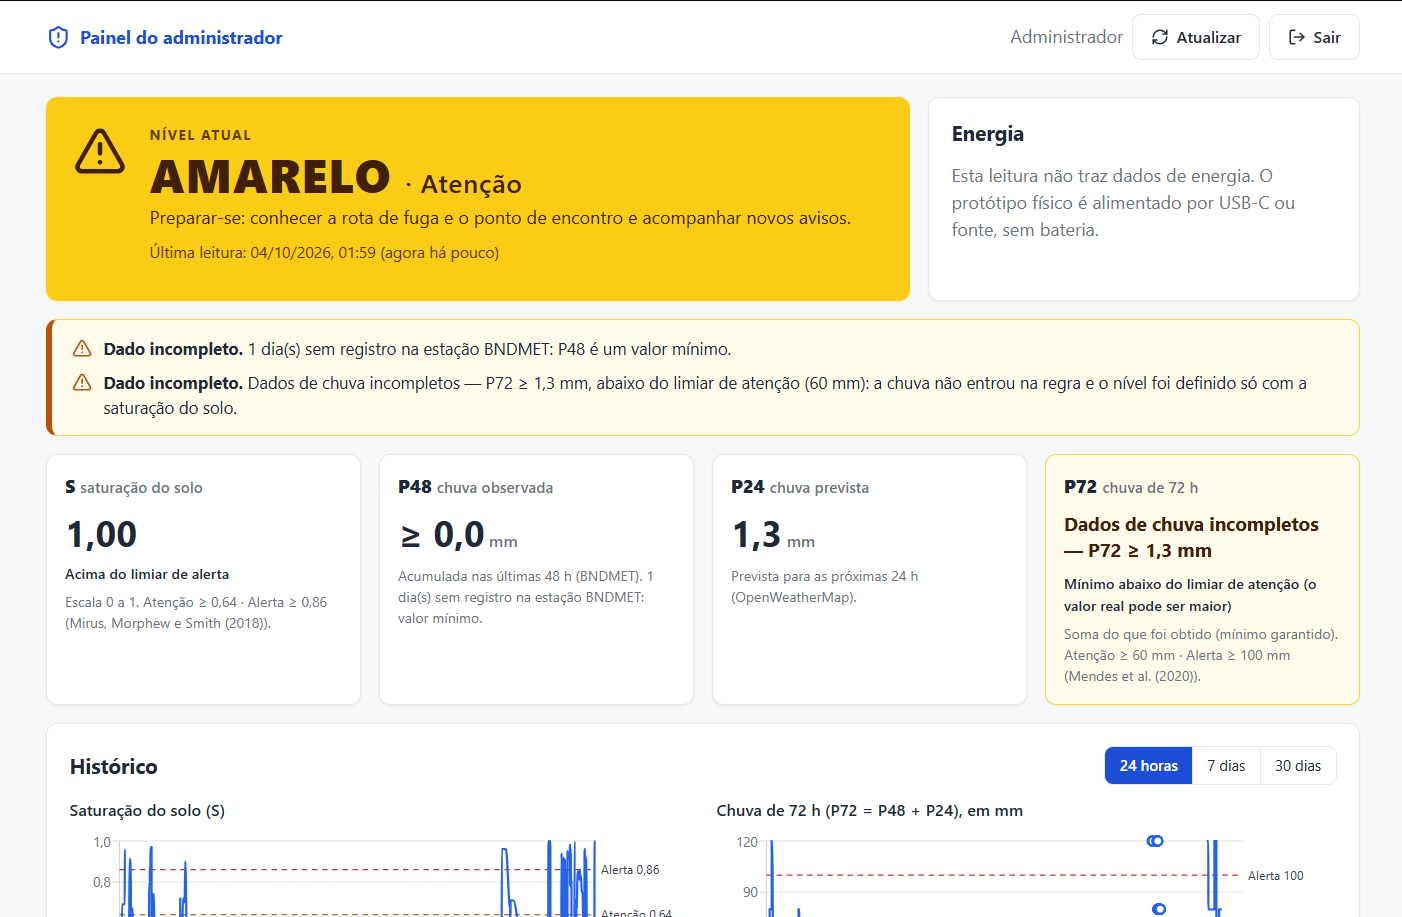
\includegraphics[width=\textwidth]{figures/cap5/P_painel_fisico_amarelo.png}}
\caption{Painel com leitura do protótipo físico no caso F07: AMARELO com $S = 1{,}00$ e dados de chuva incompletos}
\label{fig:res-painel-f07}
\fonte{Autora, 2026.}
\end{figure}

\paragraph*{Caso F08 --- dados incompletos com mínimo acima de $P_2$}

Entrada: sonda imersa ($S = 1{,}00$) e \texttt{chuva parcial 120}.
Saída esperada: VERMELHO, avaliado com o mínimo garantido, com o
\textit{buzzer} acionado. Saída observada: ``\texttt{DADOS DE CHUVA
INCOMPLETOS - P72 >= 120.0 mm}'', ``\texttt{VERMELHO | buzzer
LIGADO}'' e LED vermelho aceso (\autoref{fig:res-f08-foto} e
\autoref{fig:res-f08-serial}).

\begin{figure}[H]
\centering
\fbox{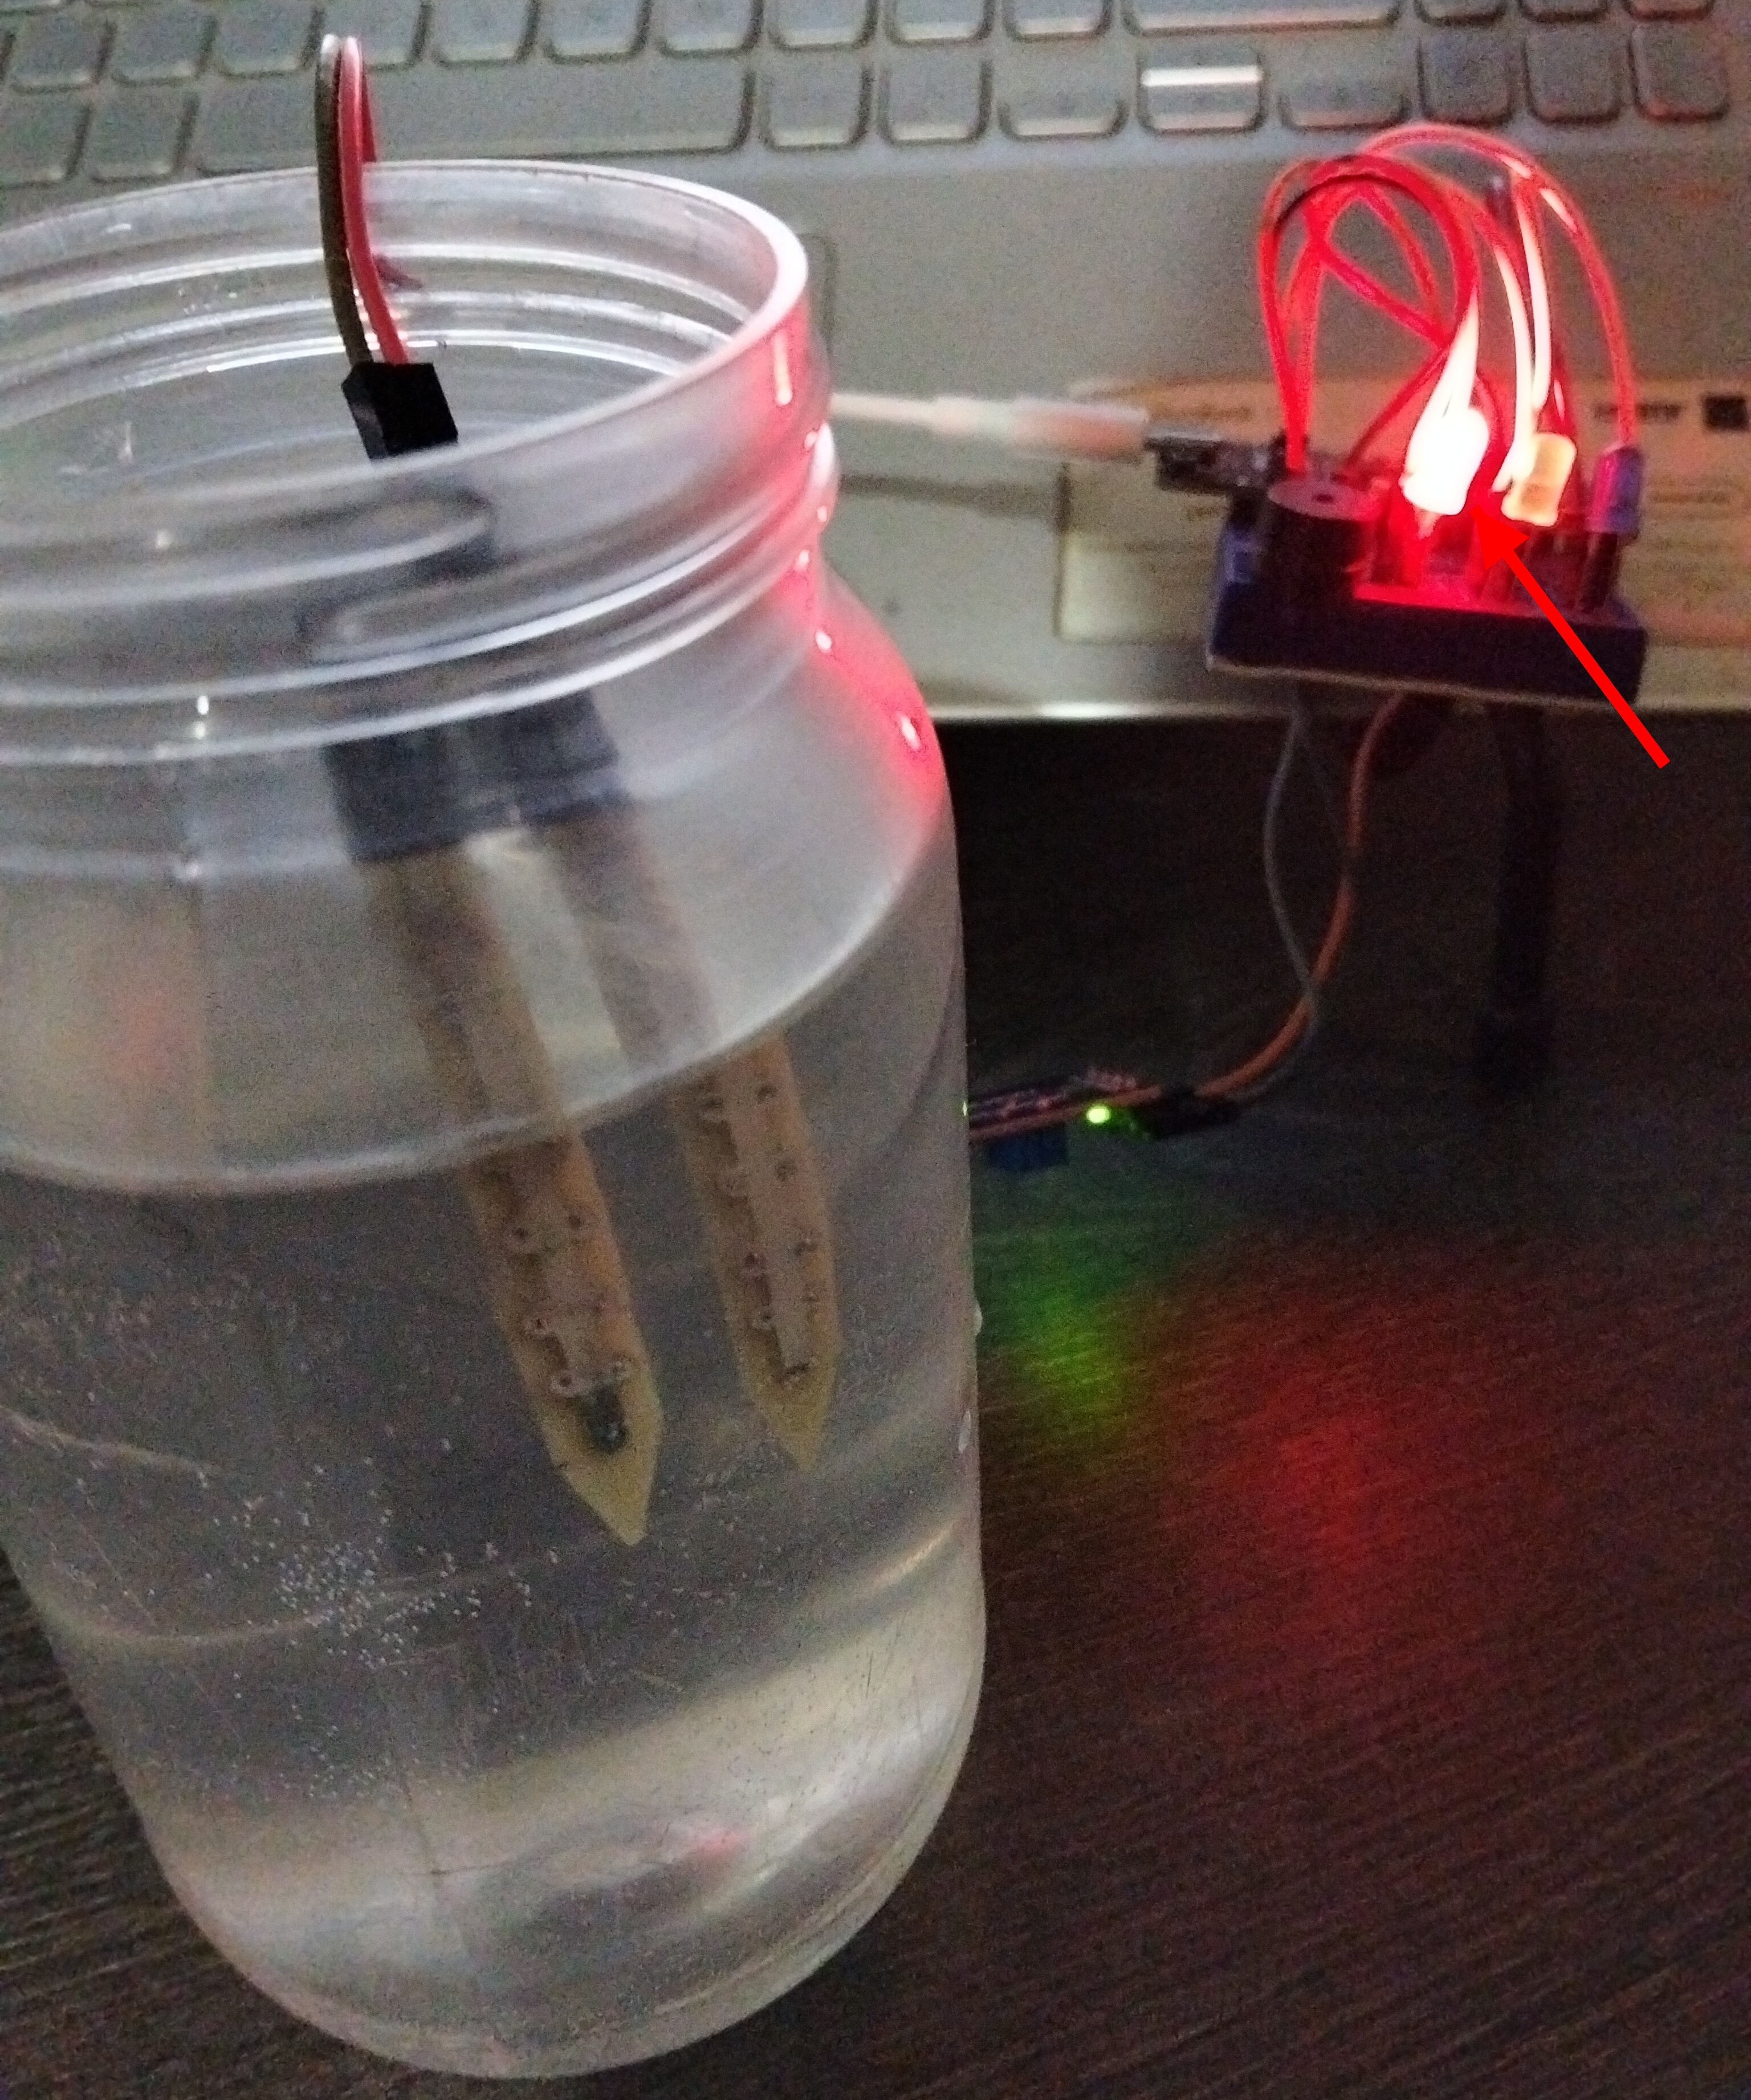
\includegraphics[height=0.42\textheight,keepaspectratio]{figures/cap5/F08_foto.jpg}}
\caption{Caso F08 no protótipo físico: sonda imersa, dados de chuva incompletos e LED vermelho aceso}
\label{fig:res-f08-foto}
\fonte{Autora, 2026.}
\end{figure}

\begin{figure}[H]
\centering
\fbox{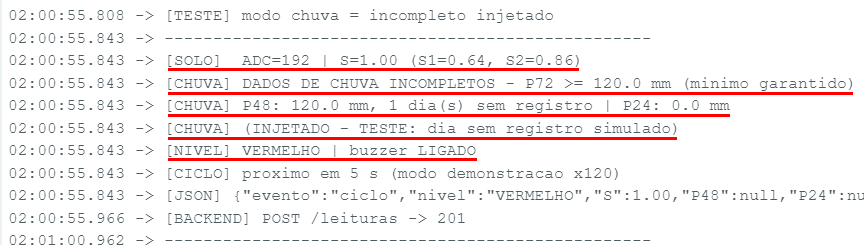
\includegraphics[width=\textwidth]{figures/cap5/F08_serial.png}}
\caption{Caso F08: monitor serial com mínimo garantido de 120\,mm, nível VERMELHO e \textit{buzzer} ligado}
\label{fig:res-f08-serial}
\fonte{Autora, 2026.}
\end{figure}

Em uma leitura anterior do protótipo físico, com dados de chuva
completos ($P_{48} = 2{,}0$\,mm e $P_{24} = 0{,}0$\,mm) e $S = 0{,}30$,
o painel exibiu o nível VERDE (\autoref{fig:res-w14}).

\begin{figure}[H]
\centering
\fbox{\includegraphics[width=\textwidth,trim=232 1070 236 0,clip]{figures/cap5/W14_painel_fisico.pdf}}
\caption{Painel com leitura do protótipo físico e dados de chuva completos: VERDE, sem dados de energia}
\label{fig:res-w14}
\fonte{Autora, 2026.}
\end{figure}

% =============================================================
\section{Plataforma \textit{Web}}
\label{sec:res-web}
% =============================================================

A plataforma foi testada nas três telas descritas na
\autoref{subsec:arquitetura}: a página inicial, o acesso do
administrador e o painel. Os estados do painel ligados aos casos de
teste foram apresentados nas \autoref{sec:res-simulacao} a
\autoref{sec:res-fisico}.

% -------------------------------------------------------------
\subsection{Página Inicial e Cadastro do Morador}
\label{subsec:res-landing}
% -------------------------------------------------------------

Entrada: acesso à página inicial. Saída esperada: resumo do sistema e
botão de cadastro. Saída observada: a página apresentou o que o sistema
acompanha (saturação do solo, chuva das últimas 48~h e previsão para
24~h) e o botão ``Quero receber alertas'' (\autoref{fig:res-w01}).

\begin{figure}[H]
\centering
\fbox{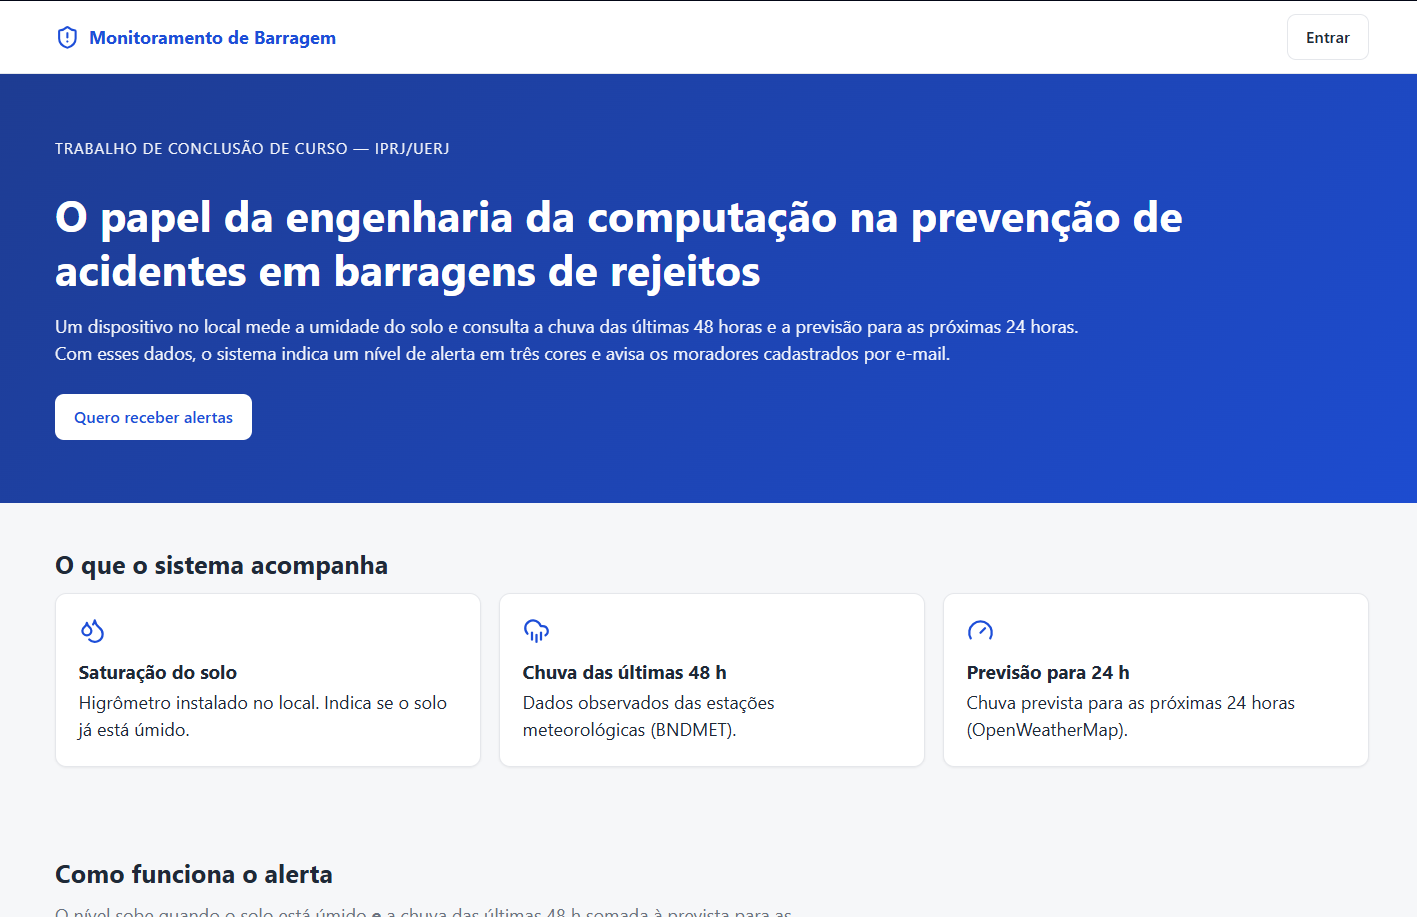
\includegraphics[width=\textwidth]{figures/cap5/W01_landing.png}}
\caption{Página inicial da plataforma \textit{web}}
\label{fig:res-w01}
\fonte{Autora, 2026.}
\end{figure}

Entrada: formulário preenchido com nome, e-mail, telefone e localidade
(\autoref{fig:res-w02a}). Saída esperada: cadastro do morador. Saída
observada: mensagem ``Cadastro feito'', com o e-mail que receberá os
avisos (\autoref{fig:res-w02b}).

\begin{figure}[H]
\centering
\fbox{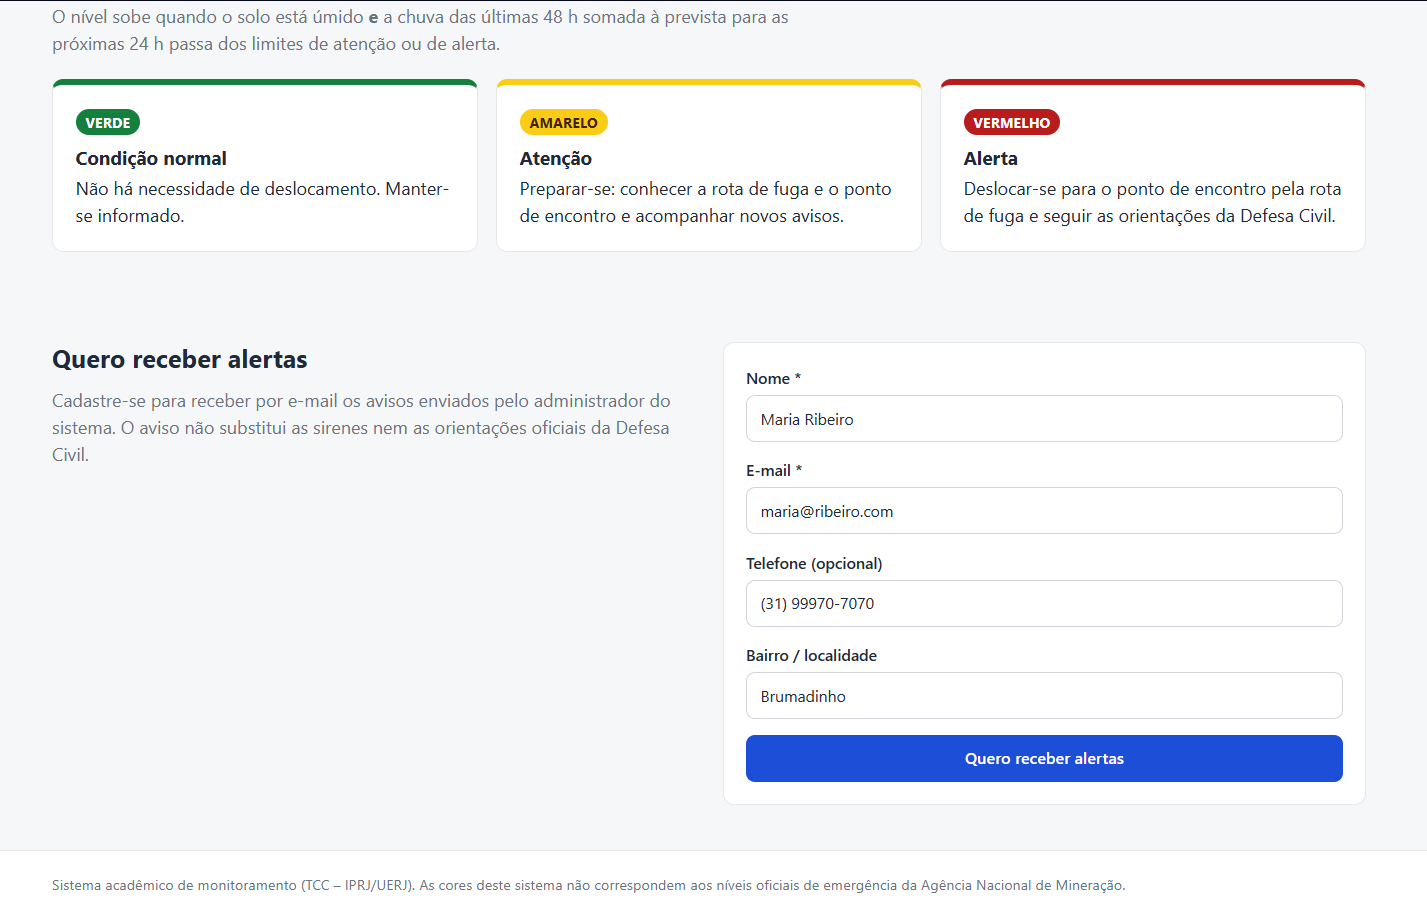
\includegraphics[width=\textwidth]{figures/cap5/W02_cadastro_preenchido.png}}
\caption{Explicação dos três níveis e formulário de cadastro preenchido (dados fictícios)}
\label{fig:res-w02a}
\fonte{Autora, 2026.}
\end{figure}

\begin{figure}[H]
\centering
\fbox{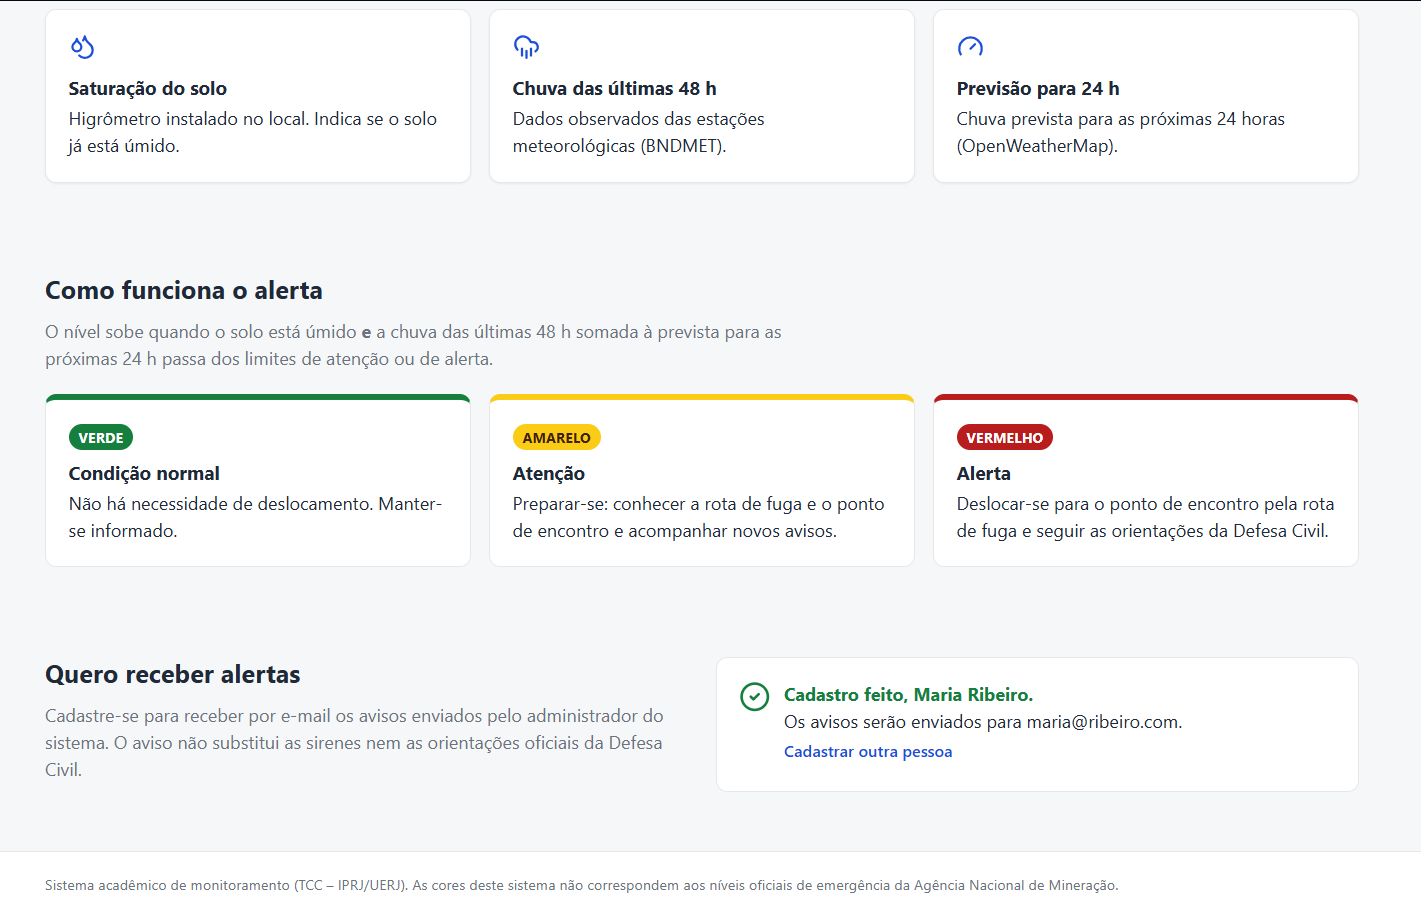
\includegraphics[width=\textwidth]{figures/cap5/W02_cadastro_ok.png}}
\caption{Confirmação do cadastro do morador}
\label{fig:res-w02b}
\fonte{Autora, 2026.}
\end{figure}

% -------------------------------------------------------------
\subsection{Acesso do Administrador e Painel}
\label{subsec:res-painel}
% -------------------------------------------------------------

Entrada: e-mail e senha do administrador (\autoref{fig:res-w03}). Saída
esperada: acesso ao painel. Saída observada: o painel foi aberto. Sem
nenhuma leitura no banco de dados, ele exibiu ``Nenhuma leitura recebida
do dispositivo'' e os indicadores como indisponíveis
(\autoref{fig:res-w04}).

\begin{figure}[H]
\centering
\fbox{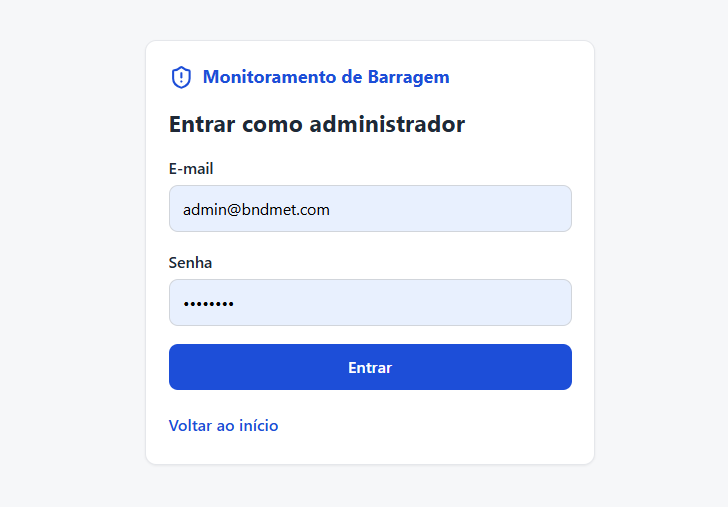
\includegraphics[width=0.75\textwidth]{figures/cap5/W03_login.png}}
\caption{Tela de acesso do administrador}
\label{fig:res-w03}
\fonte{Autora, 2026.}
\end{figure}

\begin{figure}[H]
\centering
\fbox{\includegraphics[width=\textwidth,height=0.7\textheight,keepaspectratio,trim=232 0 236 0,clip]{figures/cap5/W04_painel_sem_leitura.pdf}}
\caption{Painel do administrador antes da primeira leitura}
\label{fig:res-w04}
\fonte{Autora, 2026.}
\end{figure}

Após os casos de teste, o histórico exibiu os gráficos de $S$ e de
$P_{72}$, com as linhas dos limiares e o nível de cada leitura
(\autoref{fig:res-w15}). Em tela de celular, o painel foi exibido em
uma coluna, sem rolagem lateral (\autoref{fig:res-w20}).

\begin{figure}[H]
\centering
\fbox{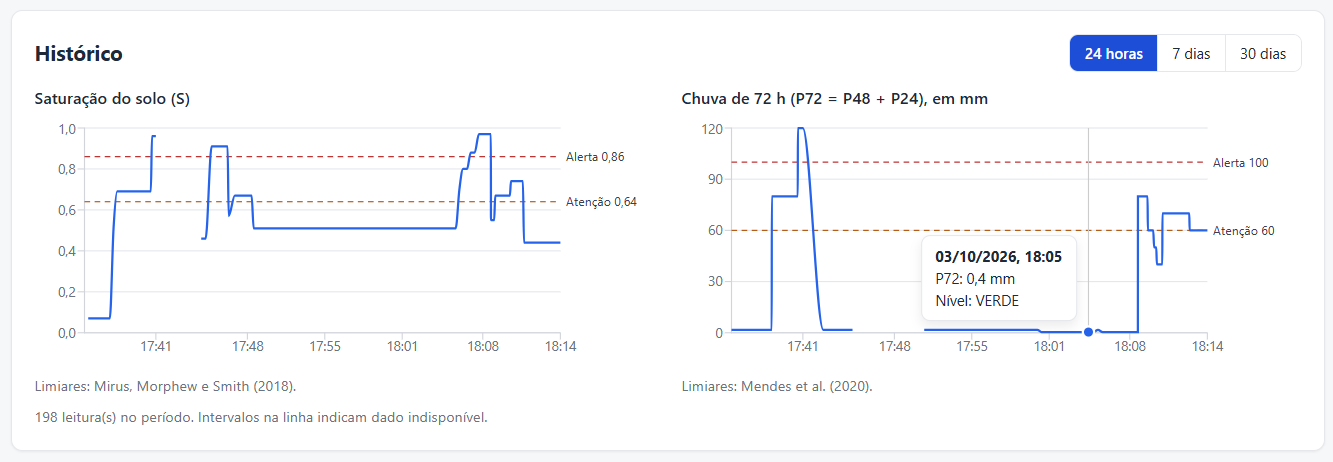
\includegraphics[width=\textwidth]{figures/cap5/W15_historico.png}}
\caption{Histórico de $S$ e de $P_{72}$ após os casos de teste (valores da simulação)}
\label{fig:res-w15}
\fonte{Autora, 2026.}
\end{figure}

\begin{figure}[H]
\centering
\fbox{\includegraphics[height=0.8\textheight,trim=0 1700 0 0,clip,keepaspectratio]{figures/cap5/W20_painel_celular.pdf}}
\caption{Painel do administrador em tela de celular (parte superior)}
\label{fig:res-w20}
\fonte{Autora, 2026.}
\end{figure}

% -------------------------------------------------------------
\subsection{Envio do E-mail de Alerta}
\label{subsec:res-envio}
% -------------------------------------------------------------

O envio foi testado logo após o caso C09, com o nível atual VERMELHO e
cinco moradores cadastrados. Entrada: escolha do nível VERMELHO no
painel. Saída esperada: mensagem-modelo do nível
(\autoref{qua:mensagens-alerta}), com os dados da última leitura, e
pedido de confirmação.

Saída observada: o assunto e a mensagem do nível VERMELHO foram
preenchidos com a leitura de 4 de outubro de 2026, às 12h25
($S = 0{,}94$ e $P_{72} = 120{,}0$\,mm), e o painel pediu a confirmação
do envio para cinco moradores (\autoref{fig:res-w16}).

\begin{figure}[H]
\centering
\fbox{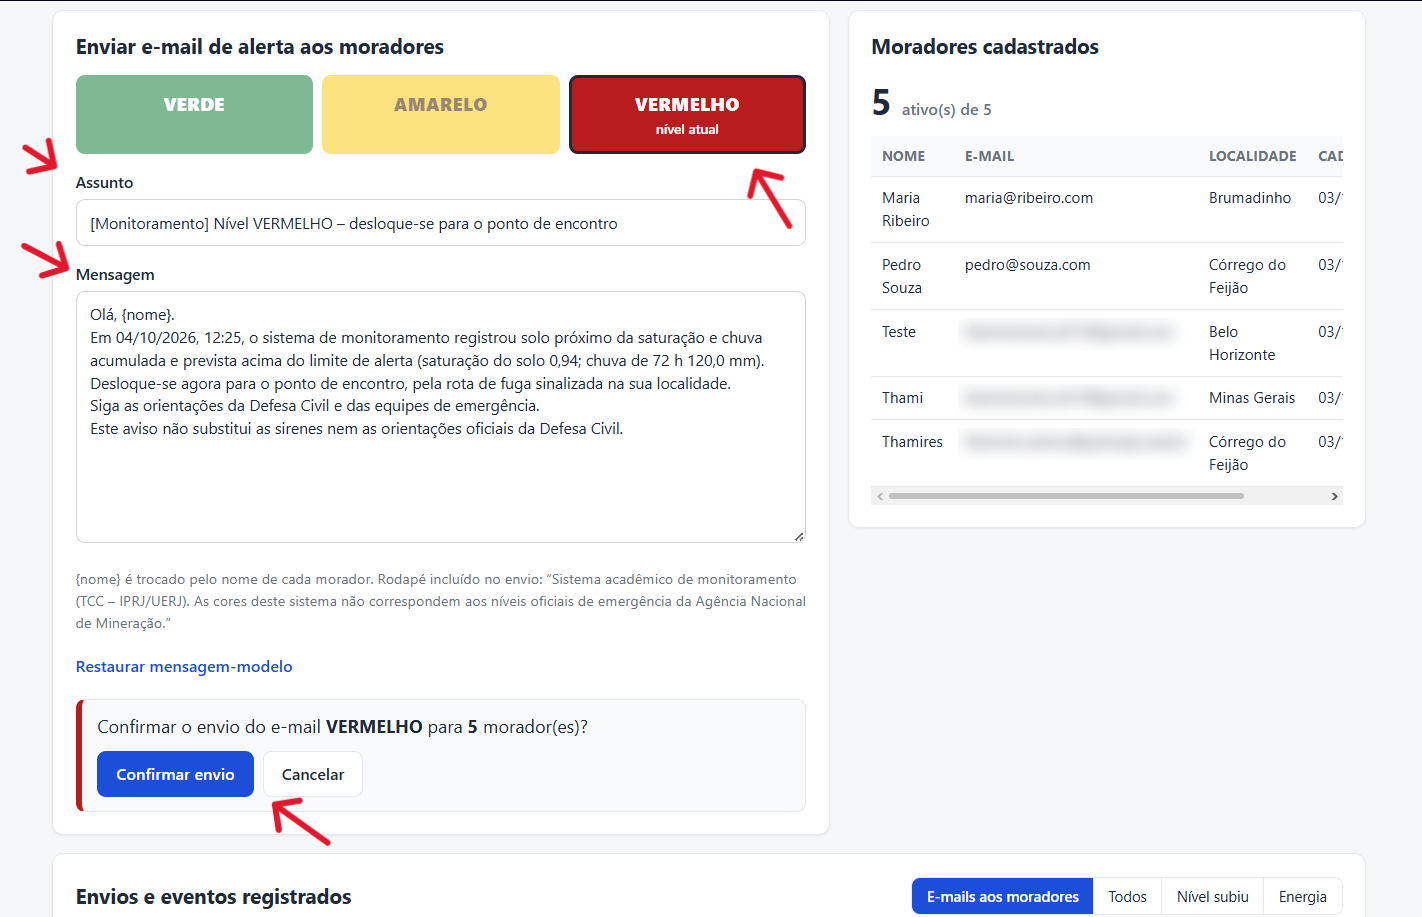
\includegraphics[width=\textwidth]{figures/cap5/W16_envio_confirmacao.png}}
\caption{Envio do e-mail de alerta: nível VERMELHO escolhido e pedido de confirmação (e-mails dos moradores ocultados)}
\label{fig:res-w16}
\fonte{Autora, 2026.}
\end{figure}

Após a confirmação, o botão passou a ``Enviando...''
(\autoref{fig:res-w17a}). Ao final, o painel informou ``Enviado a 5 de
5 morador(es)'', e o envio foi registrado com data, nível,
administrador e número de e-mails (\autoref{fig:res-w17b}).

\begin{figure}[H]
\centering
\fbox{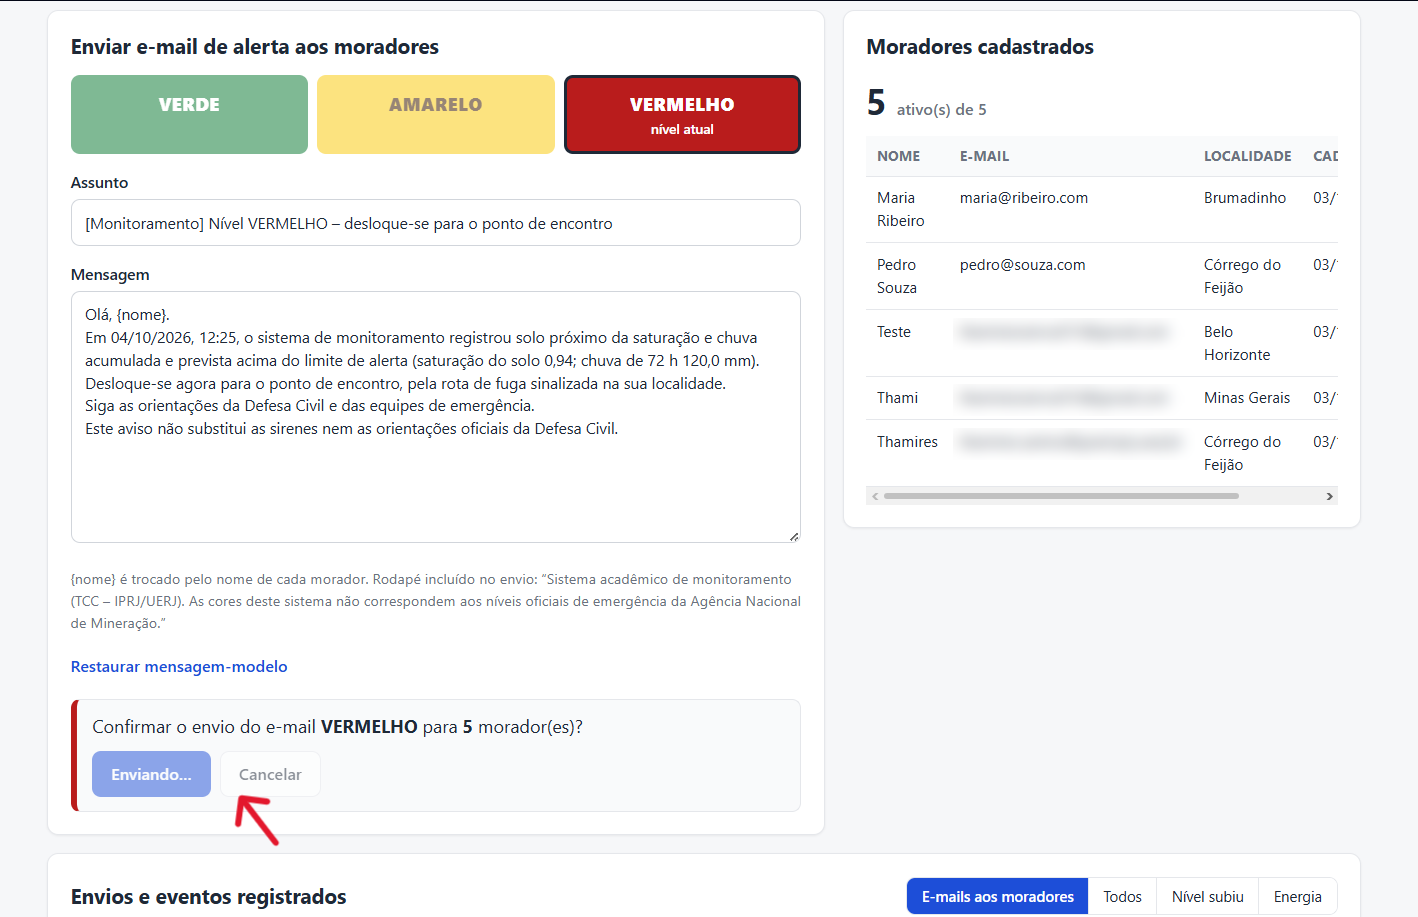
\includegraphics[width=\textwidth]{figures/cap5/W17_envio_registrado_durante.png}}
\caption{Envio do e-mail de alerta em andamento (e-mails dos moradores ocultados)}
\label{fig:res-w17a}
\fonte{Autora, 2026.}
\end{figure}

\begin{figure}[H]
\centering
\fbox{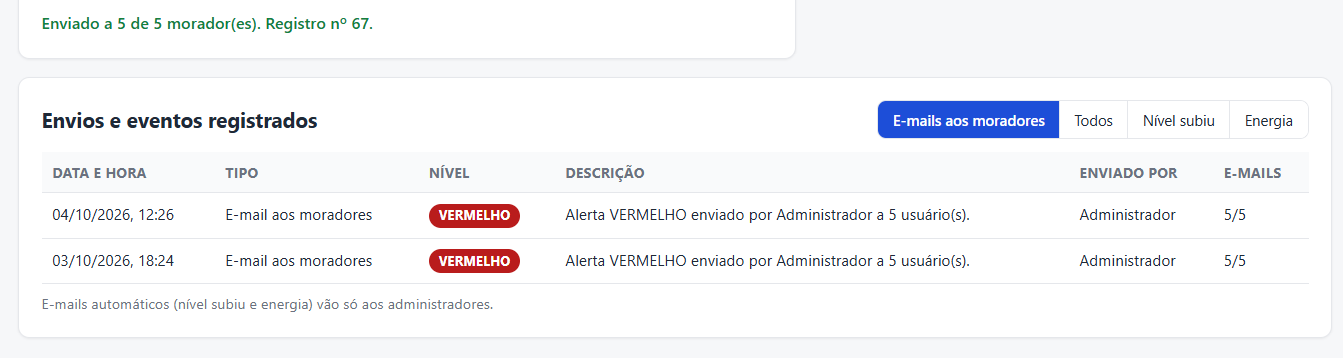
\includegraphics[width=\textwidth]{figures/cap5/W17_envio_registrado_depois.png}}
\caption{Resultado do envio e registro na lista de envios}
\label{fig:res-w17b}
\fonte{Autora, 2026.}
\end{figure}

O e-mail chegou à caixa de entrada do morador com o assunto do nível
VERMELHO, a mensagem e o rodapé que informa que as cores não
correspondem aos níveis oficiais de emergência
(\autoref{fig:res-w19}). A mensagem recebida trouxe os valores da
leitura usada no envio ($S = 0{,}94$ e $P_{72} = 120{,}0$\,mm).

\begin{figure}[H]
\centering
\fbox{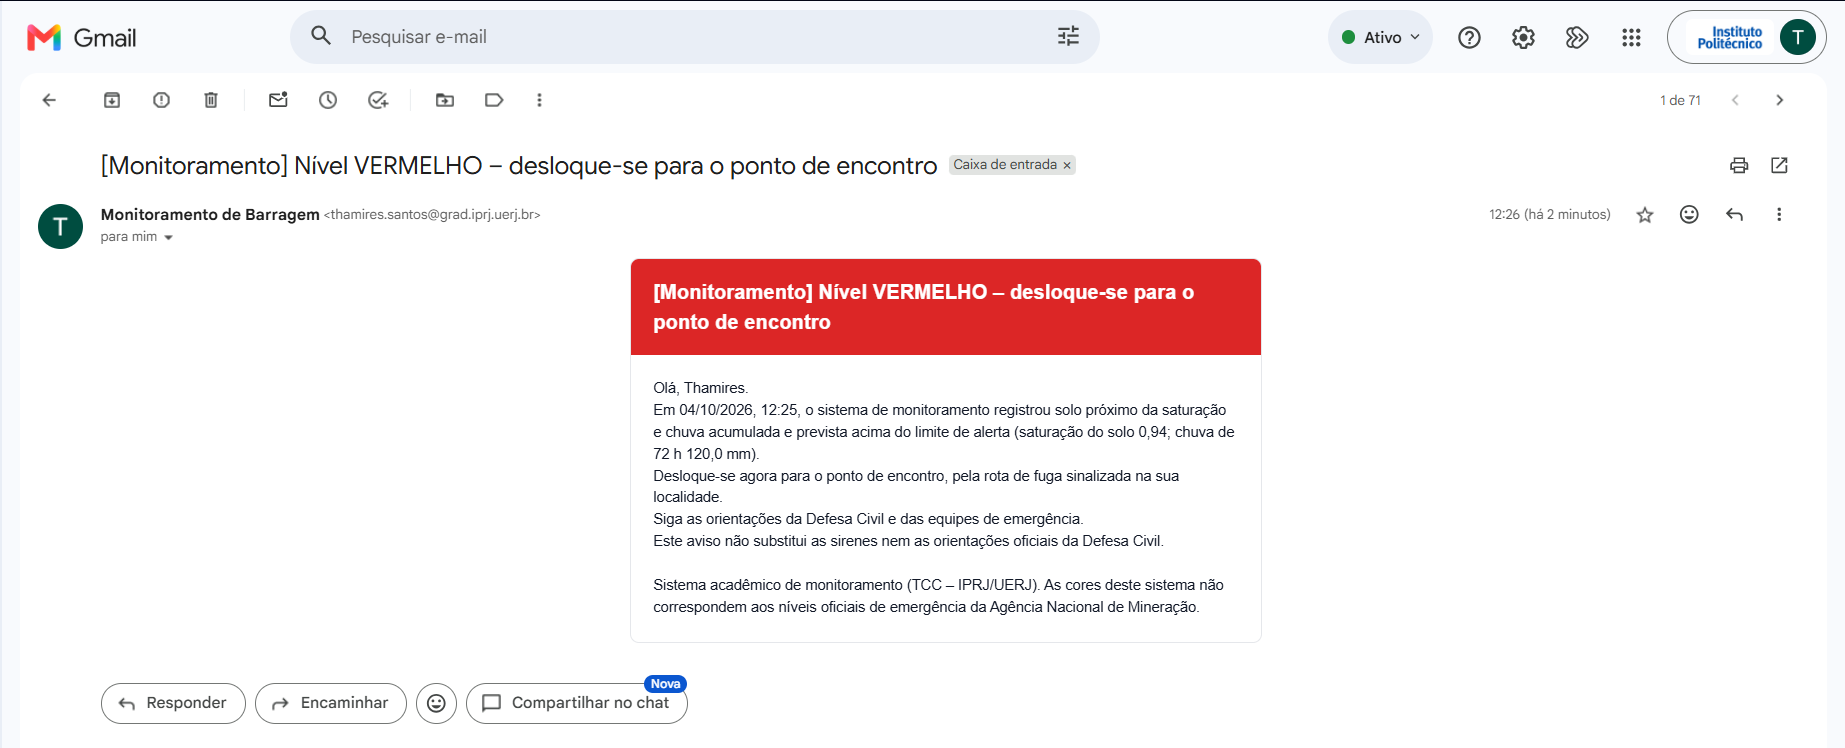
\includegraphics[width=\textwidth]{figures/cap5/W19_email_recebido.png}}
\caption{E-mail de alerta de nível VERMELHO recebido pelo morador}
\label{fig:res-w19}
\fonte{Autora, 2026.}
\end{figure}

Com o filtro ``Todos'', a lista exibiu o envio aos moradores e os
eventos automáticos: subidas de nível e mudanças de energia, como falta
de rede, bateria baixa, bateria crítica e falha de bateria. Cada evento
automático gerou um e-mail aos administradores (\autoref{fig:res-w18}).

\begin{figure}[H]
\centering
\fbox{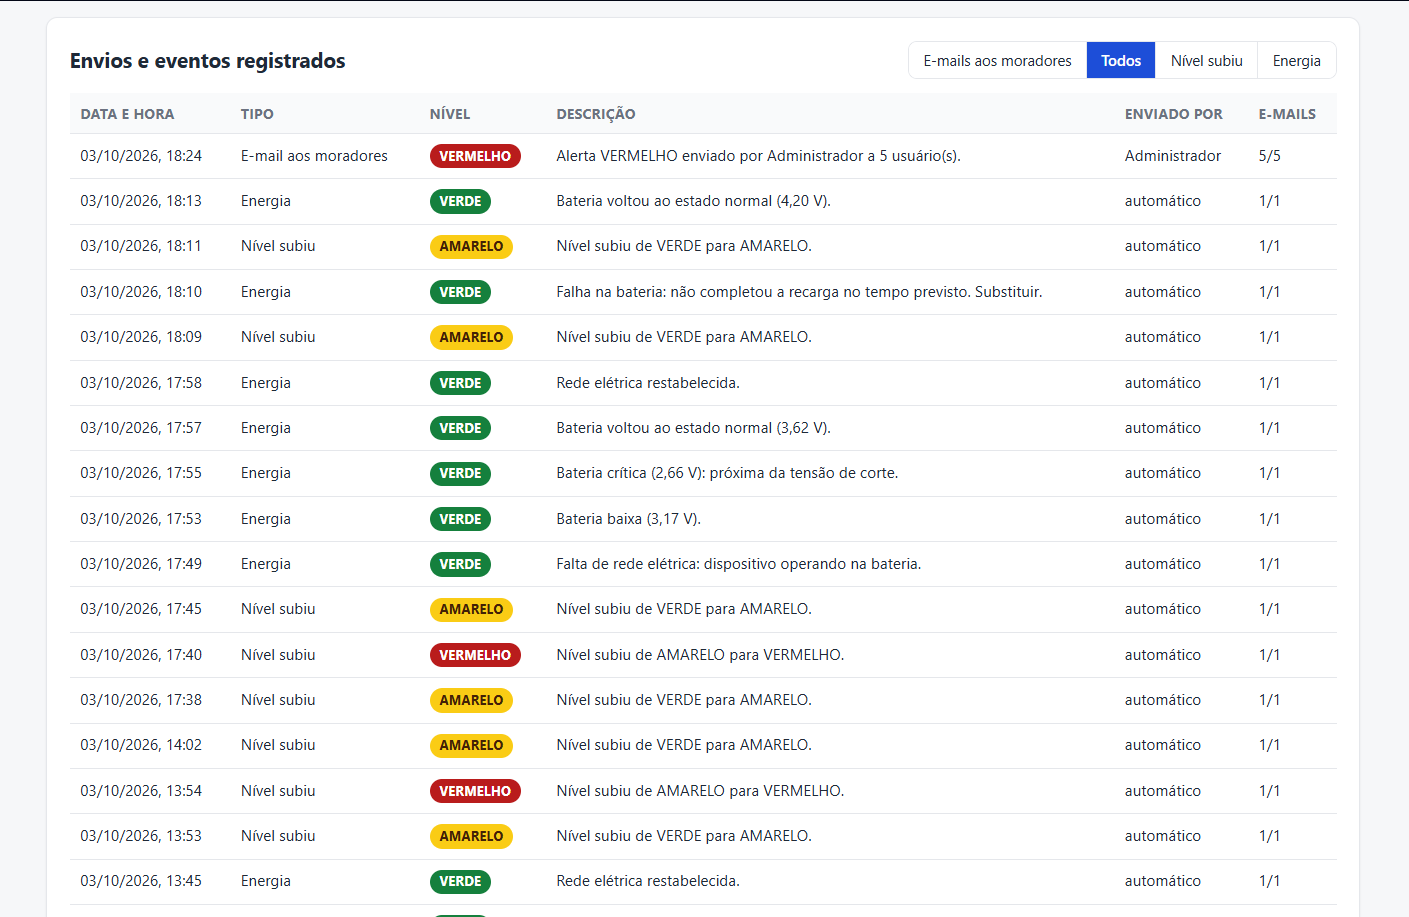
\includegraphics[width=\textwidth]{figures/cap5/W18_eventos_todos.png}}
\caption{Envios e eventos registrados, com o filtro ``Todos''}
\label{fig:res-w18}
\fonte{Autora, 2026.}
\end{figure}

% =============================================================
\section{Síntese dos Resultados}
\label{sec:res-sintese}
% =============================================================

A \autoref{tab:res-sintese} reúne os casos executados. Em todos eles,
a saída observada foi igual à saída esperada.

\begin{table}[htb]
\centering
\caption{Síntese dos casos de teste}
\label{tab:res-sintese}
\small
\begin{tabular}{p{3.6cm}p{2.2cm}p{2.0cm}p{6.2cm}}
\hline
\textbf{Grupo} & \textbf{Casos} & \textbf{Conformes} & \textbf{Observação} \\
\hline
Modelo de alerta (simulação) & C00 a C09 & 10 de 10 & C01, C04 e C07 com $P_{72}$ das APIs, na mesma faixa \\
Contingência (simulação) & X01 a X09 & 9 de 9 & X05 com dados reais das APIs \\
Energia (simulação) & E01 a E04 & 4 de 4 & Lógica dos estados; autonomia apenas calculada (\autoref{tab:autonomia}) \\
Protótipo físico & F01 a F08 & 8 de 8 & F07 com dado real ausente na BNDMET \\
Plataforma \textit{web} & Cadastro, acesso, painel e envio & todas & Envio a 5 de 5 moradores; eventos registrados \\
\hline
\end{tabular}
\fonte{Autora, 2026.}
\end{table}

Os casos verificam a lógica de decisão do \textit{firmware}, a
supervisão de energia e o fluxo da plataforma. Eles não avaliam o
comportamento do maciço nem a duração real da bateria, que permanece
como valor calculado.